\chapter{Evaluation}
    \section{Beschreibung der verwendeten Daten}
        Als Datenbasis wurde Cityscapes verwendet. Es ist ein bekannter Datensatz im Bereich der Bildsegmentierung und der Computer Vision. Der Datensatz wurde speziell für Aufgaben entwickelt, die sich auf urbane Regionen beziehen. Autonomes Fahren ist eine der Domänen, für die sich der Cityscapes-Datensatz ideal eignet. Die Motivation hinter diesem Datensatz ist es, realistische urbane Szenen aus echten Verkehrssituationen abzubilden. Der Cityscapes-Datensatz soll die Lücke schließen, da bisherige Datensätze die Komplexität realer urbaner Szenen nicht ausreichend widerspiegeln.
        In der Forschung dient der Datensatz auch als Benchmark für verschiedene Algorithmen \cite{cityscapes_paper, cityscapes, cityscapes2}.

        \begin{figure}[!htb]
            \centering
            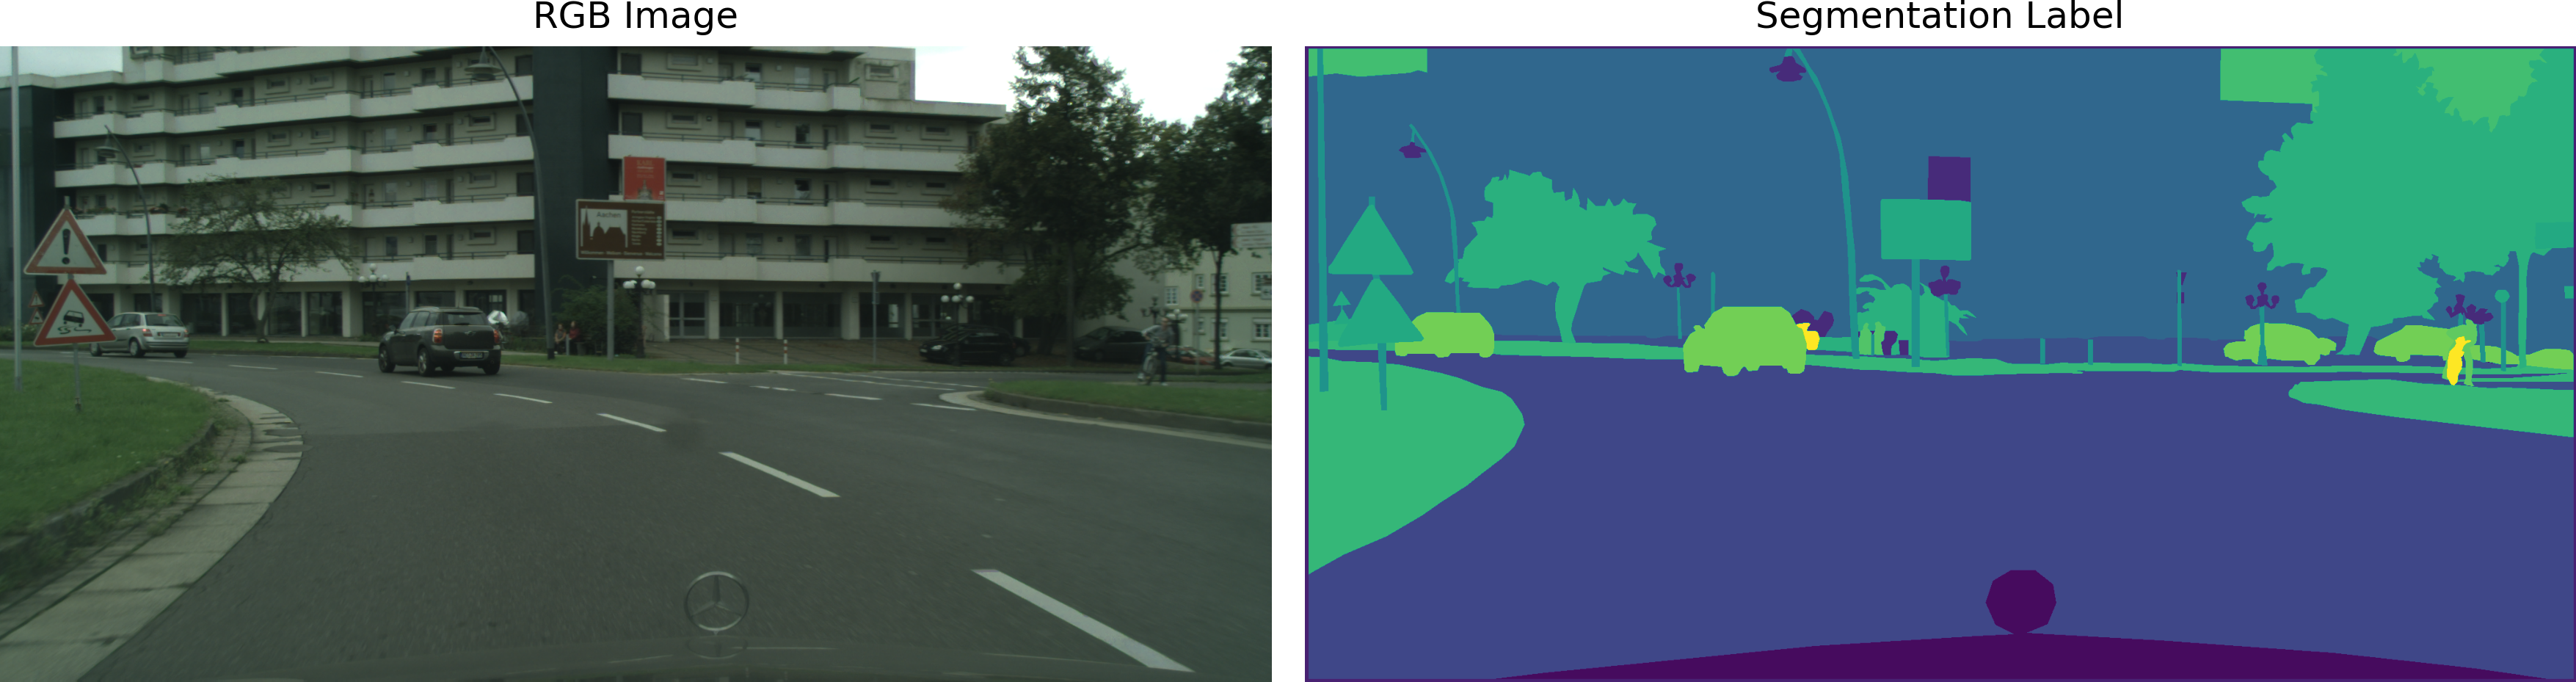
\includegraphics[scale=0.49]{pictures/output_plot_0.png}
            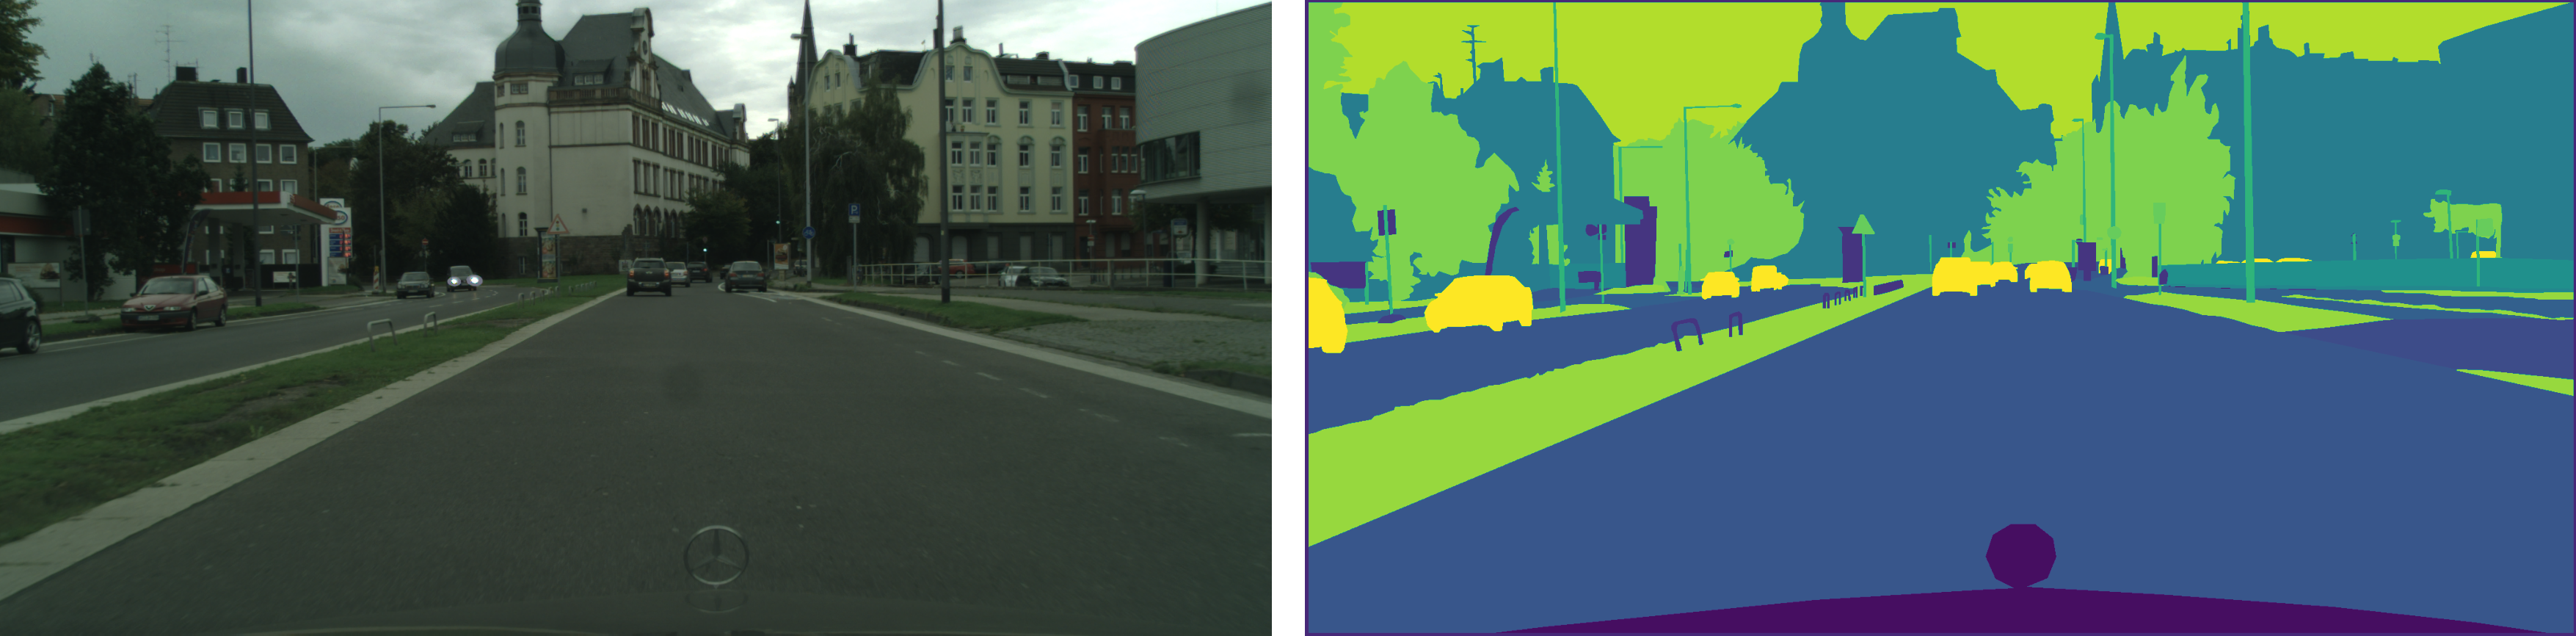
\includegraphics[scale=0.49]{pictures/output_plot_1.png}
           \caption{Die ersten zwei Bilder des Cityscapes-Datensatz aus Aachen.}
        \end{figure}

\newpage
        \subsection{Aufbau des Datensatzes}
            Der Datensatz besteht aus Bildern urbaner Szenen, aufgenommen aus $50$ verschiedenen europäischen Städten.
            Die Daten wurden mit Dashcams erfasst, die an Fahrzeugen angebracht waren. Die Bilder sind in RGB mit einer Auflösung von 2k $(2048 \times 1024)$ und haben den sogenannten Shape $(3, 2048, 1024)$. Sie liegen als verlustfreie PNG-Dateien vor.
            Diese sind in drei Kategorien unterteilt, jeweils mit entsprechenden Labels. Insgesamt umfasst der Datensatz $5000$ hochqualitative Pixel-Level-Annotationen, davon $2975$ für das Training, $500$ für die Validierung und $1525$ für den Test. Zudem enthält der Datensatz $20.000$ grob annotierte Bilder.\newline
      
            Die Labels sind in $8$ Kategorien unterteilt, mit insgesamt $30$ Klassen. Der Fokus liegt auf dem Straßenverkehr, einschließlich Autos, Fußgängern, Gebäuden und der Infrastruktur \cite{cityscapes_overview, cityscapes_paper}. 
            \begin{enumerate}
            \item \textbf{Fläche (Flat):}
                \begin{itemize}
                    \item Straße (road)
                    \item Gehweg (sidewalk)
                    \item Parkplatz (parking)
                    \item Schienenstrang (rail track)
                \end{itemize}
                \item \textbf{Menschen (human):}
                    \begin{itemize}
                    \item Fußgänger (person)
                    \item Fahrradfahrer (rider)
                \end{itemize}
                \item \textbf{Fahrzeuge (Vehicle):}
                \begin{itemize}
                    \item Auto (car)
                    \item Motorrad (motorcycle)
                    \item Fahrrad (bicycle)
                    \item Bus (bus)
                    \item LKW (truck)
                    \item Wohnmobil (caravan)
                    \item Schienenfahrzeuge (on rails)
                    \item Anhänger (trailer)
                \end{itemize}

\newpage
                \item \textbf{Konstruktionen (Construction):}
                \begin{itemize}
                    \item Gebäude (building)
                    \item Mauer (wall)
                    \item Zaun (fence)
                    \item Brücke (bridge)
                    \item Tunnel (tunnel)
                    \item Schutzgeländer (guard rail)
                \end{itemize}
                \item \textbf{Objekte (object):}
                \begin{itemize}
                    \item Polster (pole)
                    \item Ampelmasten (polegroup)
                    \item Ampel (traffic light)
                    \item Verkehrsschild (traffic sign)
                \end{itemize}
                \item \textbf{Natur (nature):}
                \begin{itemize}
                    \item Vegetation (vegetation)
                    \item Terrain (terrain)
                \end{itemize}
                \item \textbf{Himmel (sky):}
                \begin{itemize}
                    \item Himmel (sky)
                \end{itemize}
                \item \textbf{Leer (void):}
                \begin{itemize}
                    \item Alle anderen Strukturen (ground)
                    \item Temporäre Dinge (dynamic)
                    \item Hintergrund, andere Objekte (static)
                \end{itemize}
            \end{enumerate}

            Die vorhandenen Labels werden jedoch \textbf{nicht} verwendet, da für diese Arbeit eigene Labels mithilfe eines vortrainierten Modells erzeugt werden, um als Ground-Truth-Daten zu dienen.

\newpage 
    \section{Vergleich der Bilder}
        \subsection{JPEG-komprimierte Bilder}
            Die Problemdomäne dieser Arbeit ist die Reduzierung von Bilddaten, um diese im Kontext des autonomen Fahrens effizient in die Cloud hochladen und dort rekonstruieren zu können.

            Bei traditionellen Kompressionsverfahren entfällt der Teil der Rekonstruktion. Hierbei wird das Bild lediglich räumlich reduziert. Eines der bekanntesten verlustbehafteten Kompressionsverfahren ist das JPEG-Format. 
        
            Zunächst werden die Originalbilder in JPEG-Datensätze mit verschiedenen\\
            Kompressionsstufen dupliziert. Ziel ist es, die unterschiedlichen JPEG-Datensätze sowohl untereinander als auch im Vergleich zu den Originaldaten zu untersuchen. Hierfür werden die drei Metriken SSIM, PSNR und MSE angewendet. Da JPEG ein verlustbehaftetes Kompressionsverfahren ist, erfolgt die räumliche Reduzierung der Bilder auf Kosten ihrer Qualität.
            Der Faktor der Kompressionsqualität kann vom Anwender festgelegt werden und wird prozentual angegeben.
            Eine Kompressionsqualität von $100\%$ entspricht nahezu dem Original, ist jedoch ebenfalls verlustbehaftet, wie in Abbildung \ref{fig:og_hundred} zu sehen ist.
            Eine niedrigere Kompressionsqualität, beispielsweise $20\%$, führt zu deutlich sichtbaren Qualitätsverlusten, spart jedoch erheblich mehr Speicherplatz. Je geringer die Kompressionsqualität, desto ausgeprägter sind die Artefakte, die bei stark komprimierten Bildern auftreten.
               
            In dieser Arbeit wurden mittels JPEG-Kompression 15 neue Datensätze unterschiedlicher Kompressionsqualitäten (in \%) erzeugt. Diese basieren auf dem original im PNG-Format vorliegenden Datensatz, der aus den 2975 hochauflösenden
            2K-RGB-Bildern besteht.\newline
            \[
            \begin{array}{|p{0.5cm}|p{0.5cm}|p{0.5cm}|p{0.5cm}|p{0.5cm}|p{0.5cm}|p{0.5cm}|p{0.5cm}|p{0.5cm}|p{0.5cm}|p{0.5cm}|p{0.5cm}|p{0.5cm}|p{0.5cm}|p{0.5cm}|} \hline \scriptsize 5 & \scriptsize 10 & \scriptsize 15 & \scriptsize 20 & \scriptsize 25 & \scriptsize 30 & \scriptsize 40 & \scriptsize 50 & \scriptsize 60 & \scriptsize 70 & \scriptsize 75 & \scriptsize 85 & \scriptsize 90 & \scriptsize 95 & \scriptsize 100 \\ \hline \end{array}
            \]
            Dabei zeigte sich, dass die prozentuale Dateigröße im Vergleich zum Original \textbf{nicht linear} von der Kompressionsqualität abhängt.

\newpage 
            \underline{\textbf{Kompression in Bezug auf den Speicherbedarf}}        
            \begin{figure}[!htb]
                \centering
                \includesvg[scale=0.56]{graphs/output_plot_size_images.svg}
                \caption{Diese Grafik zeigt den Speicherplatz Bedarf der einzelnen Datensätze entsprechender Kompressionsqualitäten in $\%$, im Vergleich zum Originaldatensatz.}
                \label{fig:speicher_kompressionsqualität}
            \end{figure}

            Je geringer die Kompressionsqualität, desto kleiner wird die Bildgröße, was Speicherplatz spart. Dabei zeigt sich, dass der größte Unterschied der Speichergröße sich im Bereich von $95\%$ und $100\%$ Kompressionsqualität abspielt mit einer Differenz von bis zu $29,5\%$. Zwischen $85\%$ und $100\%$ sind es $39,6\%$. Mit abnehmender Kompressionsqualität sinken die Dateigrößen also drastisch ab, bis zu $85\%$ Kompressionsqualität ist dies am deutlichsten zu sehen. Unterhalb flacht die Kurve ab. Unter $70\%$ macht die Kompressionsqualität kaum noch einen Unterschied hinsichtlich des Speicherbedarfs.
            Von $5\%$ bis zu $70\%$ Kompressionsqualität gibt es über $65$ Einheiten hinweg lediglich einen Unterschied in der Dateigröße von gerade einmal $4,8\%$ Differenz. Wenn man dies im Vergleich mit der Differenz zwischen $85\%$ bis $100\%$, welche sich über $15$ Einheiten erstreckt, so ist diese um ein achtfaches kleiner auf mehr als viermal so vielen Einheiten hinweg. Die Standardabweichung (helle Schattierung) zeigt, dass die Varianz in der Dateigröße bei niedriger Kompressionsqualität sehr gering ist, aber mit steigender Qualität zunimmt. Dies könnte auf unterschiedliche Bildinhalte und die ineffiziente Speicherung bei hohen Qualitätsstufen hinweisen.

\newpage
            Die obige Grafik (Abbildung \ref{fig:speicher_kompressionsqualität}) zeigt jedoch nur das Verhältnis zwischen der Kompressionsqualität und der prozentualen Größe des Bildes auf dem Datenträger im Vergleich zum Originaldatensatz. Sie gibt jedoch noch keine Auskunft über den genauen Kompressionsfaktor. Dieser spielt eine wichtige Rolle, da er möglichst groß sein sollte, ohne die Qualität des Bildes zu sehr zu beeinträchtigen.
            
            \begin{figure}[!htb]
                \centering
                \includesvg[scale=0.56]{graphs/output_plot_ratio_images.svg}
                \caption{Diese Grafik zeigt den Kompressionsfaktor der einzelnen Datensätze entsprechend ihrer
                Kompressionsqualitäten in $\%$}
                \label{fig:speicher_kompressionsfaktor}
            \end{figure}

            Man erkennt, dass der Kompressionsfaktor mit steigender Kompressionsqualität sinkt. Höhere Qualitätsstufen weisen weniger Kompression auf und somit werden größere Dateien erzeugt. Die Funktion besitzt einen Wendepunkt bei etwa $50\%$ 
            Kompressionsqualität. Zu Beginn, in den höheren Bereichen der Kompressionsqualität, von $75\%$ bis $100\%$ ist der Kompressionsfaktor gering, jedoch stärker abfallend um eine Differenz von $11,66$. Im Vergleich zu $50\%$ bis $75\%$ beträgt die Differenz nur $6,88$. Das Gleiche lässt sich bei Kompressionsqualitäten unterhalb des Wendepunkts beobachten. Während bei Werten von $25\%$ bis $50\%$ die Differenz kleiner ist als zwischen $5\%$ und $25\%$. Die Bereiche zwischen $60\%$ und $75\%$ können als der „Sweetspot“ angesehen werden, um einen guten Kompressionsfaktor und reduzierten Speicherbedarf zu erreichen bei Kompressionsqualitäten oberhalb des Wendepunkts.
            Die Grafik weist Ähnlichkeiten mit der der Funktion aus Abbildung \ref{fig:speicher_kompressionsqualität} auf, bei der ebenfalls ein minimaler Wendepunkt bei $50\%$ erkennbar ist.
            
\newpage  
            \underline{\textbf{Qualität der Bilder}}\bigskip

            \textbf{Kompressionsqualität (40)}
            \begin{figure}[!htb]
                \centering
                \begin{minipage}[!htb]{0.47\textwidth}
                    \centering
                    \textbf{Komprimiert} % Überschrift für die erste Spalte
                \end{minipage}
                %
                \begin{minipage}[!htb]{0.47\textwidth}
                    \centering
                    \textbf{Original} % Überschrift für die zweite Spalte
                \end{minipage}

                \begin{minipage}[!htb]{0.47\textwidth}
                    \centering
                    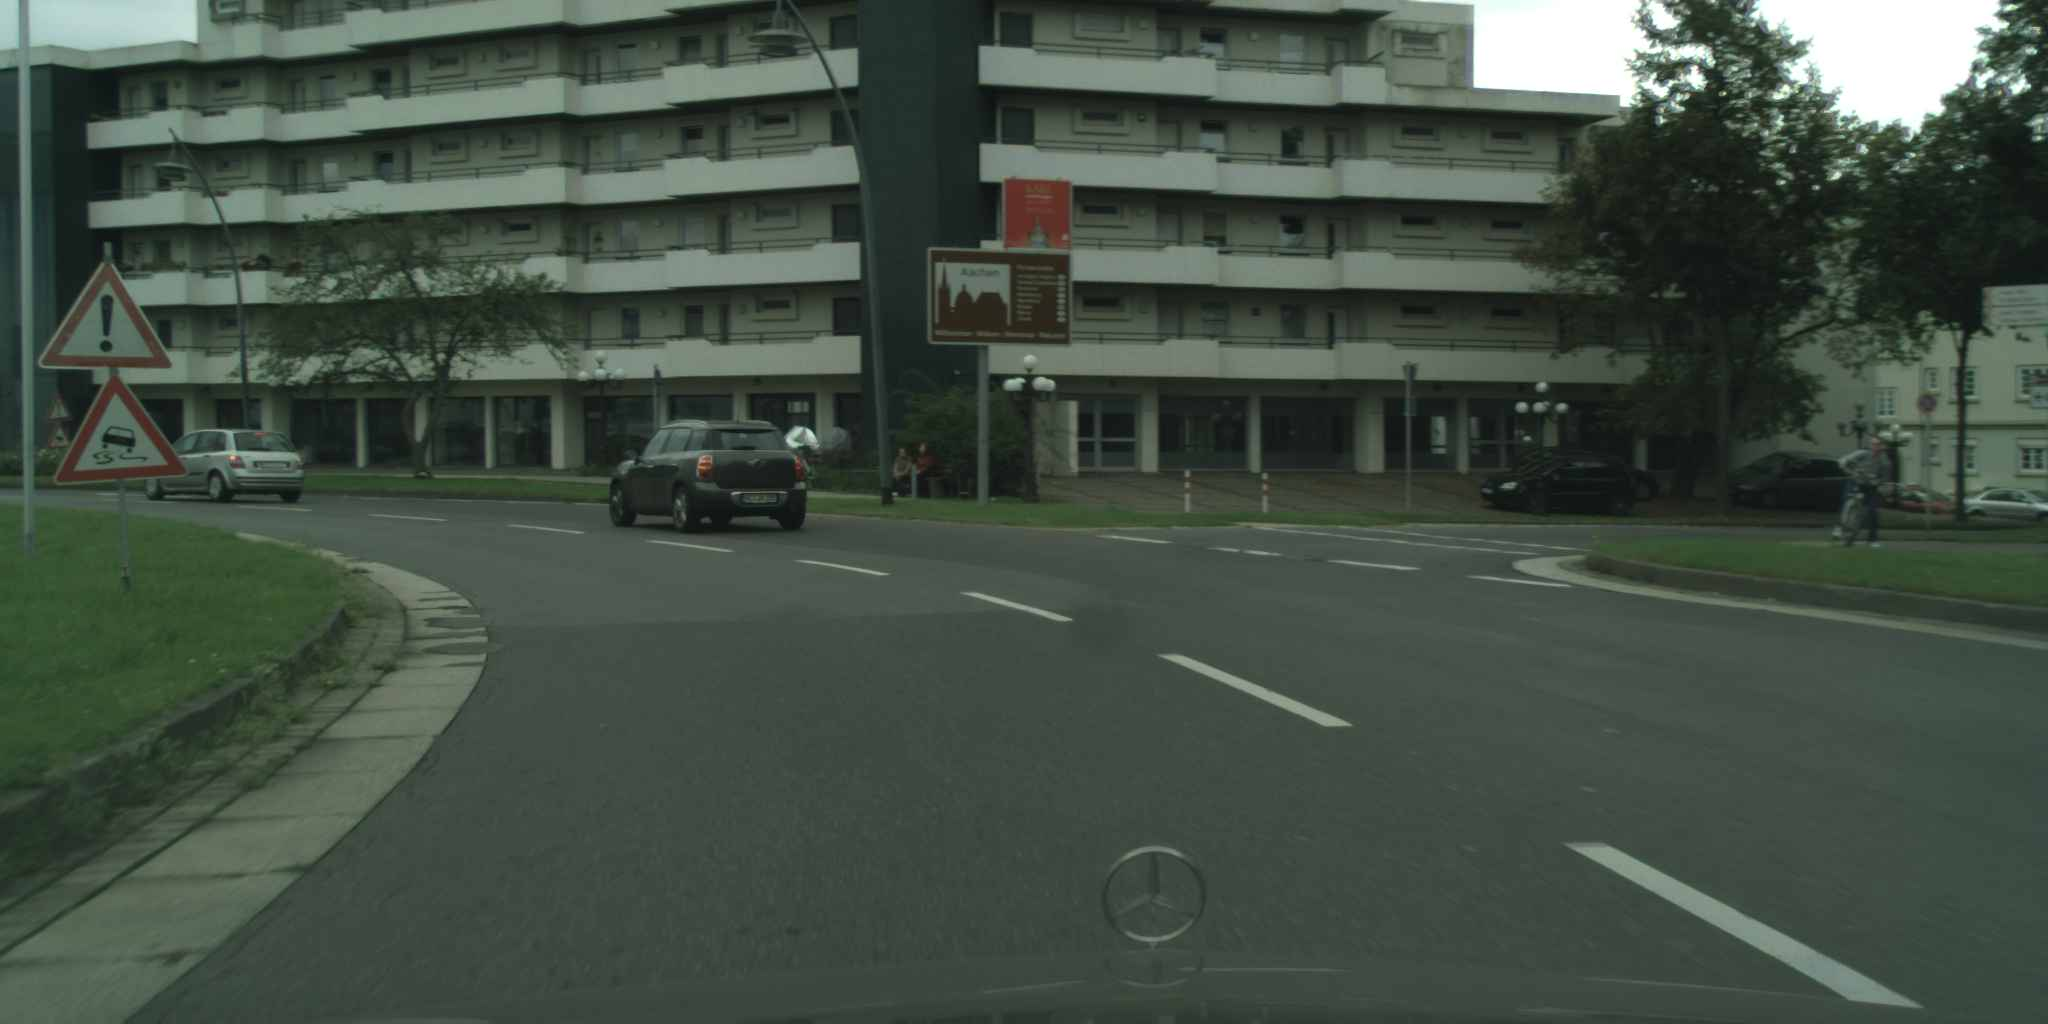
\includegraphics[width=\textwidth]{pictures/img00_jpg_40.jpg}    
                    \label{fig:bild5}
                \end{minipage}
                %
                \begin{minipage}[!htb]{0.47\textwidth}
                    \centering
                    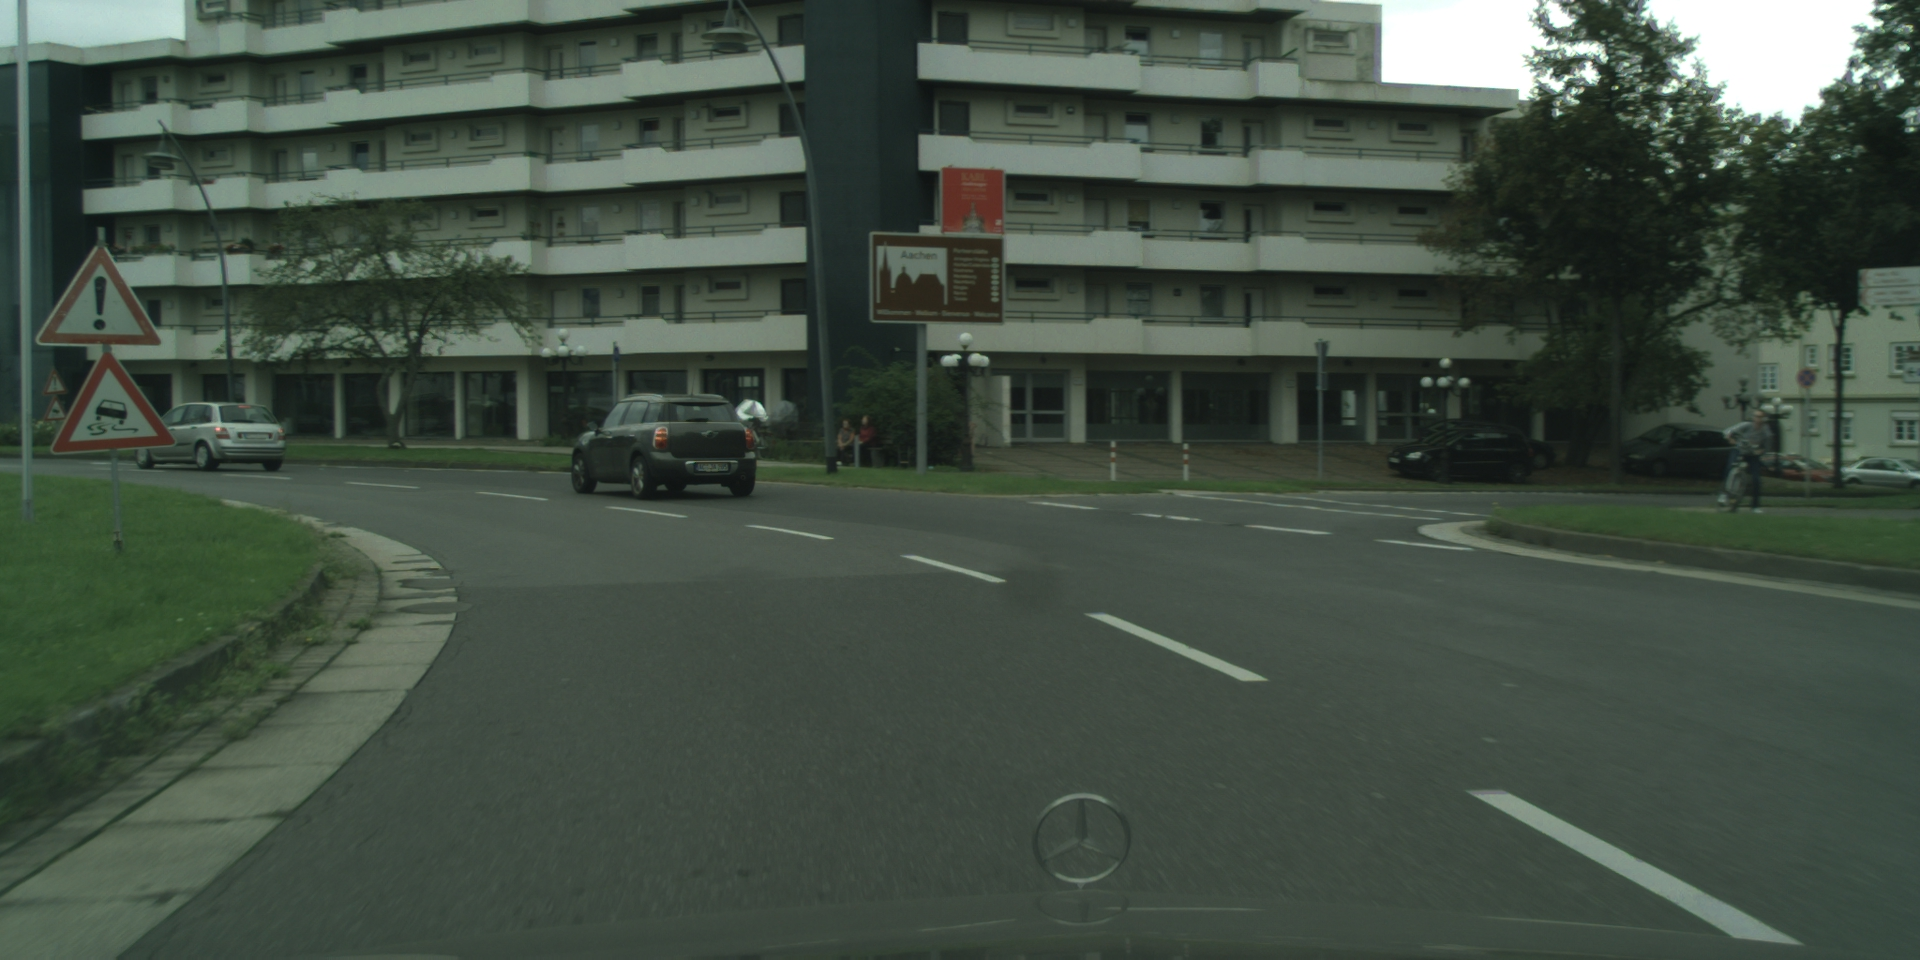
\includegraphics[width=\textwidth]{pictures/img00_png.jpg}
                    \label{fig:bild6}
                \end{minipage}
            \end{figure}
        
            \textbf{Kompressionsqualität (15)}
            \begin{figure}[!htb]
                \centering
                \begin{minipage}[!htb]{0.47\textwidth}
                    \centering
                    \textbf{Komprimiert} % Überschrift für die erste Spalte
                \end{minipage}
                %
                \begin{minipage}[!htb]{0.47\textwidth}
                    \centering
                    \textbf{Original} % Überschrift für die zweite Spalte
                \end{minipage}

                \begin{minipage}[!htb]{0.47\textwidth}
                    \centering
                    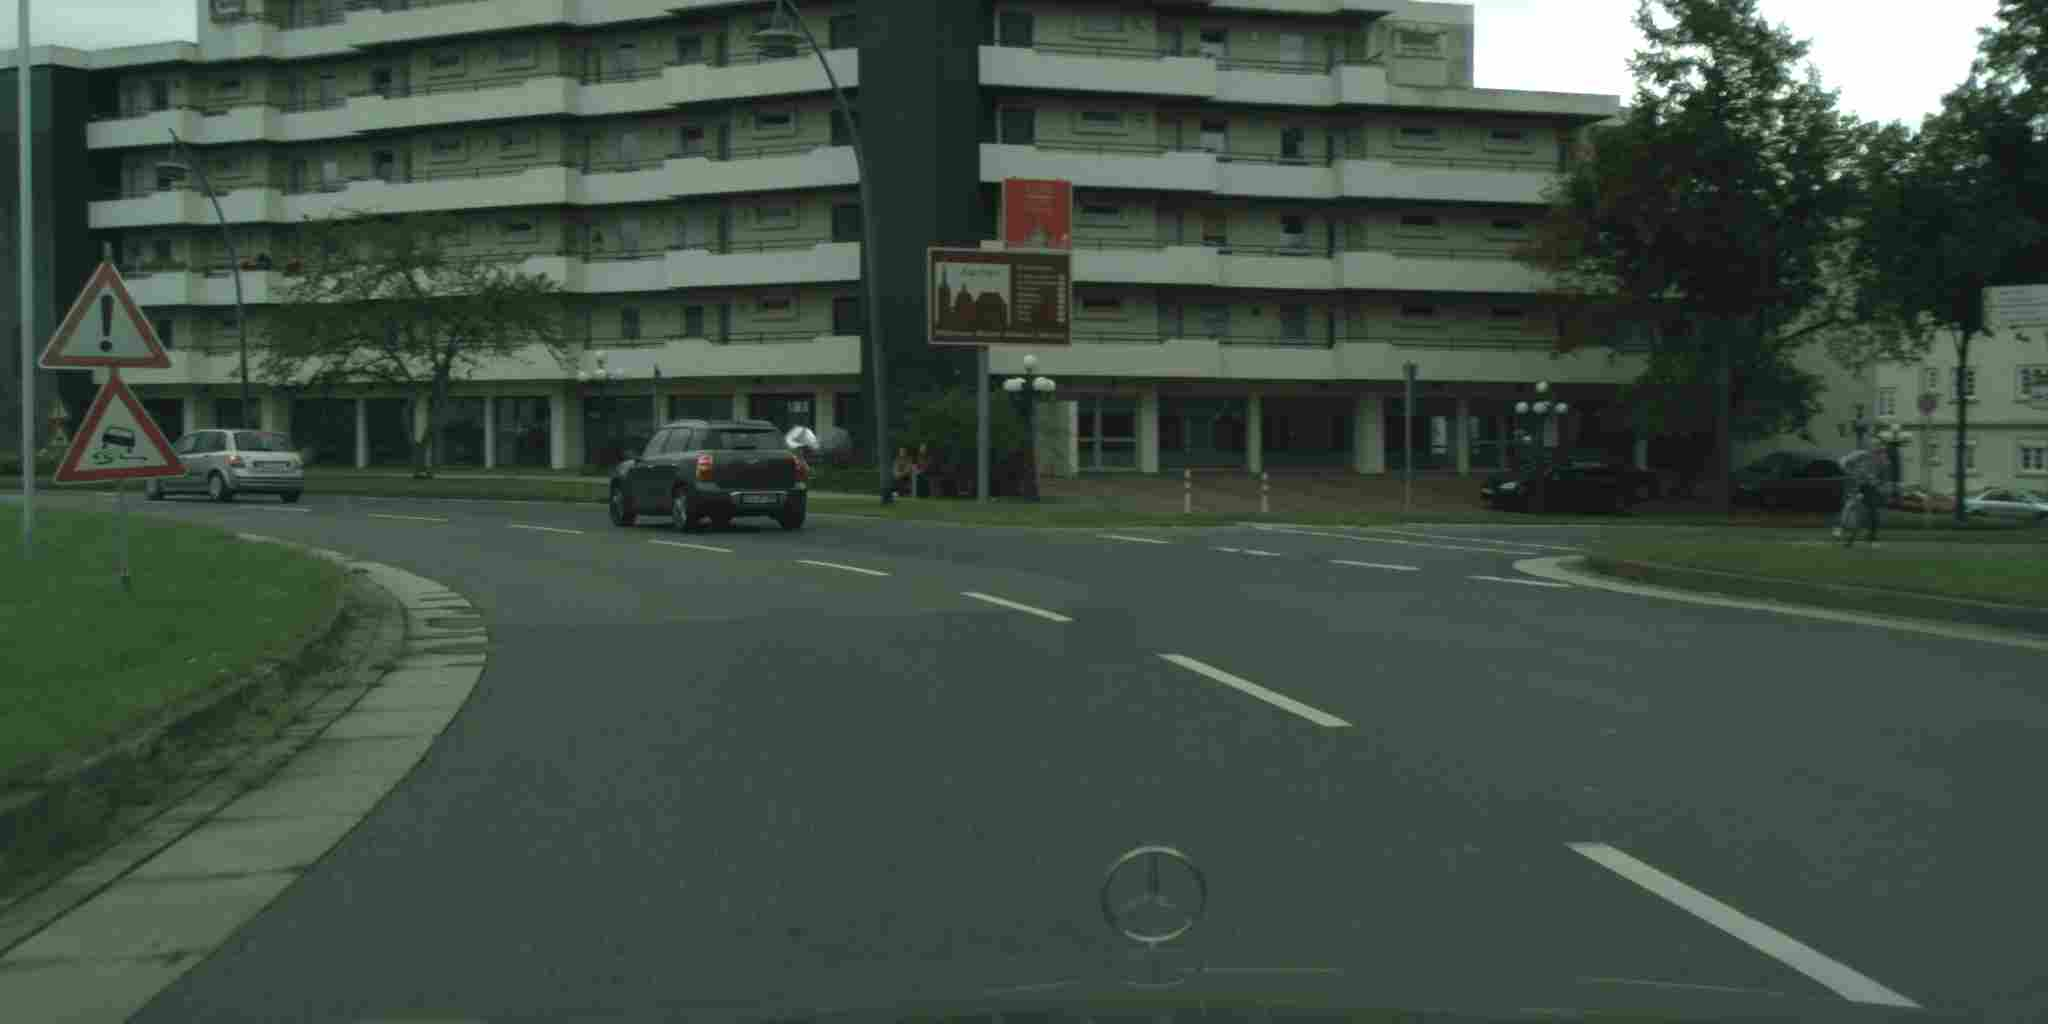
\includegraphics[width=\textwidth]{pictures/img00_jpg_15.jpg}    
                    \label{fig:bild9}
                \end{minipage}
                %
                \begin{minipage}[!htb]{0.47\textwidth}
                    \centering
                    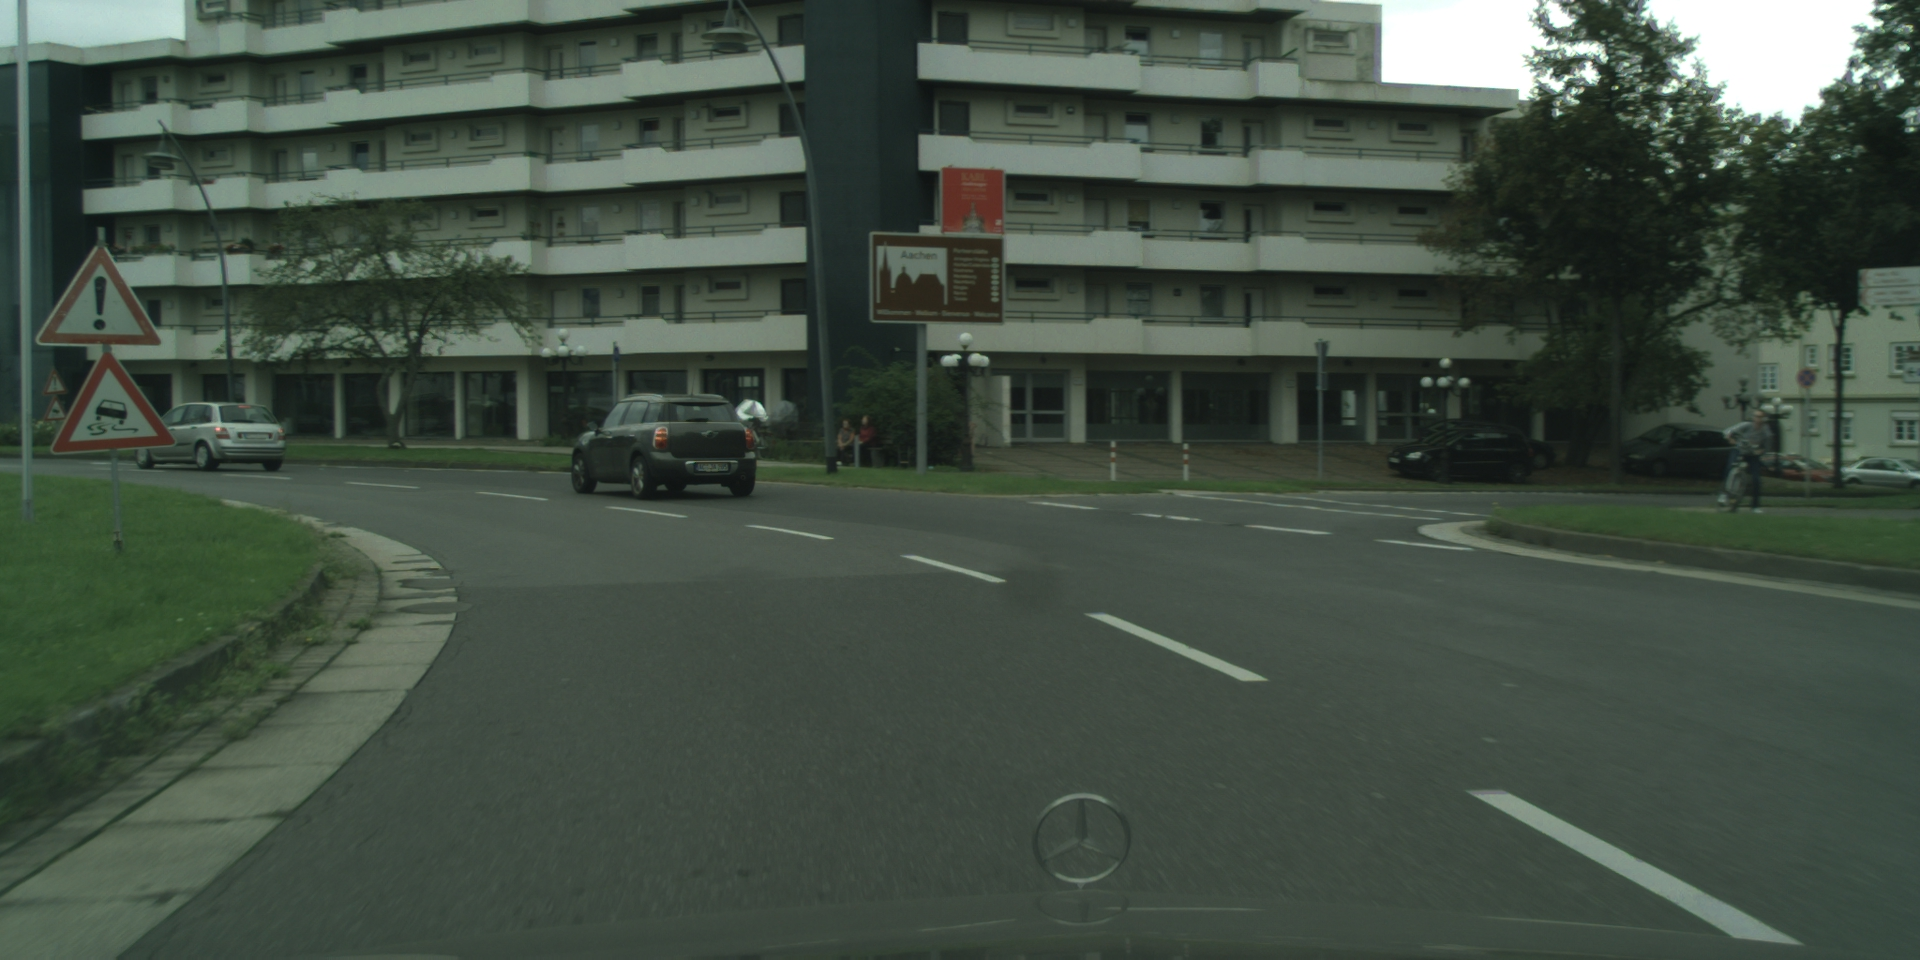
\includegraphics[width=\textwidth]{pictures/img00_png.jpg}
                    \label{fig:bild10}
                \end{minipage}
            \end{figure}

            \textbf{Kompressionsqualität (5)}
            \begin{figure}[!htb]
                \centering
                \begin{minipage}[!htb]{0.47\textwidth}
                    \centering
                    \textbf{Komprimiert} % Überschrift für die erste Spalte
                \end{minipage}
                %
                \begin{minipage}[!htb]{0.47\textwidth}
                    \centering
                    \textbf{Original} % Überschrift für die zweite Spalte
                \end{minipage}

                \begin{minipage}[!htb]{0.47\textwidth}
                    \centering
                    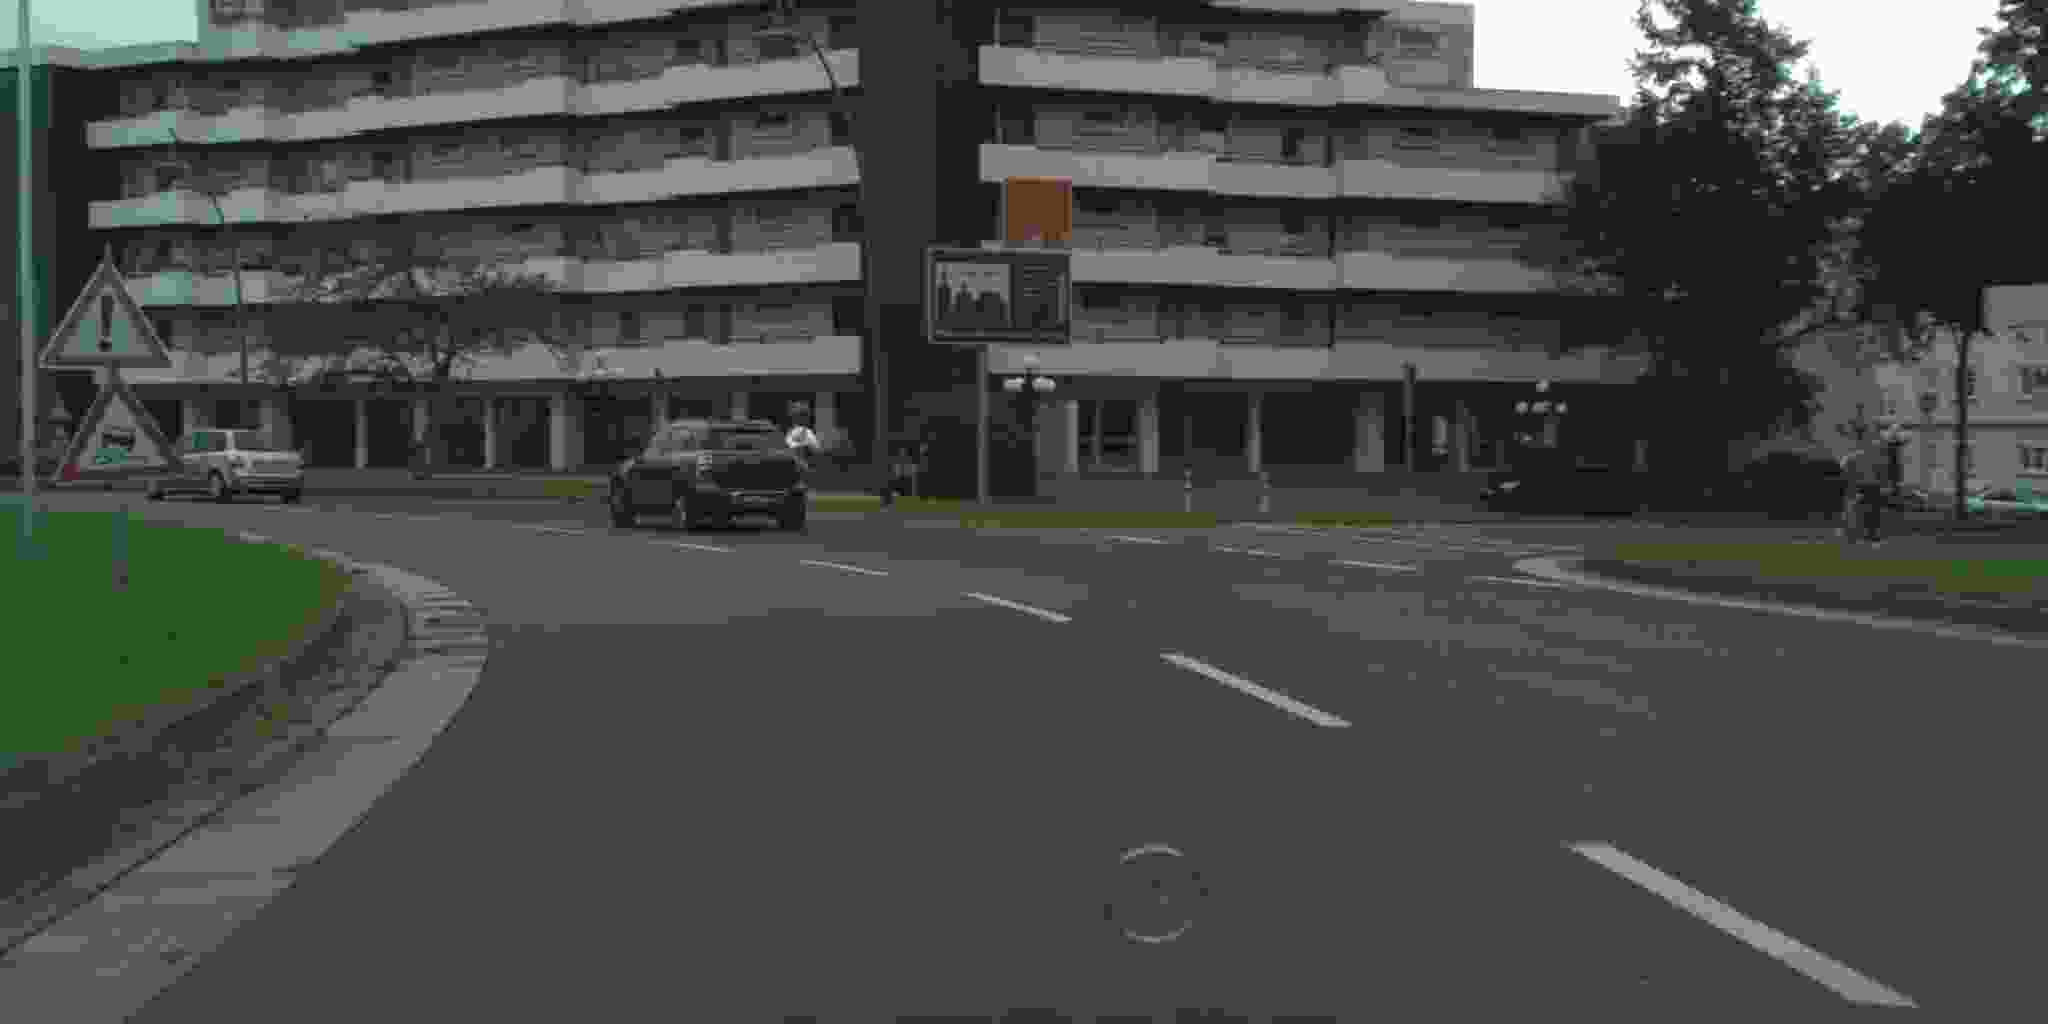
\includegraphics[width=\textwidth]{pictures/img00_jpg_5.jpg}    
                    \label{fig:bild13}
                \end{minipage}
                %
                \begin{minipage}[!htb]{0.47\textwidth}
                    \centering
                    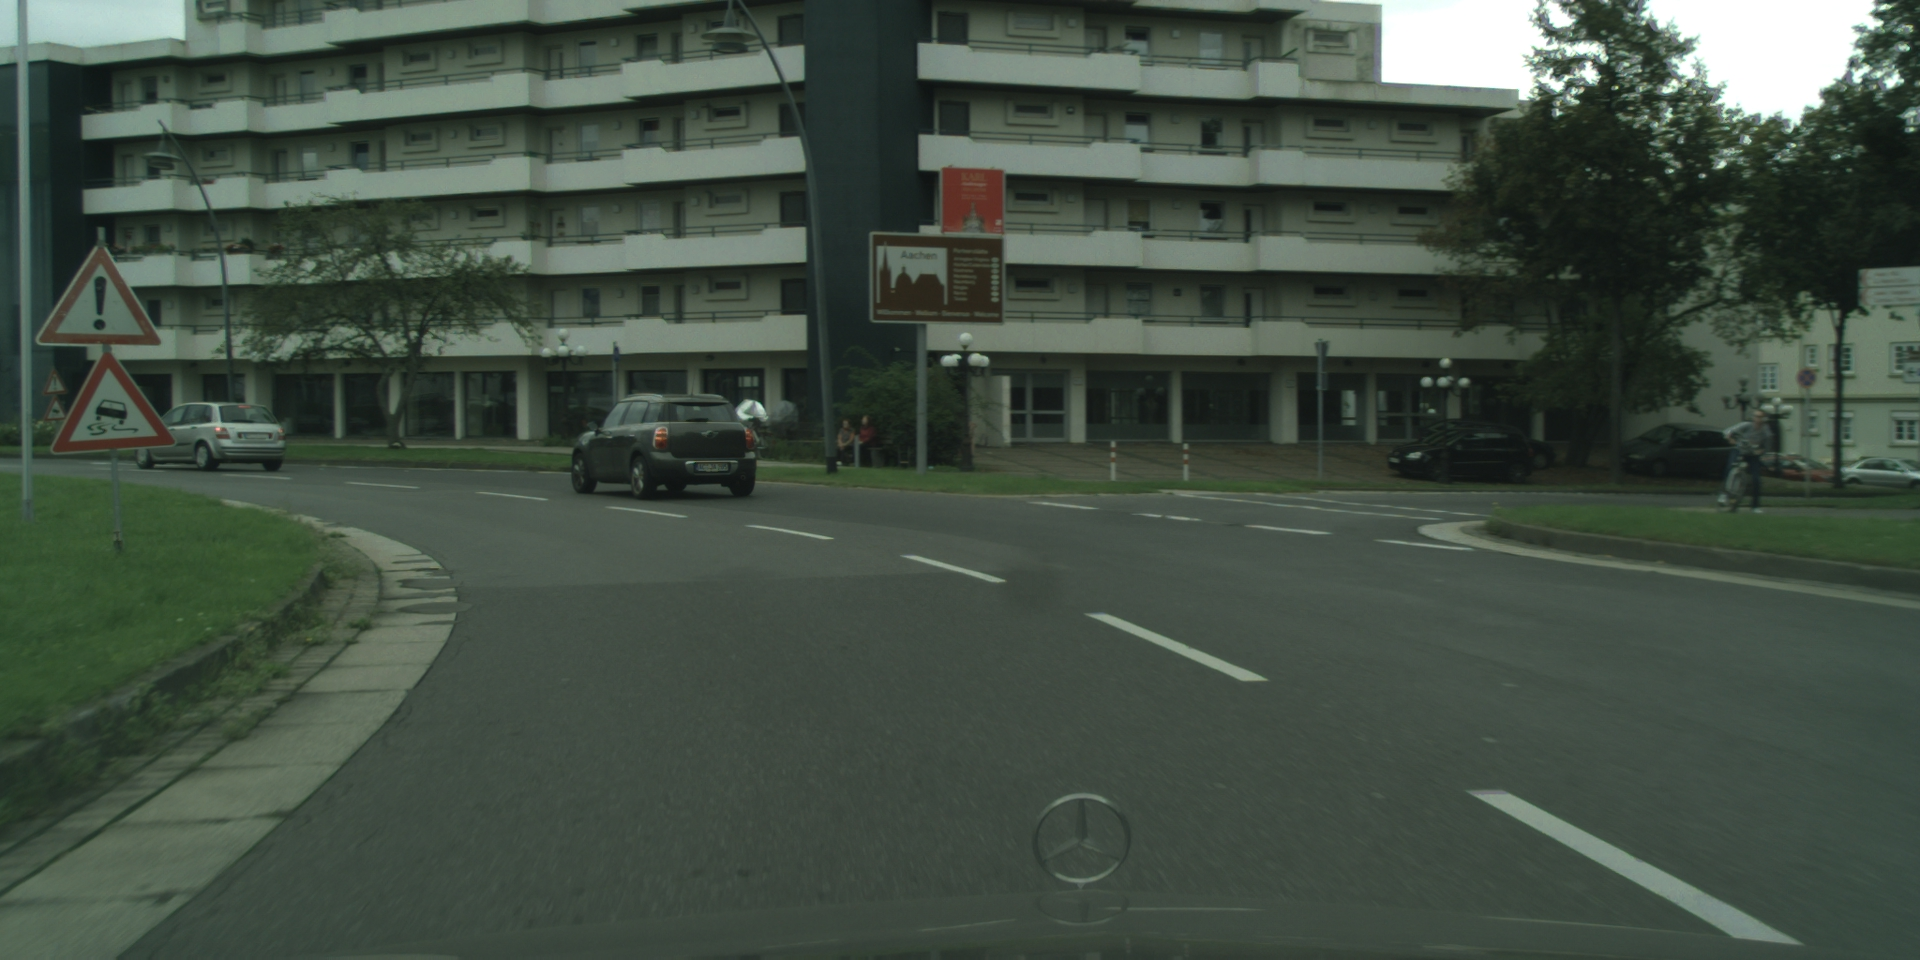
\includegraphics[width=\textwidth]{pictures/img00_png.jpg}
                    \label{fig:bild14}
                \end{minipage}
            \end{figure}

\newpage
            Interessant ist, dass sich JPEG-komprimierte Bilder anfangs kaum bis gar nicht voneinander unterscheiden, wenn man sie mit dem Original vergleicht. Erst bei einer Kompressionsqualität von etwa $15\%$ werden die Qualitätseinbußen des Bildes deutlich sichtbar. Auch bei einer Kompressionsqualität von $100\%$ ist die Bildqualität minimal schlechter als die des Originals. Dieser Unterschied ist jedoch mit dem menschlichen Auge nicht erkennbar, wie der folgende Bildvergleich zeigt.

            \begin{figure}[!htb]
                \centering
                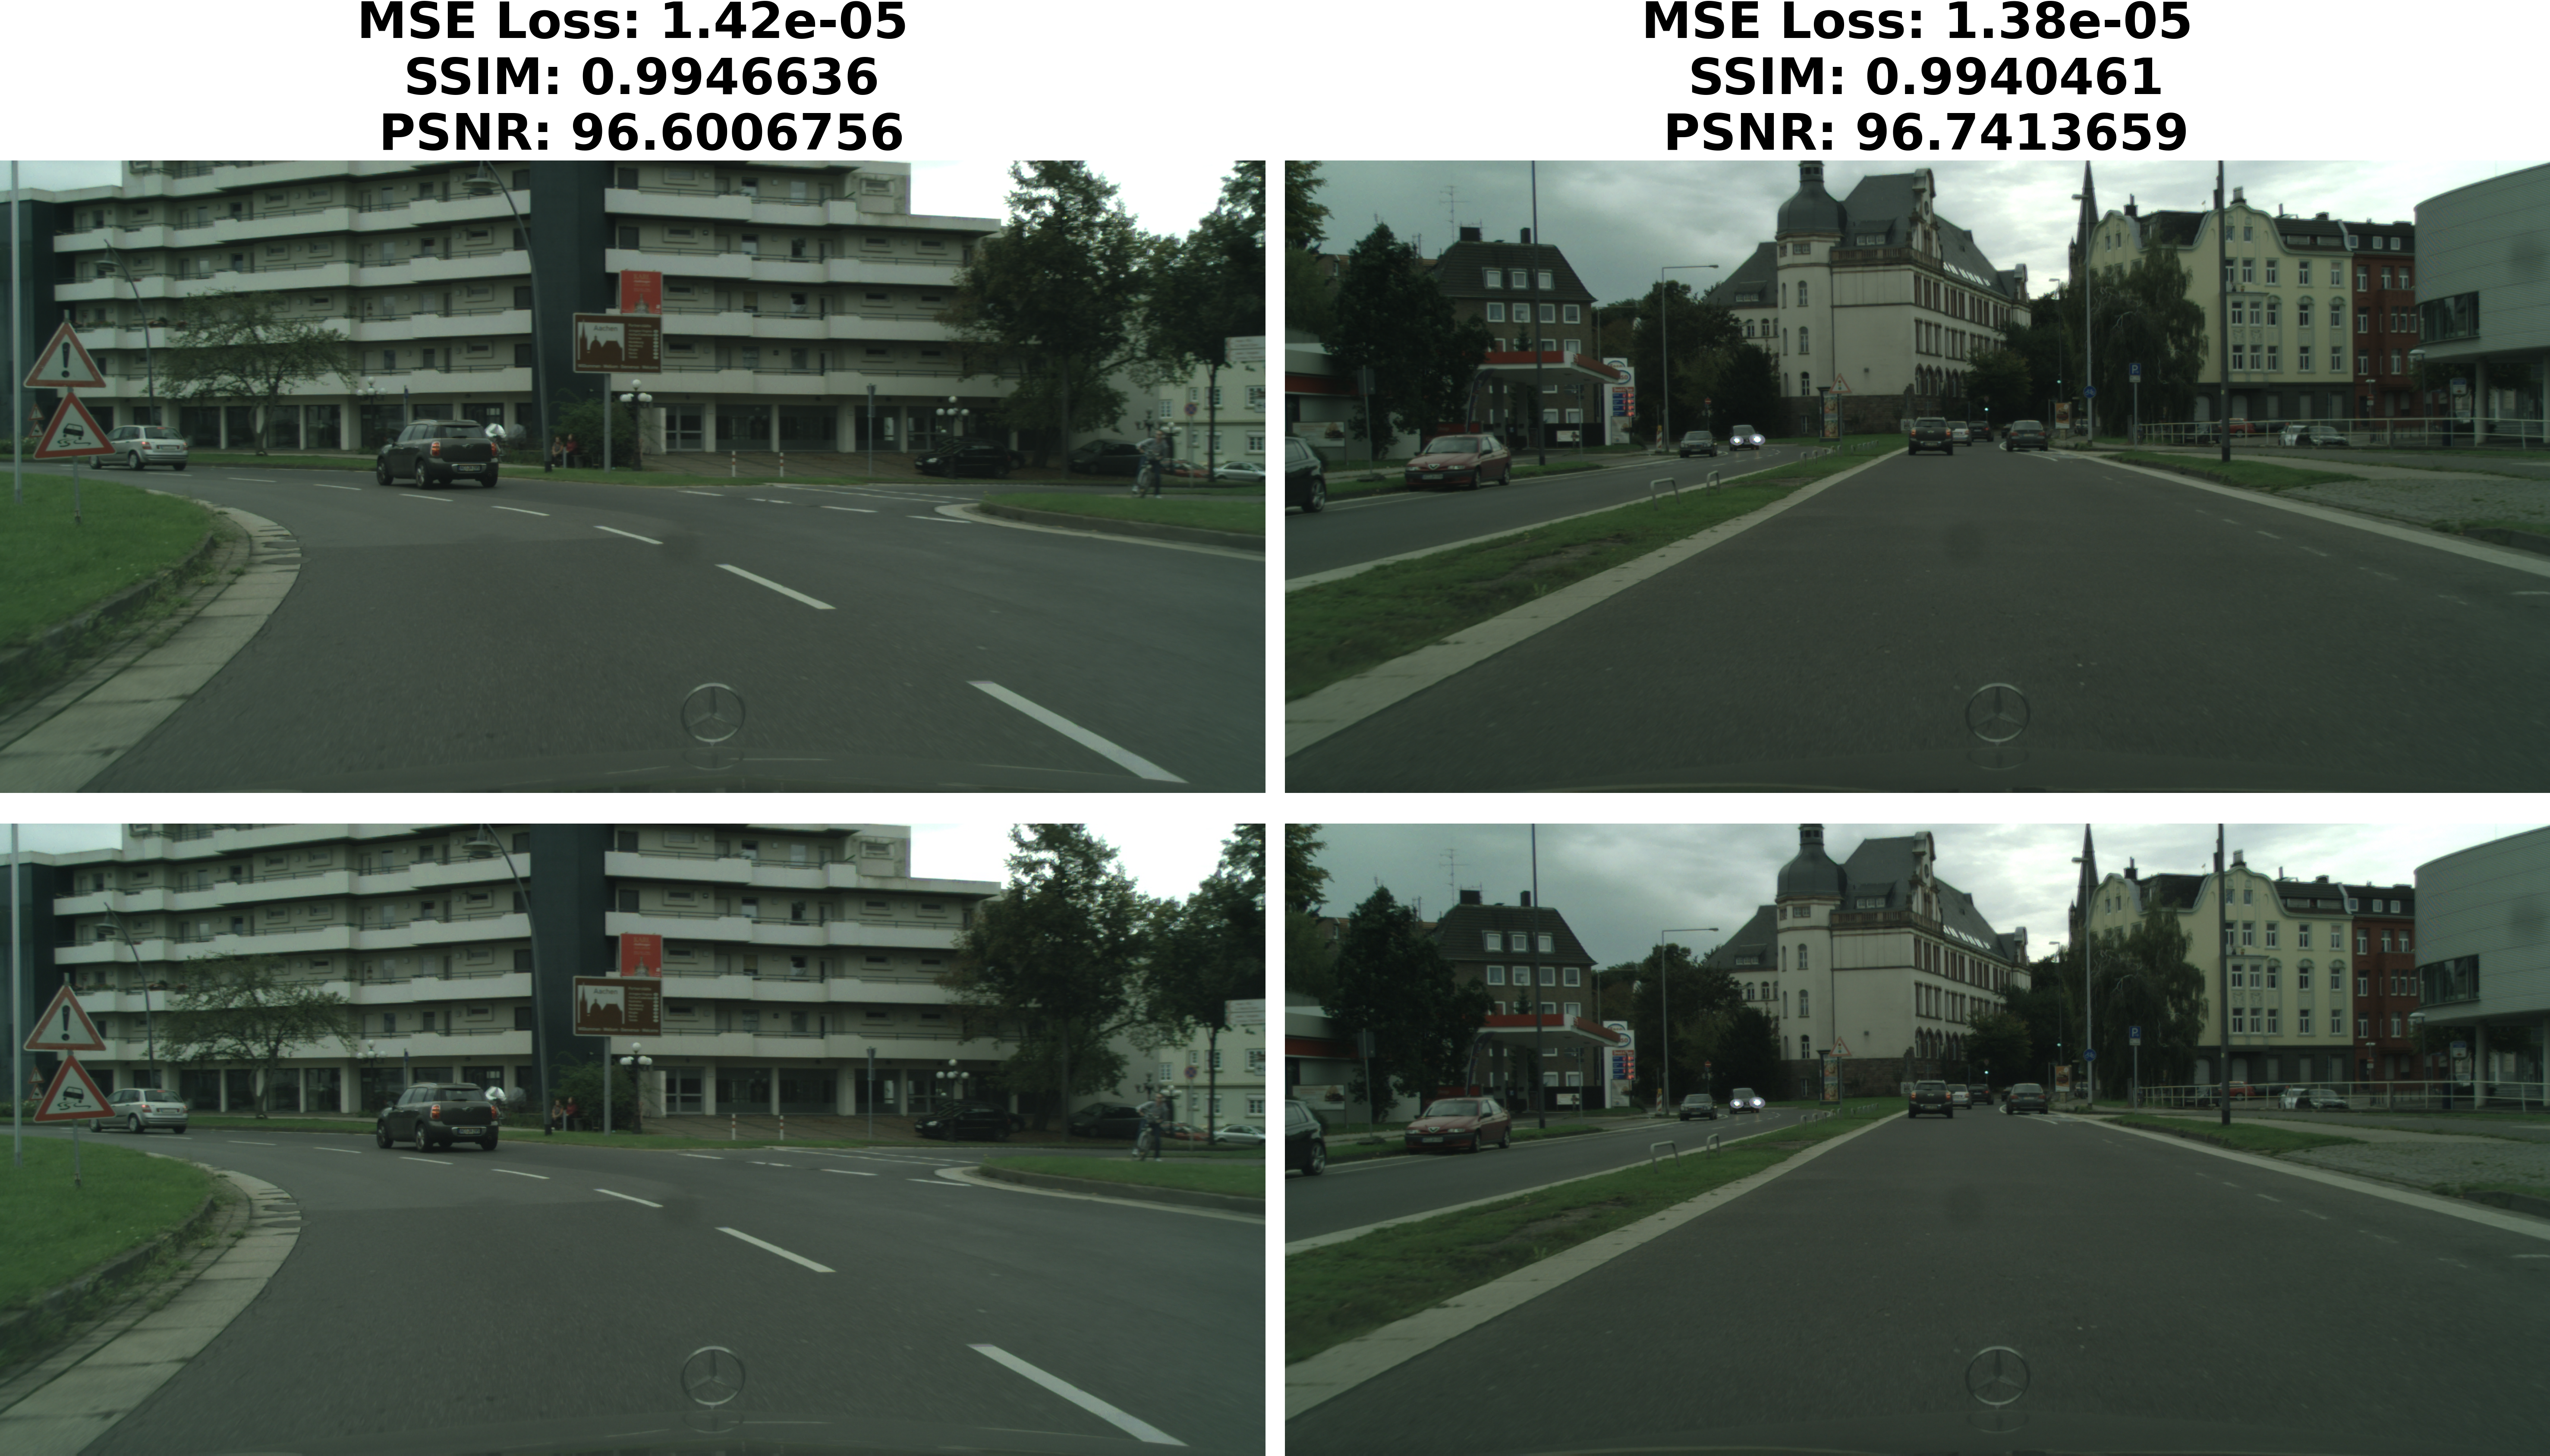
\includegraphics[scale=0.27]{pictures/output_plot_100.png}
                \caption{Oben das Original und unten das mit Kompressionsqualität von $100\%$ komprimierte JPEG-Bild.}
                \label{fig:og_hundred}
            \end{figure}

            Bei einem identischen Bild ohne Verluste würde der MSE $0.0$, der SSIM $1.0$ und der PSNR-Score $100$ betragen. Somit ist auch eine Kompressionsqualität von $100\%$ verlustbehaftet. Obwohl die Verluste verschwindend gering und mit dem menschlichen Auge nicht erkennbar sind, können sie mithilfe dieser Metriken nachgewiesen werden.\bigskip

            Die folgenden Grafiken zeigen den Qualitätsverlust, gemessen anhand von MSE, SSIM und PSNR, in Bezug auf die Kompressionsqualität in Prozent.

\newpage       
            \begin{figure}[!htb]
                \centering
                \includesvg[scale=0.56]{graphs/output_plot_mse.svg}
                \caption{Durchschnittswert MSE aller Bilder der JPEG-Datensätze.}
            \end{figure}

            \begin{figure}[!htb]
                \centering
                \includesvg[scale=0.56]{graphs/output_plot_ssim.svg}
                \caption{Durchschnittswert SSIM aller Bilder der JPEG-Datensätze.}
            \end{figure}
        
\newpage
            Die obere Grafik zeigt den MSE, die untere den SSIM. Es fällt direkt auf, dass der SSIM die Inverse zum MSE darstellt. Während der MSE mit $25\%$ einen Wert von $0,0003$ hat, steigt er unterhalb dieser Kompressionsqualität stark an auf ein sechseinhalb-faches bei $5\%$. Der SSIM hingegen, welcher sich stets von $100\%$ bis $25\%$ Kompressionsqualität in einem Wertebereich von $0,058$ bewegt hat, fällt unterhalb des Schwellenwerts von $25\%$ um ganze $0,3$ ab. Somit sollte man keine Kompressionsqualität unterhalb von $25\%$ wählen. Wie bereits in Abbildung \ref{fig:speicher_kompressionsqualität} zu sehen war, macht es für den Speicherbedarf unterhalb von $60-70\%$ keinen nennenswerten Unterschied mehr.
            
            \begin{figure}[!htb]
                \centering
                \includesvg[scale=0.56]{graphs/output_plot_psnr.svg}
                \caption{Durchschnittswert PSNR alle Bilder der JPEG-Datensätze.}
            \end{figure}

            Beim PSNR verhält es sich ähnlich wie in Abbildung \ref{fig:speicher_kompressionsfaktor}. Ein klarer Wendepunkt ist bei einer Kompressionsqualität von $50\%$ erkennbar. Oberhalb dieses Punktes fällt die Qualität von $100\%$ abwärts und flacht
            bis $50\%$ ab. Unterhalb dieses Wendepunkts fällt die Kurve bei abnehmender Kompressionsqualitäten immer stärker.      
        
            Bei Betrachtung der Grafiken und der Bilder unterschiedlicher Kompressionsqualitäten wird deutlich, warum die Bilder mit $100\%$ und $40\%$ Kompressionsqualität im Vergleich zum Original kaum voneinander zu unterscheiden waren. Die Grafiken zeigen, dass die Bildqualität erst ab einer Kompressionsqualität von $25\%$ bis $30\%$ sichtbar nachlässt.

            Eine Kompressionsqualität von ca. $80\%$ bietet einen guten Kompromiss, akzeptable Bildqualität (hohe PSNR- und SSIM-Werte) bei geringem Speicherbedarf.
            
        %\begin{figure}[!htb]
        %    \centering
        %    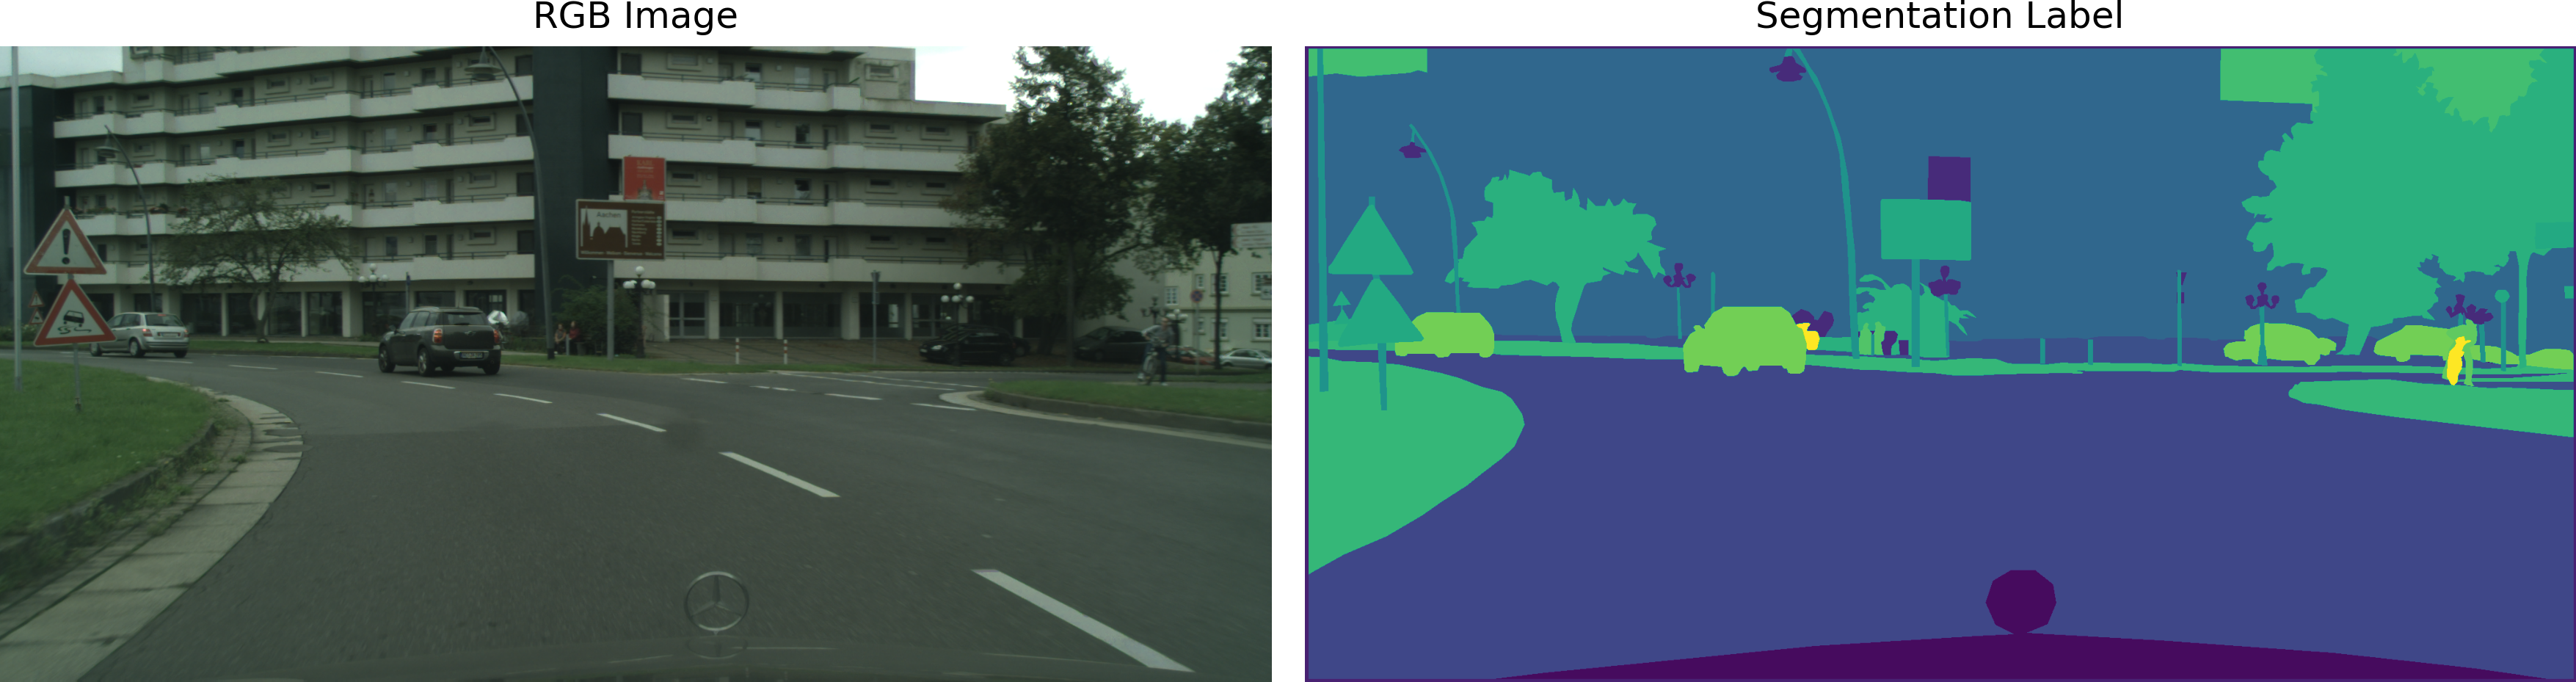
\includegraphics[scale=0.49]{pictures/output_plot_0.png}
        %    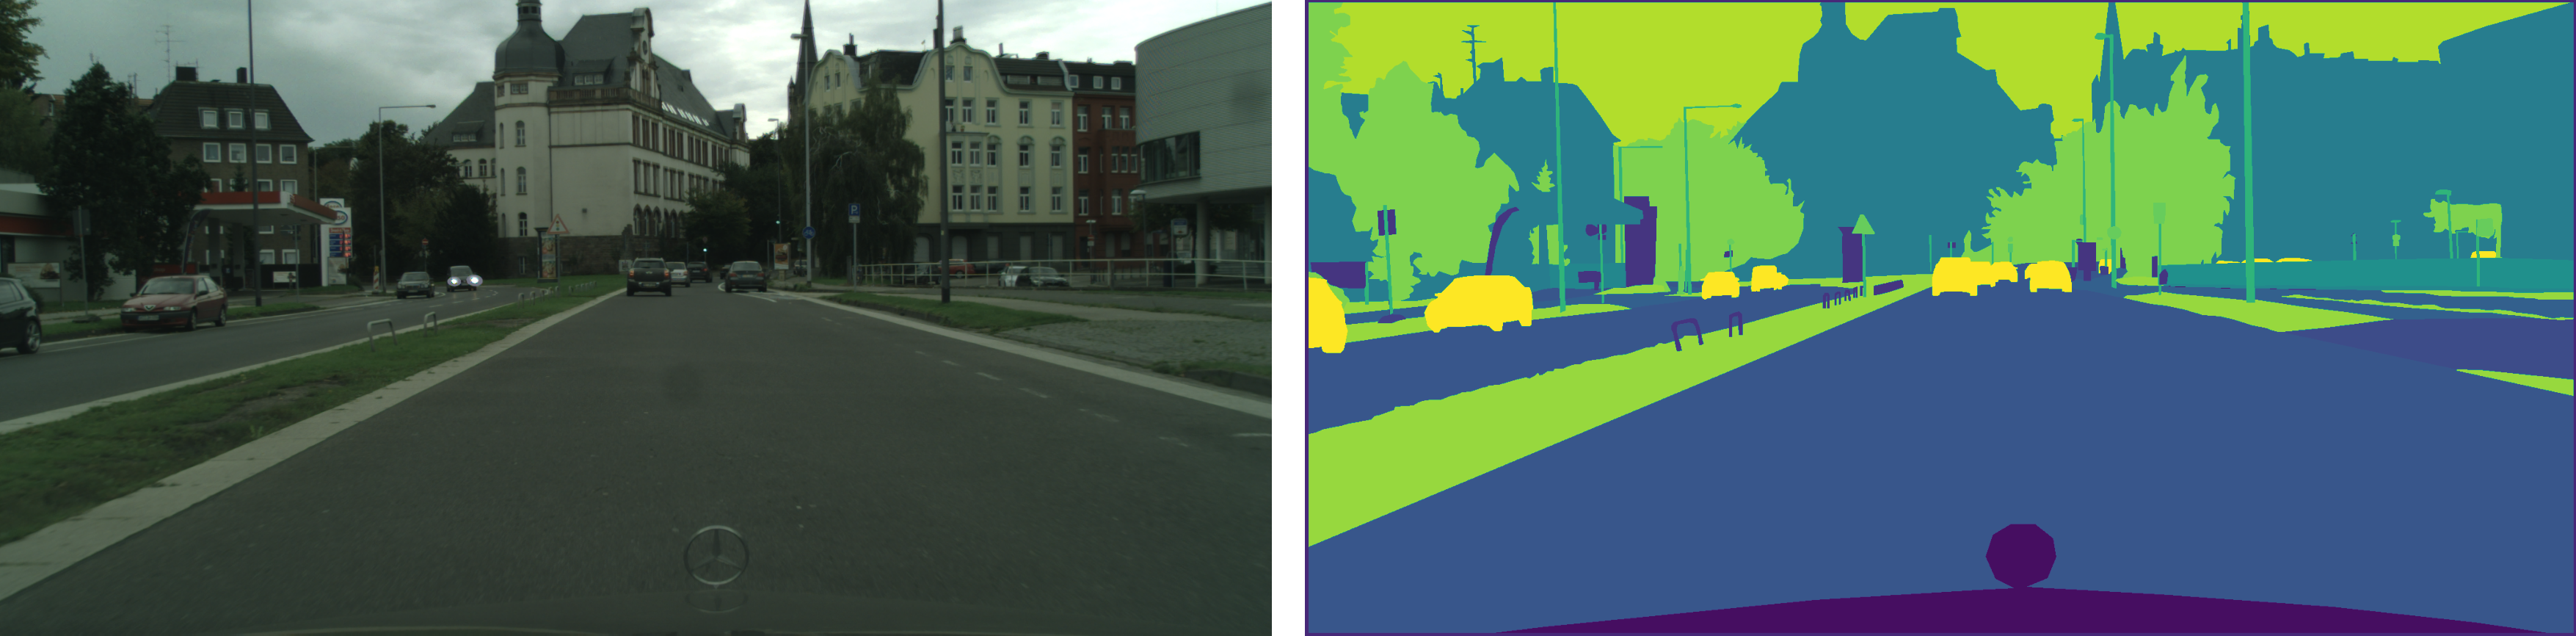
\includegraphics[scale=0.49]{pictures/output_plot_1.png}
        %    \caption{Die ersten zwei Bilder des Cityscapes Dataset aus Aachen.}
        %\end{figure}        
    
\newpage  
        \subsection{KI-rekonstruierte Bilder}
            Für die KI-rekonstruierten Bilder werden zwei VQ-VAE-Modelle verwendet, die in Kapitel 5 (Modelle) vorgestellt wurden. Anders als bei traditionellen Bildkompressionsverfahren wie JPEG wird das Bild in diesem Ansatz nicht nur komprimiert, sondern anschließend rekonstruiert. Daraus entstanden zwei neue Datensätze, die für die weiteren Untersuchungen erstellt wurden.
            
            Die beiden KI-Datensätze werden sowohl untereinander als auch zu den Originaldaten sowie zu den JPEG-Daten mithilfe der drei Metriken SSIM, PSNR und MSE untersucht.
            Anders als bei der Untersuchung von JPEG werden hier die Metriken nicht in Abhängigkeit von der Kompressionsqualität gemessen, da sich diese ausschließlich auf die JPEG-Komprimierung bezieht.
            Für den Vergleich und die Untersuchung der KI-rekonstruierten Datensätze werden die Metriken stattdessen in Abhängigkeit vom Kompressionsfaktor gemessen.

            In Abbildung \ref{fig:speicher_kompressionsfaktor} ist der Kompressionsfaktor der einzelnen
            JPEG-Datensätze in Bezug auf ihre Kompressionsqualität dargestellt. Die Kurve ist nicht linear und zeigt einen maximalen Kompressionsfaktor von $56,33$ bei einer Kompressionsqualität von $5\%$.
            Im Vergleich dazu erreichen die beiden Modelle deutlich höhere Kompressionsfaktoren.
            \begin{itemize}
                \item \textbf{vq-f16} f=16, VQ (Z=16384, d=8)\\
                    Erreicht einen Kompressionsfaktor von $219,43$
                \item \textbf{vq-f8-n256} f=8, VQ (Z=256, d=4)\\
                     Erreicht einen Kompressionsfaktor von $192$
            \end{itemize}
            Obwohl das Codebuch des \textbf{vq-f8-n256} signifikant kleiner ist und weniger Einträge enthält, um die latenten Vektoren auf die Codebuchvektoren abzubilden, und die Dimension der latenten Vektoren mit $d = 4$ ebenfalls geringer ist, erzielt das \textbf{vq-f8-n256}-Modell eine niedrigere Kompression.
            Die Zerlegung des Bildes erfolgt durch kleinere Blöcke, was einen stärkeren Einfluss darauf hat, wie stark die Kompression letztendlich ausfällt. Da die Blöcke der Größe $f \times f$ auf die Höhe und die Breite des Bildes angewandt werden, ist der Wert $f$ vierfach zu zählen im Vergleich zur Dimension $d$.
            Das bedeutet, dass für ($f = 8$, $d=4$) der gleiche latente Vektor wie für ($f=16$, $d=8$) erst dann resultieren würde, wenn ($f=8$, $d=2$) verwendet wird.

\newpage 
            \underline{\textbf{Qualität der Bilder}}\bigskip
\begin{comment}         
            Original im Vergleich zum \textbf{vq-f16} Modell      
            \begin{figure}[!htb]
                \centering
                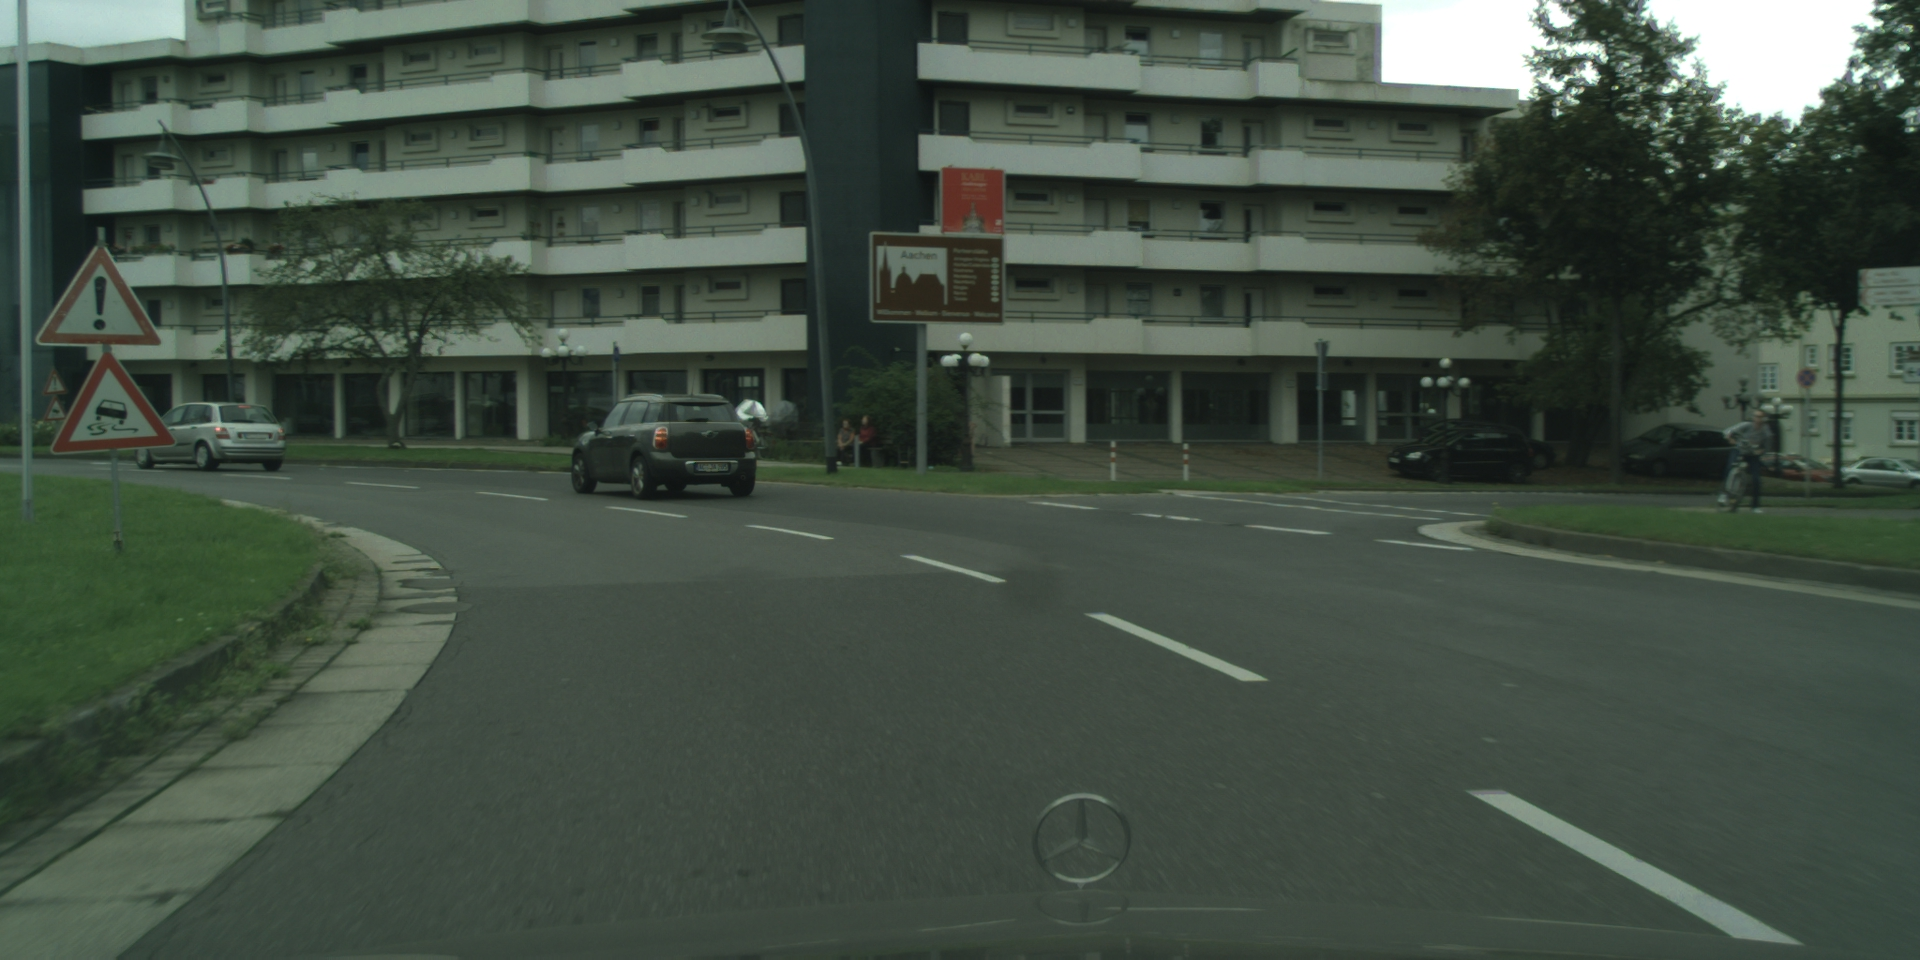
\includegraphics[scale=0.19]{pictures/img00_png.png}
                \caption{Originales Bild aus dem Cityscapes  Datensatz (Aachen erstes Bild).}
                \label{fig:og0_aachen_000000}
            \end{figure}
            \begin{figure}[!htb]
                \centering
                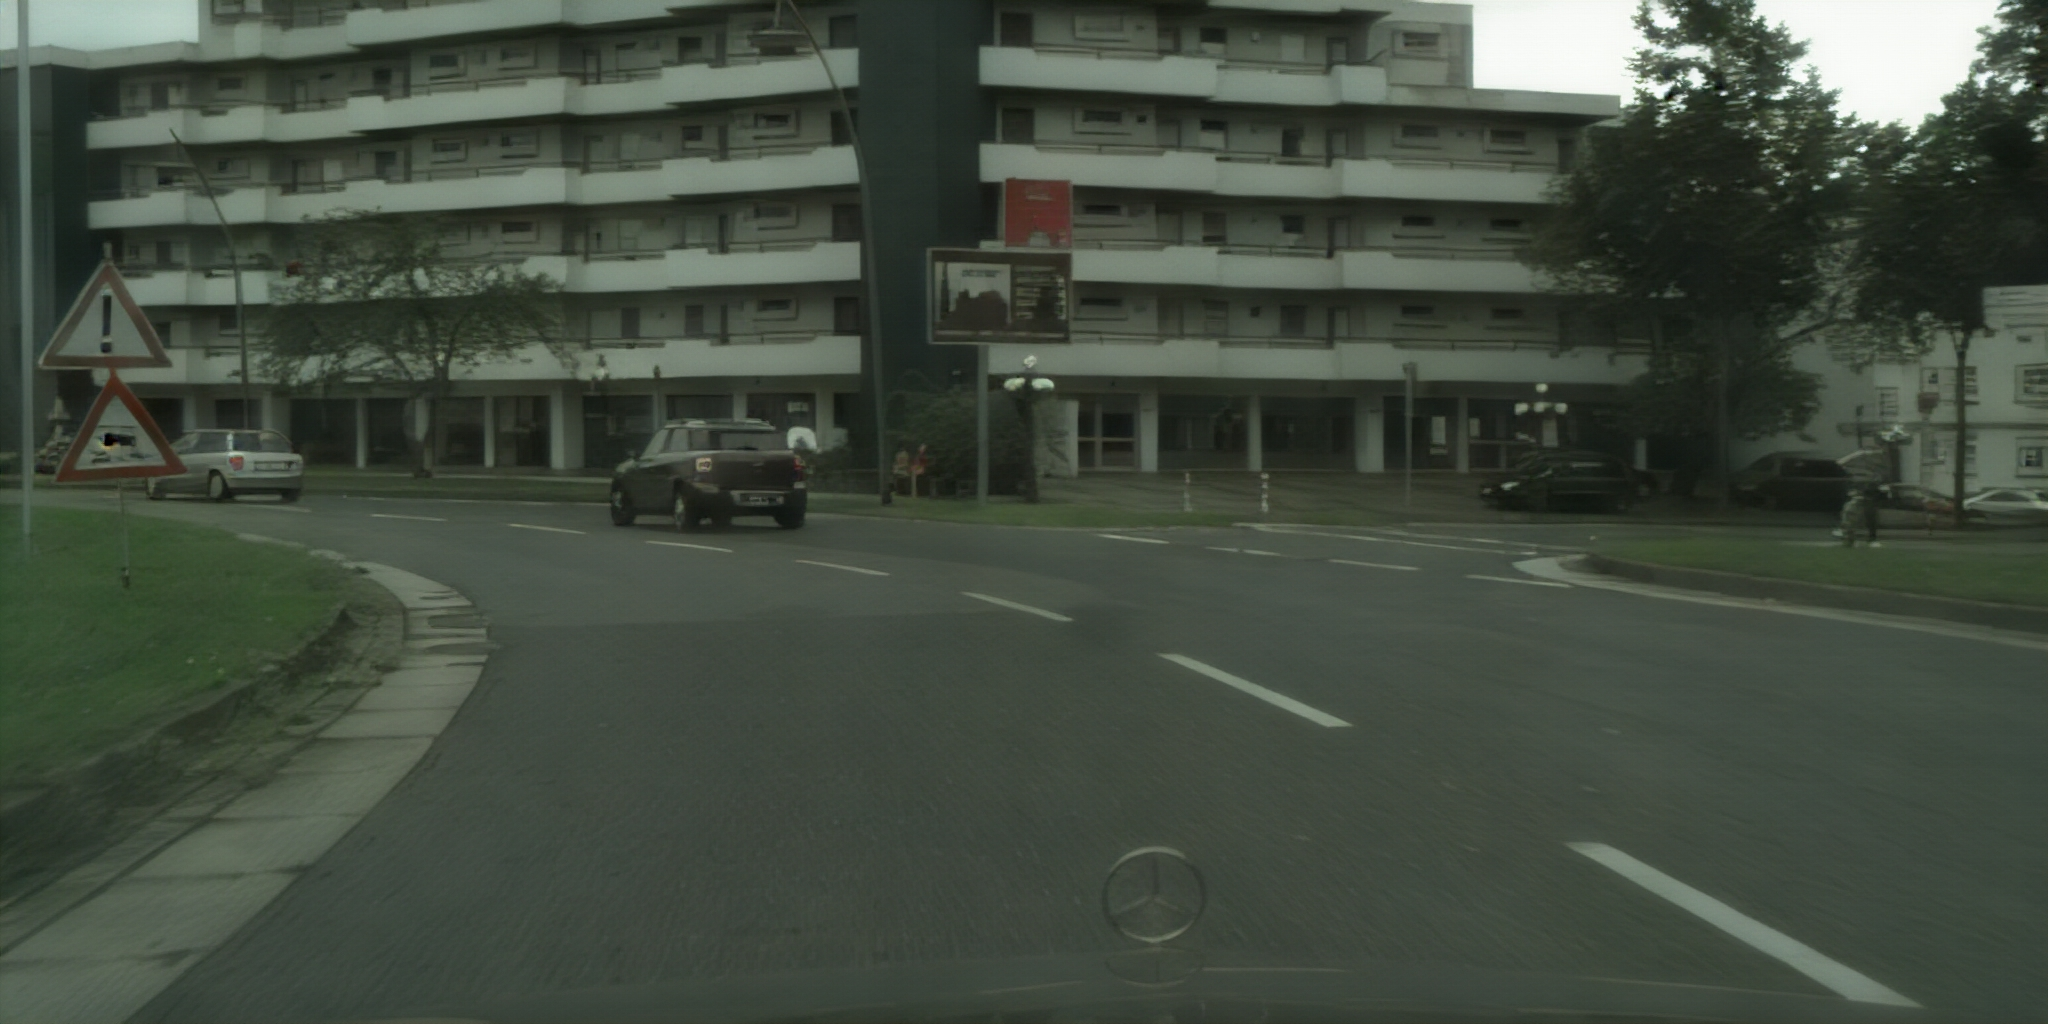
\includegraphics[scale=0.19]{pictures/img00_vq-f16.png}
                \caption{Rekonstruiertes Bild mit vq-f16 Modell (Aachen erstes Bild).}
                \label{fig:0_vq-f16_aachen_000000}
            \end{figure}

\newpage
            Original im Vergleich zum \textbf{vq-f8-n256} Modell      
            \begin{figure}[!htb]
                \centering
                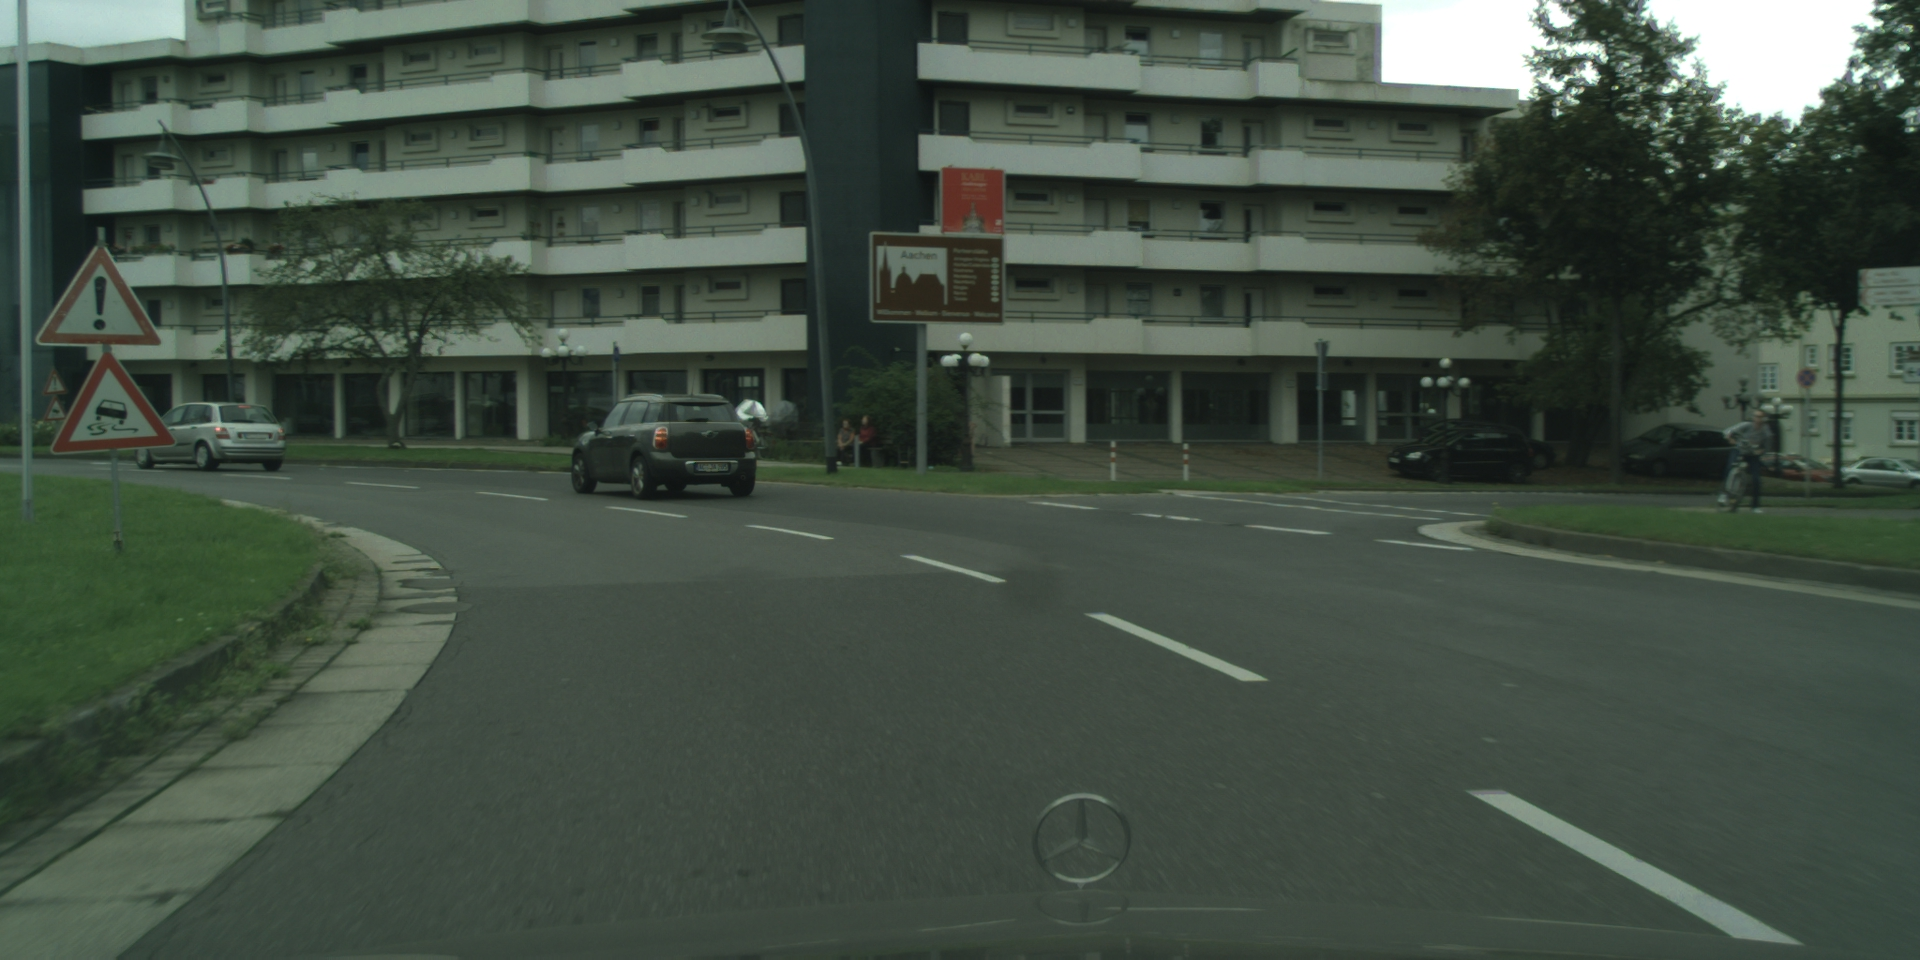
\includegraphics[scale=0.19]{pictures/img00_png.png}
                \caption{Originales Bild aus dem Cityscapes  Datensatz (Aachen erstes Bild).}
                \label{fig:og1_aachen_000000}
            \end{figure}
            \begin{figure}[!htb]
                \centering
                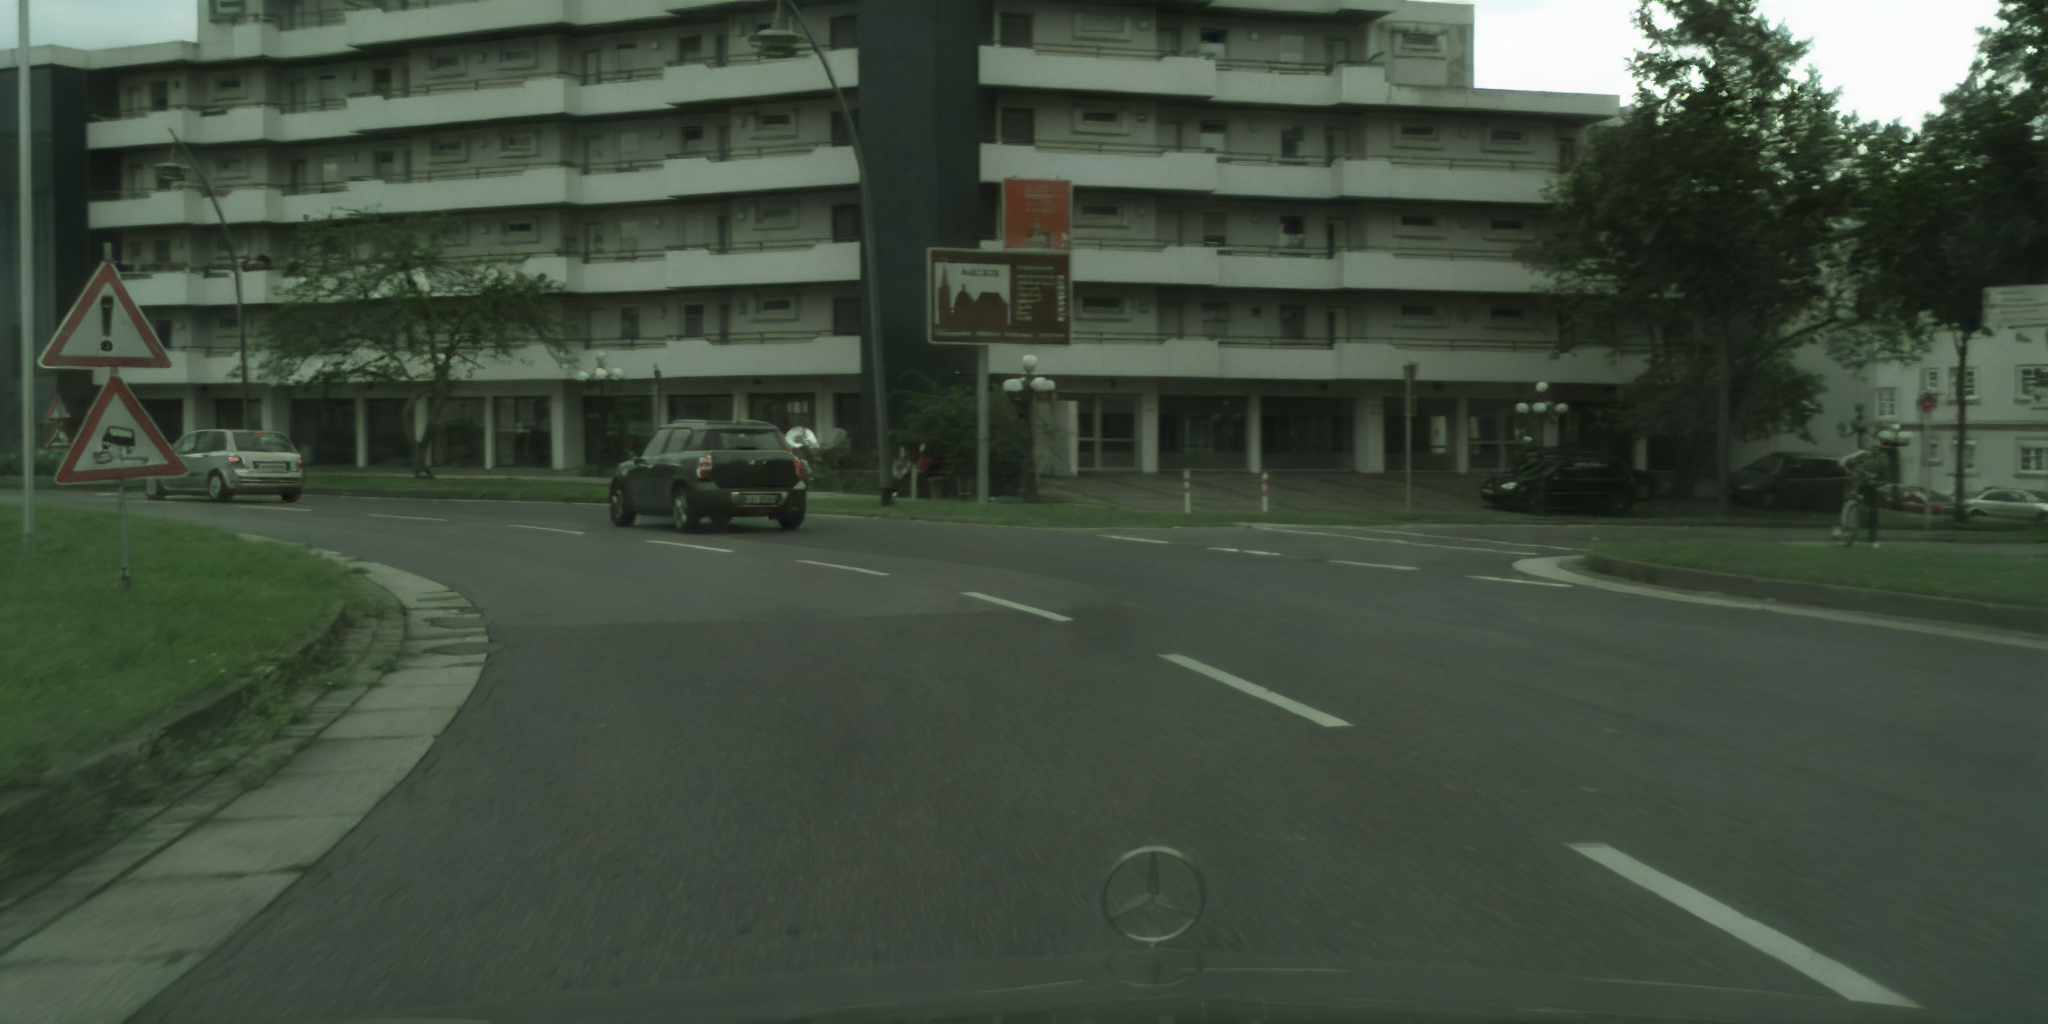
\includegraphics[scale=0.19]{pictures/img00_vq-f8-n256.png}
                \caption{Rekonstruiertes Bild mit vq-f8-n256 Modell (Aachen erstes Bild).}
                \label{fig:0_vq-f8-n256_aachen_000000}
            \end{figure}

\newpage
            \textbf{vq-f16} im Vergleich zu \textbf{vq-f8-n256} rekonstruierten Bild
\end{comment}
            \begin{figure}[!htb]
                \centering
                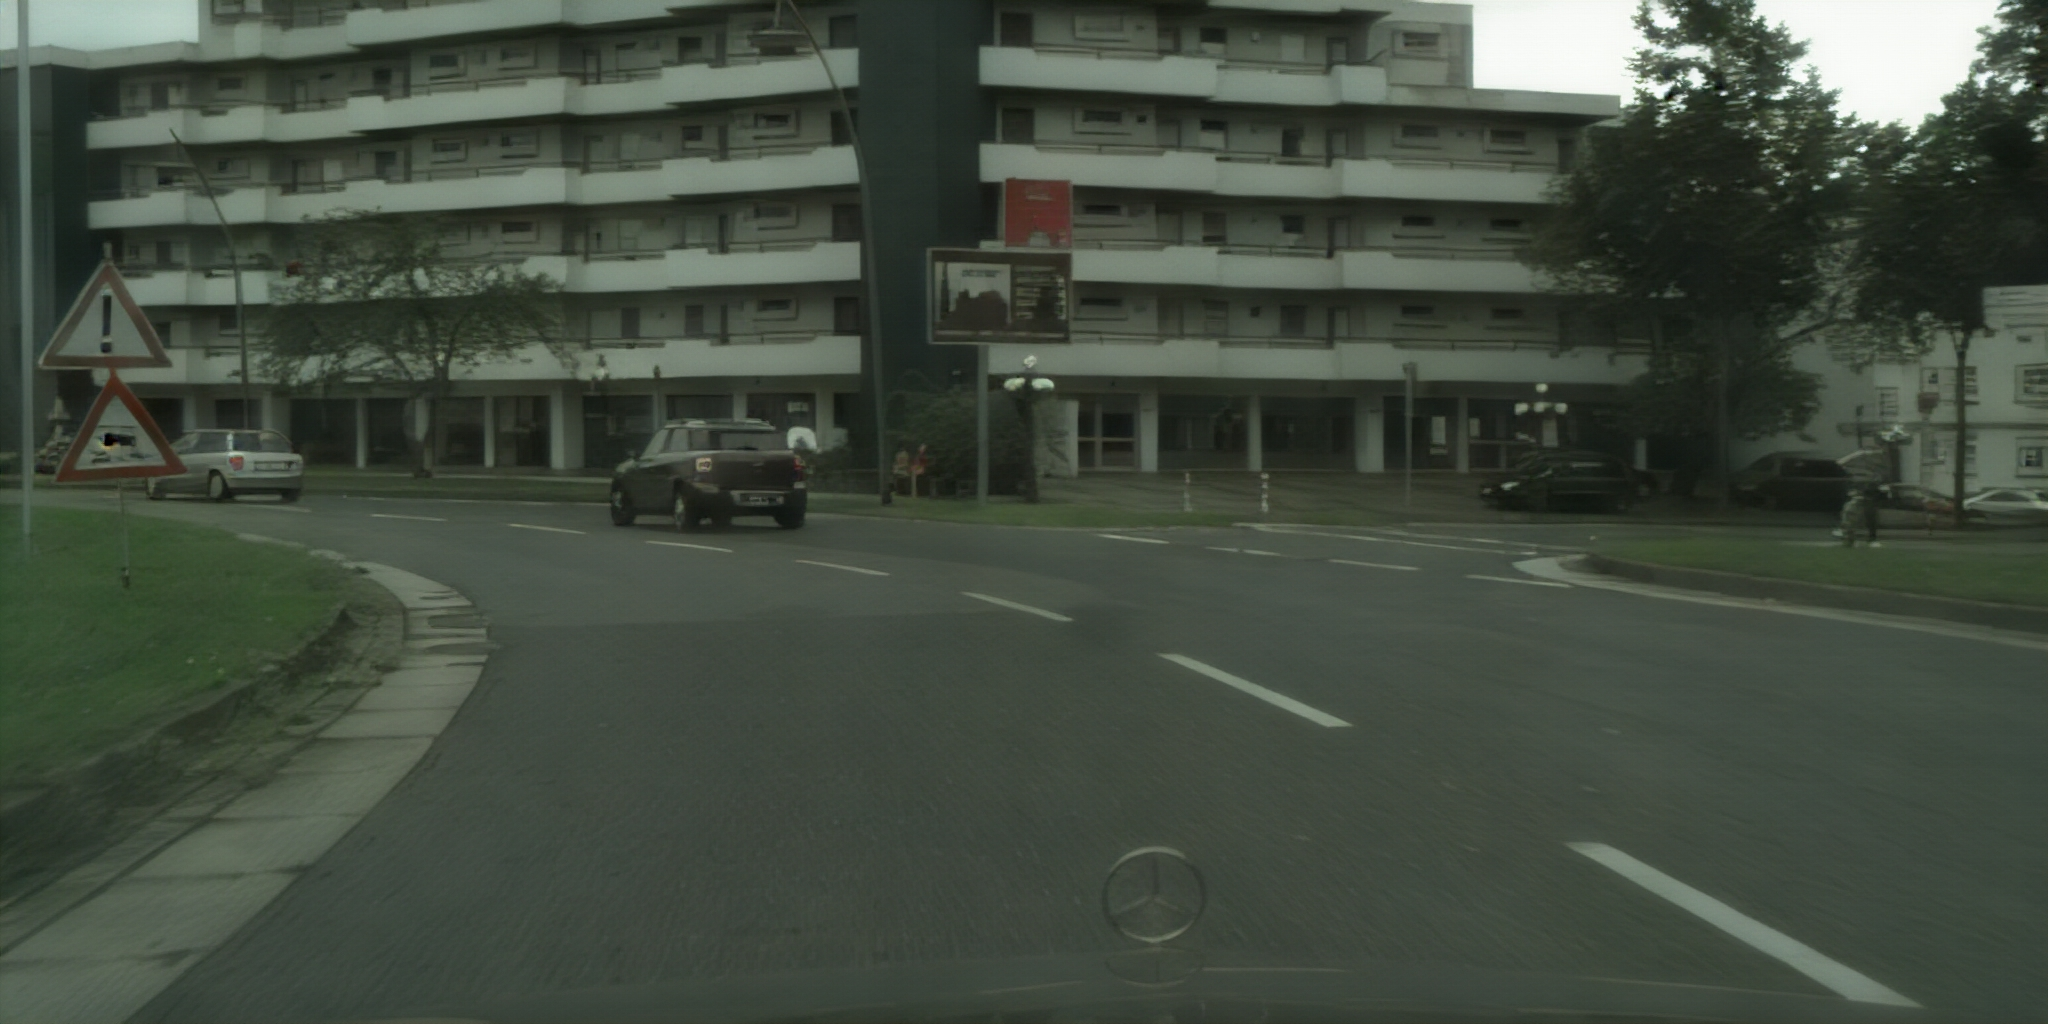
\includegraphics[scale=0.19]{pictures/img00_vq-f16.jpg}
                \caption{Rekonstruiertes Bild mit vq-f16 Modell (Aachen erstes Bild).}
                \label{fig:1_vq-f16_aachen_000000}
            \end{figure}
            \begin{figure}[!htb]
                \centering
                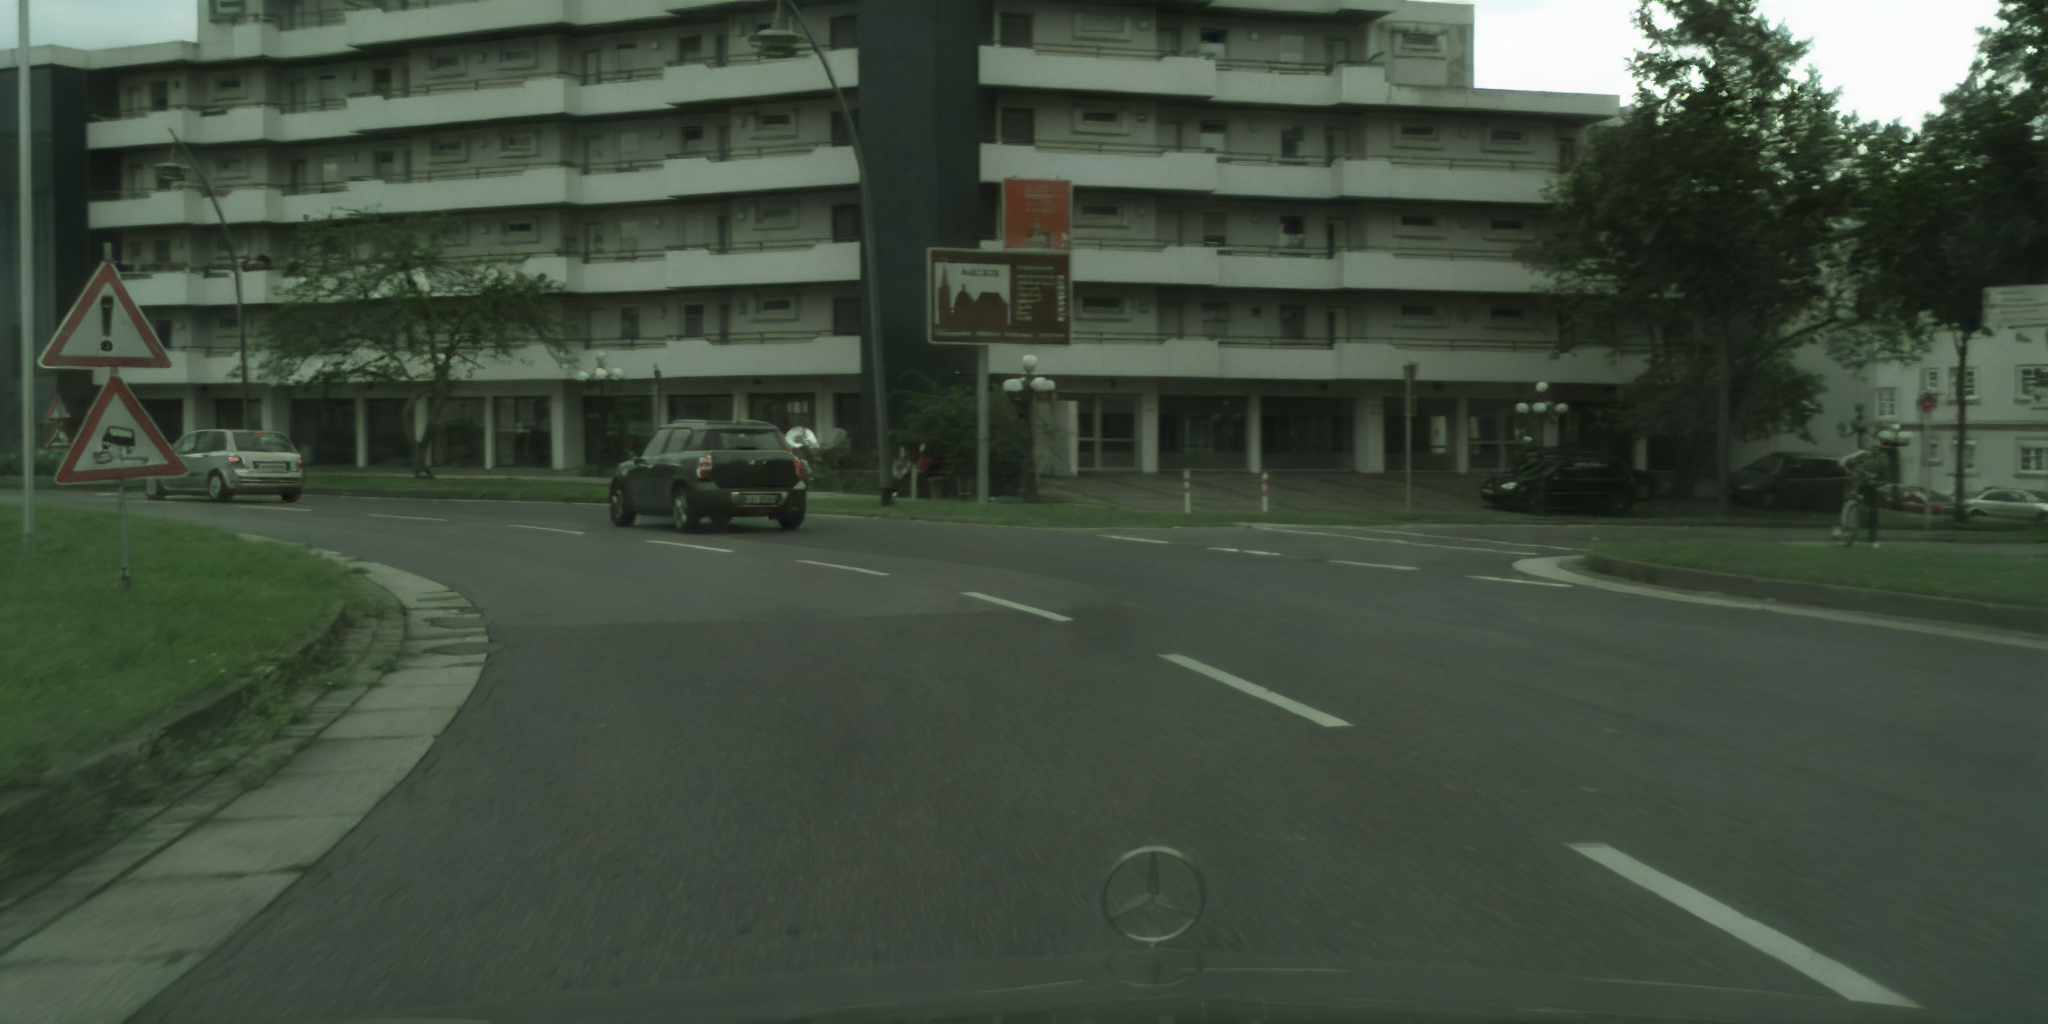
\includegraphics[scale=0.19]{pictures/img00_vq-f8-n256.jpg}
                \caption{Rekonstruiertes Bild mit vq-f8-n256 Modell (Aachen erstes Bild).}
                \label{fig:1_vq-f8-n256_aachen_000000}
            \end{figure}
            
\newpage  
            \begin{figure}[!htb]
                \centering
                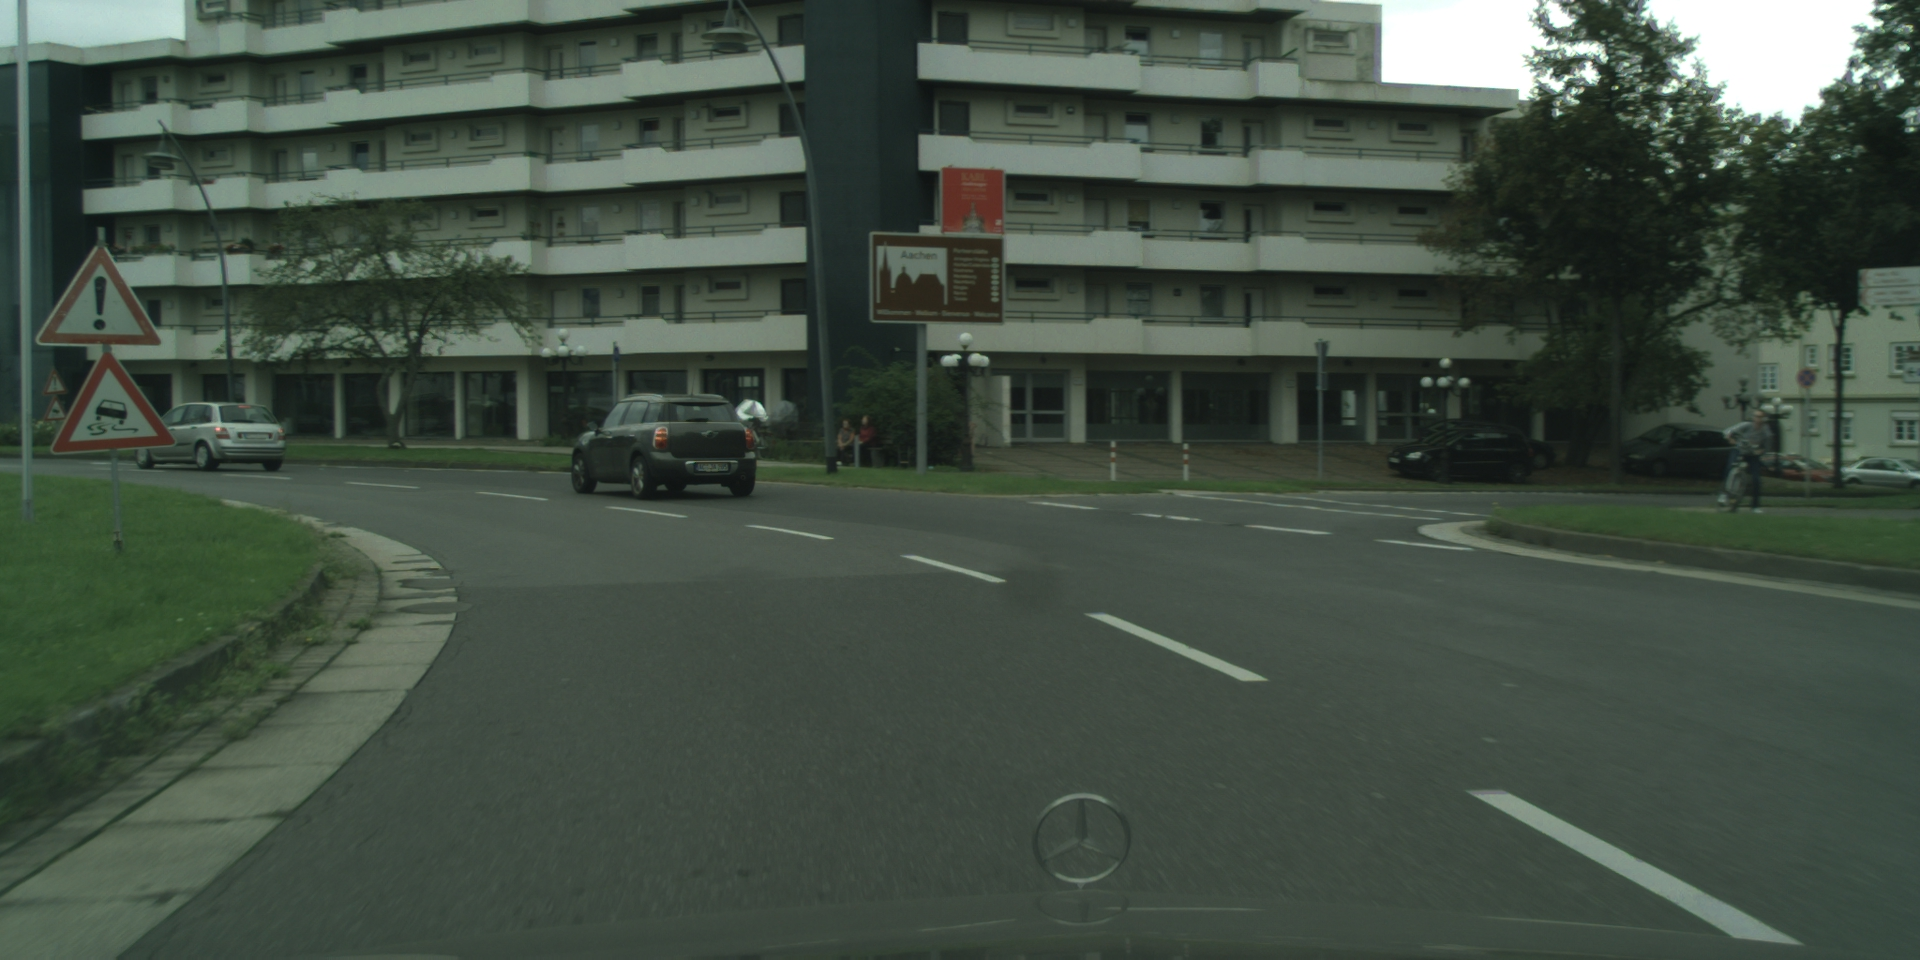
\includegraphics[scale=0.19]{pictures/img00_png.jpg}
                \caption{Originales Bild aus dem Cityscapes  Datensatz (Aachen erstes Bild).}
                \label{fig:og1_aachen_000000}
            \end{figure}
            Zwischen dem Originalbild und dem \textbf{vq-f16}-rekonstruierten Bild sind bei der Stärke der Kompression kaum oder nur geringe Veränderungen sichtbar.
            Dennoch sind Unterschiede in Farbe und Kontrast erkennbar. Auch Details wurden nicht mehr so präzise rekonstruiert. Das Nummernschild des Autos oder das Straßenschild zeigen eindeutig, dass das Bild nicht echt ist. Betrachtet man nun das Bild, welches das \textbf{vq-f8-n256}-Modell rekonstruiert hat, so ist es dem Original noch näher. Details, wie sie auf dem Schild zu erkennen sind, sind deutlich besser als bei dem Bild, welches das \textbf{vq-f16}-Modell erstellt hat. Obwohl der Kompressionsfaktor lediglich eine Differenz von $219,43 - 192 = 27,43$ aufweist, sind die Details der beiden modellbasiert rekonstruierten Bilder sehr unterschiedlich. Das Bild des \textbf{vq-f8-n256}-Modells ist für das menschliche Auge, was die Unterschiede zum Original betrifft, nur bei genauerer Betrachtung erkennbar. Selbst ein direkter Vergleich mit dem Original zeigt nicht auf Anhieb, dass es sich um zwei verschiedene Bilder handelt.

\newpage
            \begin{figure}[!htb]
                \centering
                \includesvg[scale=0.56]{graphs/output_plot_mse_model.svg}
                \caption{MSE in Abhängigkeit zum Kompressionsfaktor. Vergleich zwischen JPEG-Kompression und KI-Modell rekonstruierter Bilder.}
                \label{fig:output_plot_mse_model}
            \end{figure}

            Es zeigt sich, dass der MSE des \textbf{vq-f16} ähnlich hoch ist wie der des JPEG-Datensatzes mit einer Kompressionsqualität von $5\%$, obwohl bei direktem Vergleich der Bilder mit bloßem Auge sofort erkennbar ist, dass ein deutlicher qualitativer Unterschied besteht.\\          
            
            \begin{figure}[!htb]
                \centering
                \begin{minipage}[!htb]{0.47\textwidth}
                    \centering
                    \textbf{Komprimiert ($5\%$)} % Überschrift für die erste Spalte
                \end{minipage}
                %
                \begin{minipage}[!htb]{0.47\textwidth}
                    \centering
                    \textbf{\textbf{vq-f16}} % Überschrift für die zweite Spalte
                \end{minipage}

                \begin{minipage}[!htb]{0.47\textwidth}
                    \centering
                    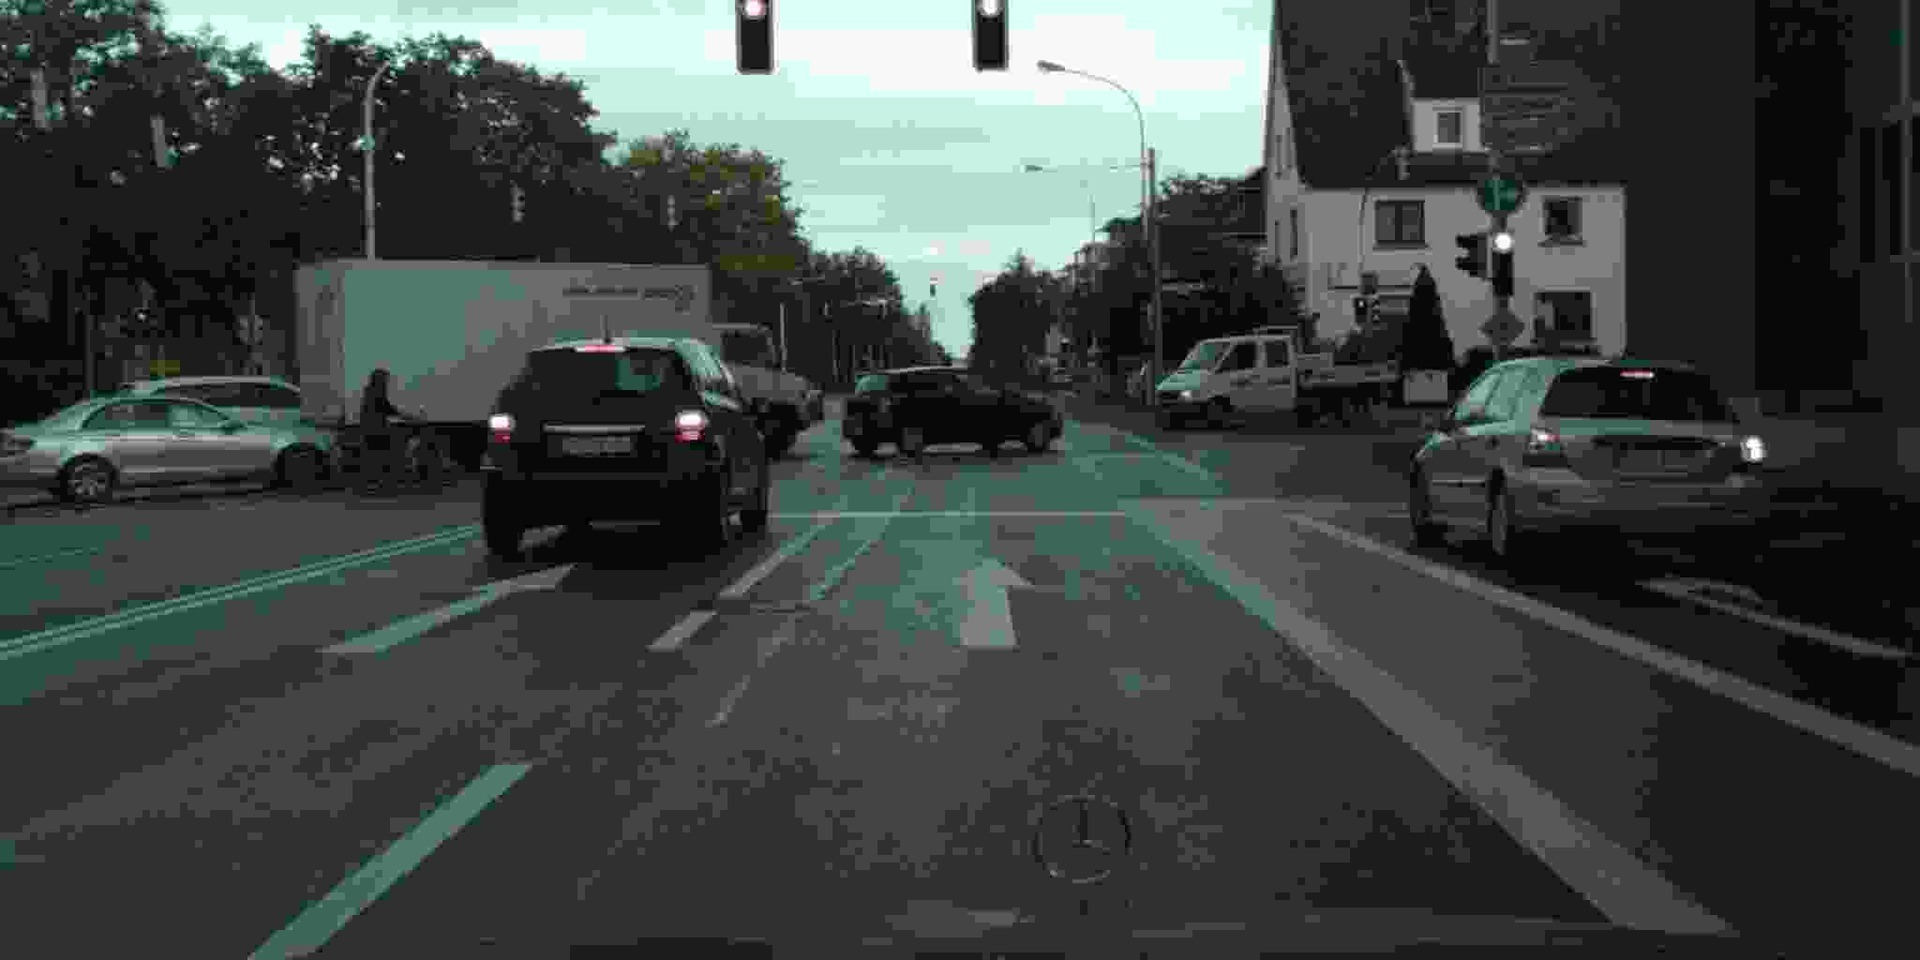
\includegraphics[width=\textwidth]{pictures/img_jpg5_darmstadt_000002.jpg}    
                    \label{fig:bild132}
                \end{minipage}
                %
                \begin{minipage}[!htb]{0.47\textwidth}
                    \centering
                    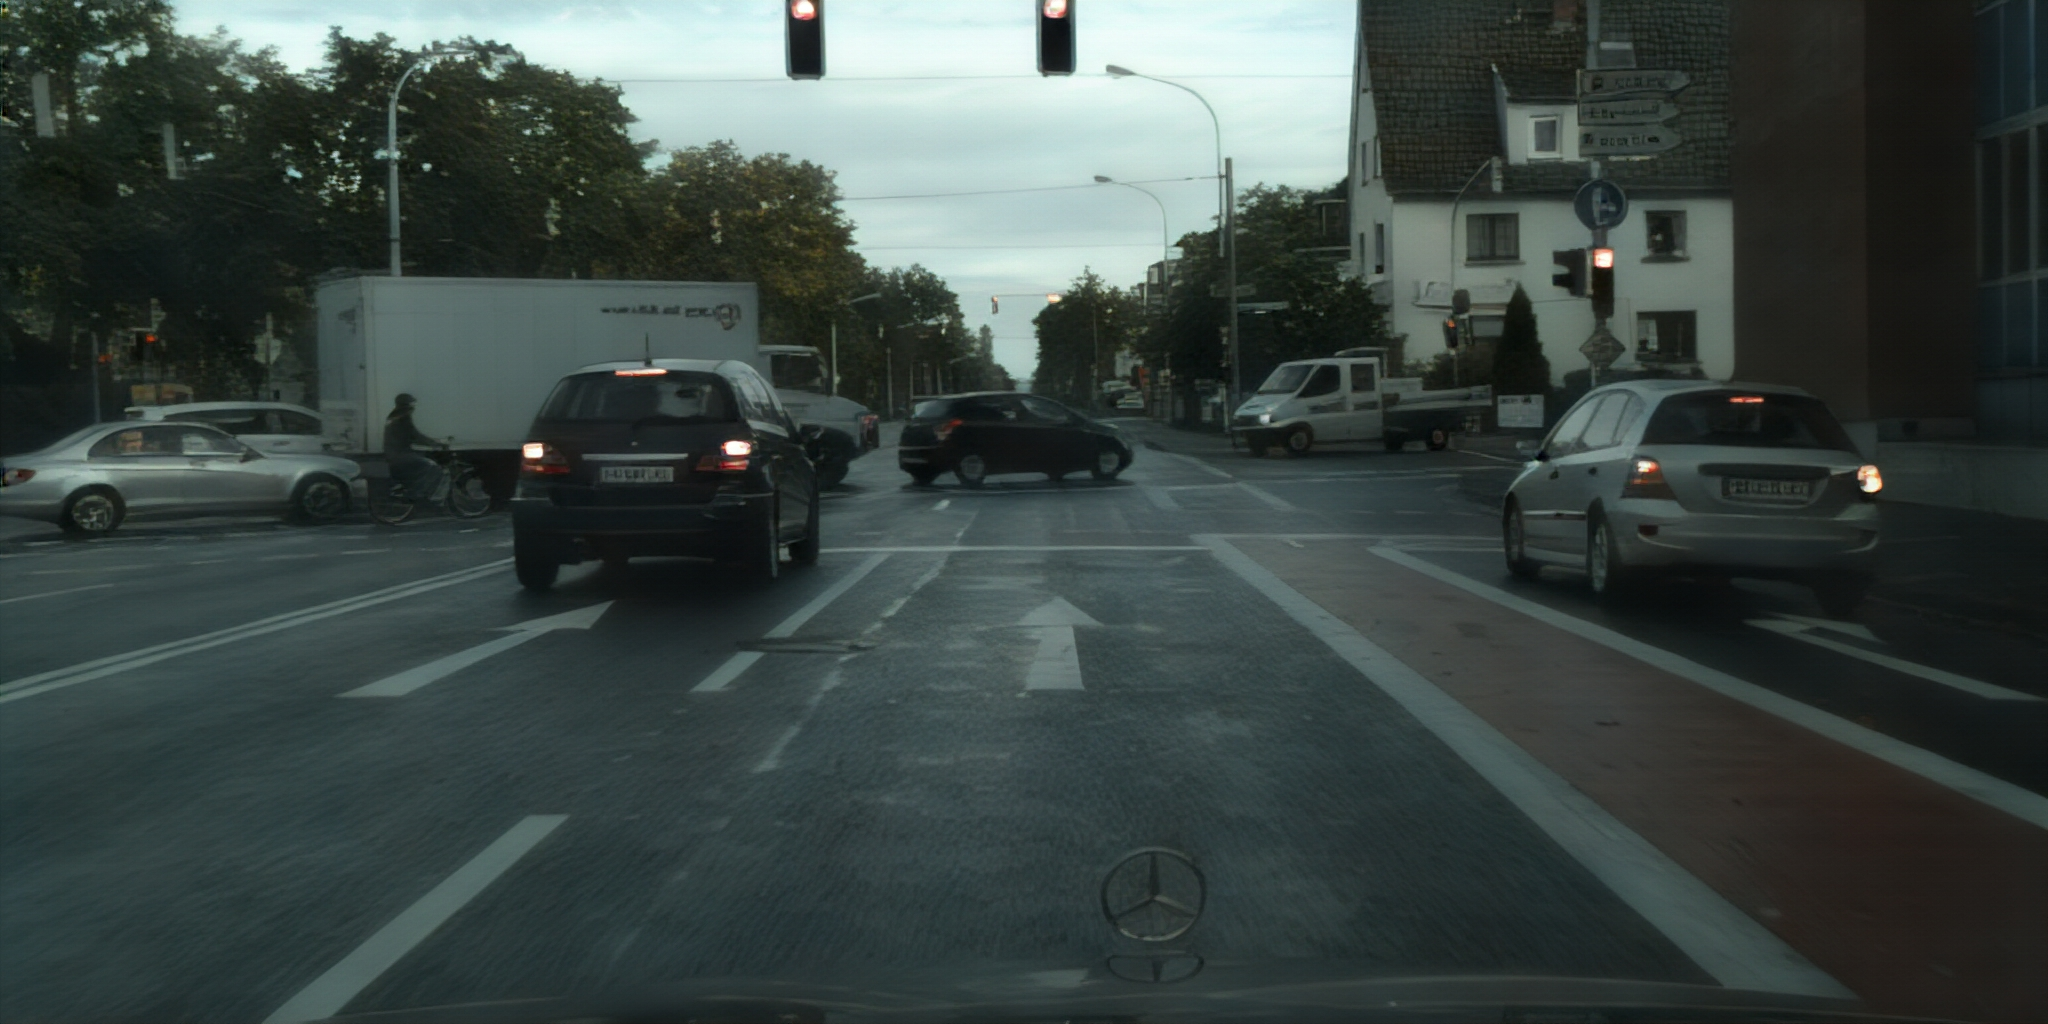
\includegraphics[width=\textwidth]{pictures/vq-f16_darmstadt_000002.jpg}
                    \label{fig:bild142}
                \end{minipage}
            \end{figure}

            Dies zeigt, dass der MSE nicht besonders gut geeignet ist, um die Qualität eines Bildes zu bestimmen. MSE sowie PSNR berücksichtigen nicht die menschliche Wahrnehmung des Auges, wie es der SSIM tut, was die Bewertung eines Bildes betrifft \cite{mse_psnr_eye}.
\newpage
            \begin{figure}[!htb]
                \centering
                \begin{minipage}[!htb]{0.47\textwidth}
                    \centering
                    \textbf{Komprimiert ($10\%$)} % Überschrift für die erste Spalte
                \end{minipage}
                %
                \begin{minipage}[!htb]{0.47\textwidth}
                    \centering
                    \textbf{\textbf{vq-f8-n256}} % Überschrift für die zweite Spalte
                \end{minipage}

                \begin{minipage}[!htb]{0.47\textwidth}
                    \centering
                    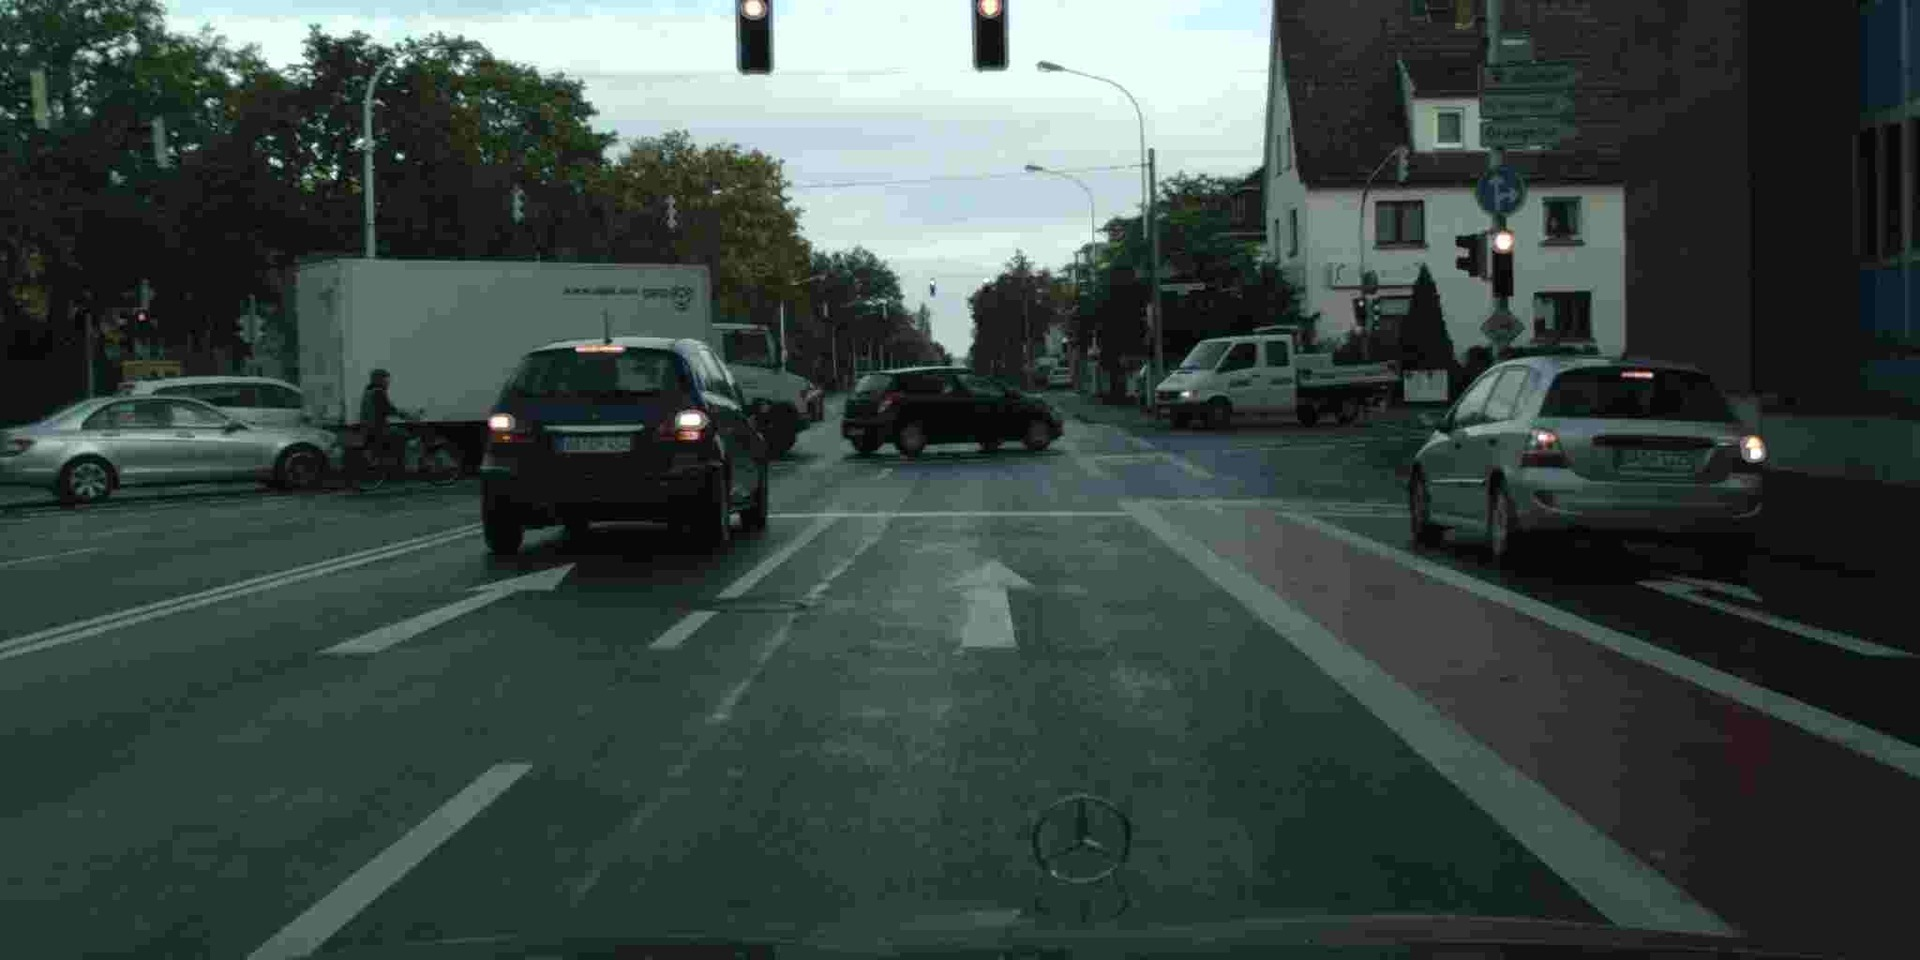
\includegraphics[width=\textwidth]{pictures/jpg10_darmstadt_000002.jpg}    
                \end{minipage}
                %
                \begin{minipage}[!htb]{0.47\textwidth}
                    \centering
                    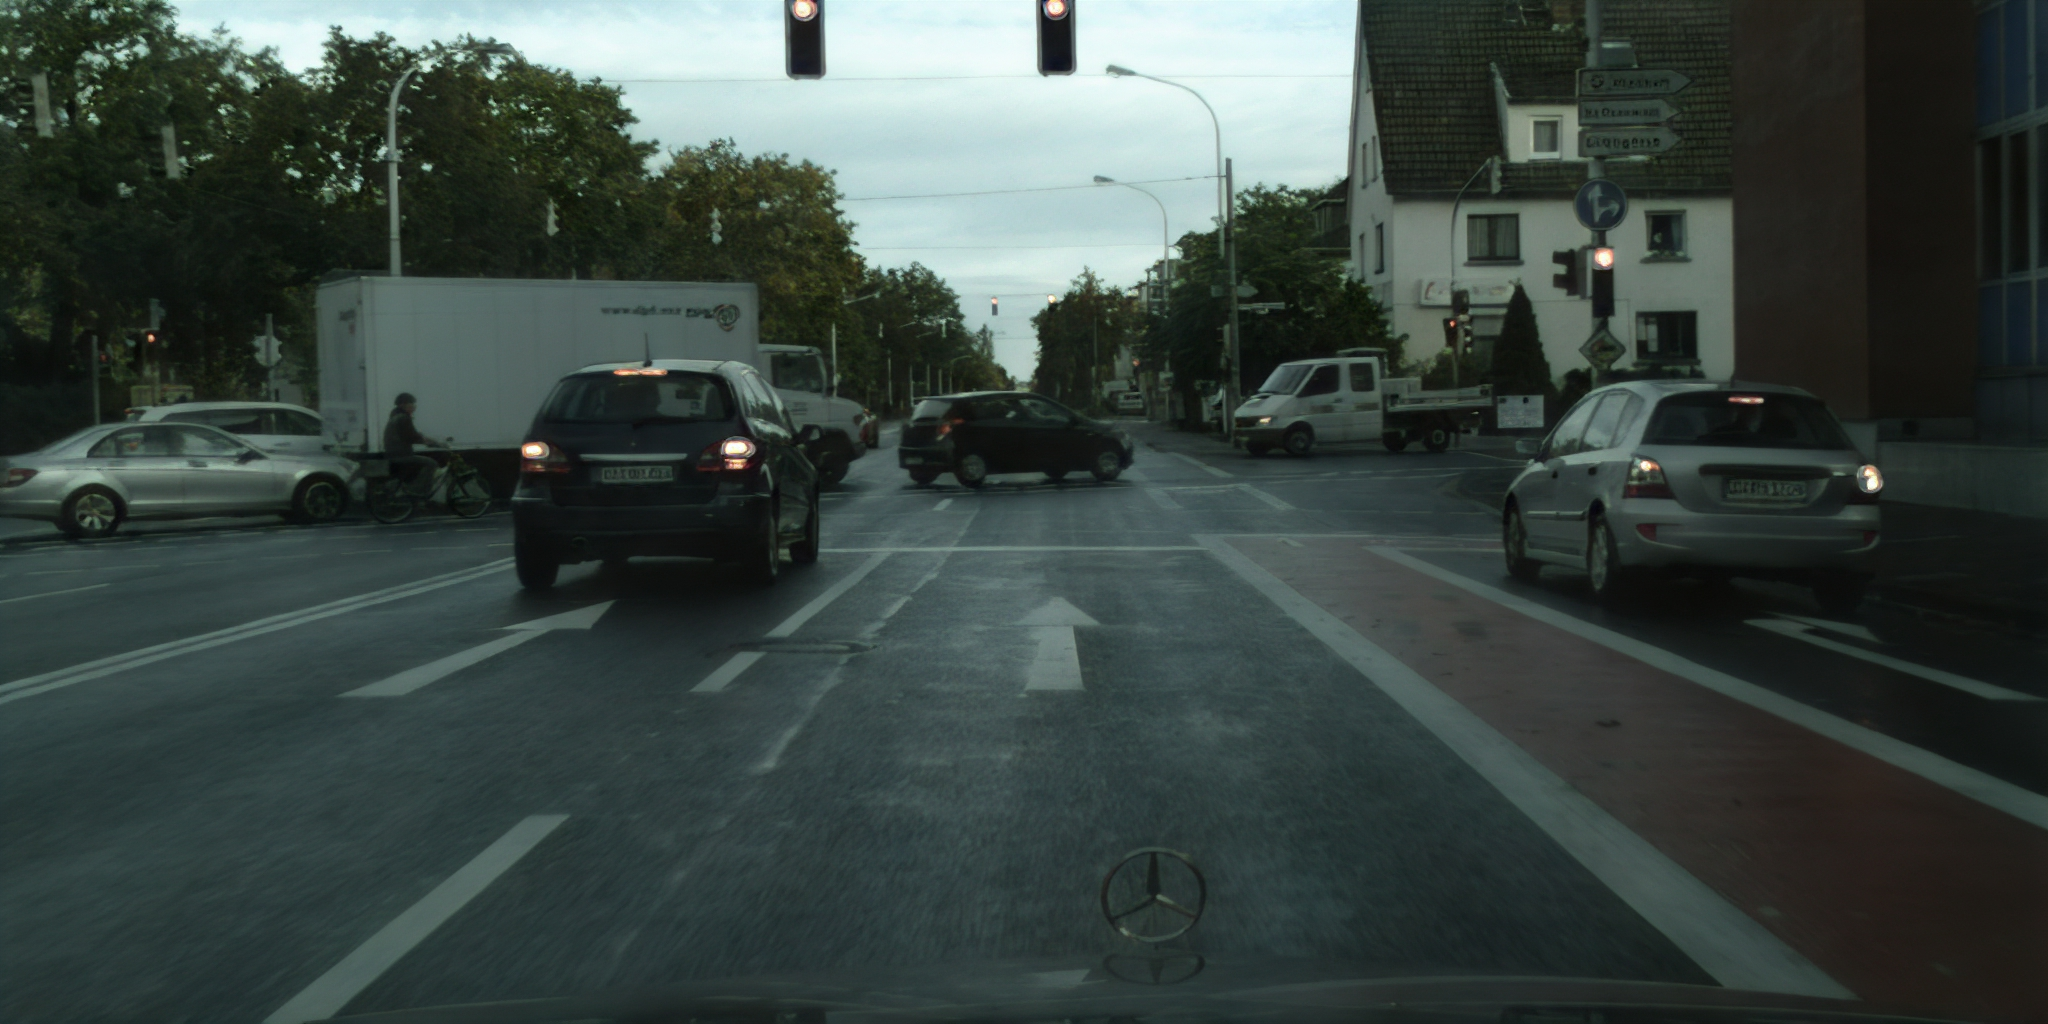
\includegraphics[width=\textwidth]{pictures/vq-f8-n256_darmstadt_000002.jpg}
                \end{minipage}
            \end{figure}

            Auch der MSE des \textbf{vq-f8-n256} ist mit $9,8e^{-4}$ hoch und größer als der der Bilder mit einer Kompressionsqualität von $10\%$ mit $8,07e^{-4}$. Der MSE ist somit kein Maßstab, mit dem sich Bilder gut auf ihre Qualität überprüfen lassen. Auch hier zeigt sich das, obwohl der MSE des \textbf{vq-f8-n256}-Modells schlechter ist, die Bilder jedoch qualitativ hochwertiger sind.

            \begin{figure}[!htb]
                \centering
                \includesvg[scale=0.56]{graphs/output_plot_psnr_model.svg}
                \caption{PSNR in Abhängigkeit zum Kompressionsfaktor. Vergleich zwischen JPEG-Kompression und KI-Modell rekonstruierter Bilder.}
                \label{fig:output_plot_psnr_model}
            \end{figure}

            Auch beim PSNR zeigen beide Modelle schlechte Ergebnisse, mit PSNR-Werten von $76,52$ für das \textbf{vq-f16}-Modell und $78,46$ für das \textbf{vq-f8-n256}-Modell. Auch hier liegen, wie bereits beim MSE, beide Modelle mit ihren Werten in Bezug auf die Qualität zwischen den JPEG-Datensätzen mit einer Kompressionsqualität von $5\%$ und $10\%$. Dies steht jedoch im Widerspruch zur Qualitätswahrnehmung des menschlichen Auges, wie im direkten Vergleich der Bilder sichtbar wird.
\newpage
            \begin{figure}[!htb]
                \centering
                \includesvg[scale=0.56]{graphs/output_plot_ssim_model.svg}
                \caption{SSIM in Abhängigkeit zum Kompressionsfaktor. Vergleich zwischen JPEG-Kompression und KI-Modell rekonstruierter Bilder.}
                \label{fig:output_plot_ssim_model}
            \end{figure}

            In der obigen Grafik werden die Datensätze der traditionellen Kompression und der beiden Modelle im Vergleich zum SSIM gegenübergestellt. Es ist direkt erkennbar, dass die beiden Modelle deutlich besser abschneiden als bei MSE und PSNR. Beim SSIM liegen die beiden Modelle nicht zwischen den Datensätzen mit $5\%$ und $10\%$ Kompressionsqualität, was einem Wertebereich von $63,45 - 80,07$ entsprechen würde. Das \textbf{vq-f16}-Modell erzielt einen SSIM-Wert von $87,69$, während das \textbf{vq-f8-n256}-Modell mit einem Wert von $90,2$ abschneidet. Das \textbf{vq-f8-n256}-Modell erreicht somit sogar einen Wert, der zwischen den Datensätzen der Kompressionsqualität von $15\%$ und $20\%$ liegt.
            Dies zeigt, dass der SSIM für die Beschreibung der Bildqualität eindeutig besser geeignet ist, da er Helligkeit, Kontrast und Struktur berücksichtigt.
            
            Die Qualitätsdifferenz der beiden Modelle untereinander ist bei SSIM und PSNR geringer mit $3\%$ Unterschied, bei MSE weisen die beiden Modelle eine Differenz von $37\%$ auf.
            Die beiden Modelle schneiden im Vergleich zueinander ähnlich ab bei SSIM sowie bei PSNR, bei MSE 
            gibt es zwischen den Modellen jedoch eine große Lücke.
            
\newpage
    \section{Performance der Objektdetektion}
        Die einzelnen Datensätze sind hinsichtlich ihrer Kompression und Qualität durch Metriken wie SSIM, PSNR und MSE untersucht. Der nächste Schritt dieser Arbeit besteht darin, die einzelnen Datensätze in ein KI-Modell zu überführen. \\
        Ziel ist es, Boundingboxen um Objekte zu erzeugen und die Auswirkungen unterschiedlicher Kompressionsqualitäten sowie Kompressionsfaktoren auf die Objektdetektion zu messen. Der Originaldatensatz wird ebenfalls mit Boundingboxen versehen und dient als Referenz, wobei die Ground-Truth-Boundingboxen als Label verwendet werden.
        Dies ist notwendig, da die Boundingboxen des Cityscapes-Datensatzes mit einem anderen Modell erstellt wurden. Es werden jedoch die gleichen Grundvoraussetzungen benötigt, d.h. die Labels und die Datensätze, die für die Objekterkennung verwendet werden, müssen mit demselben Modell erstellt worden sein für gleiche Bedingungen, um miteinander verglichen werden zu können.
    
        Als Modell wurde ein vortrainiertes Netz von Ultralytics YOLO verwendet. Das YOLO-Modell (You Only Look Once), ein bedeutender Ansatz für Objekterkennung und Bildsegmentierung, wurde von Joseph Redmon und Ali Farhadi an der University of Washington entwickelt. Seit seiner Einführung im Jahr 2015 hat YOLO durch seine herausragende Kombination aus Geschwindigkeit und Präzision schnell an Popularität gewonnen.
        Das YOLO11-Modell, welches im Rahmen dieser Untersuchung verwendet wurde, ist zum Stand dieser Arbeit das neueste und State-of-the-Art-Modell von YOLO. Es wurde auf dem COCO-Datensatz trainiert und ist laut Angaben der Entwickler für Objekterkennung, Instanzsegmentierung, Bildklassifikation, Pose-Schätzung und die Erkennung orientierter Objekte (OBB) geeignet \cite{yolo_modell}.

        Der Originaldatensatz wurde mithilfe des Modells verarbeitet, und es wurden Boundingboxen um erkannte Objekte gelegt. Dieser neue Datensatz, der dadurch entstand, dient als Ground-Truth-Label-Datensatz für die weiteren Untersuchungen (siehe Kapitel 4, Konzept).

\newpage
        Zwei Label Bilder, welche das YOLO-Modell erzeugt hat, aus dem Originaldatensatz.
        Zu erkennen sind die Ground-Truth-Boundingboxen, farblich gekennzeichnet, abhängig von der Klasse.
        Die Zahl gibt den prozentualen Wert an, wie sicher sich das Modell dabei ist. Dieser spielt aber keine Rolle, da es sich hier um die generierten Ground-Truth-Boundingboxen handelt.
    
        \begin{figure}[!htb]
            \centering
            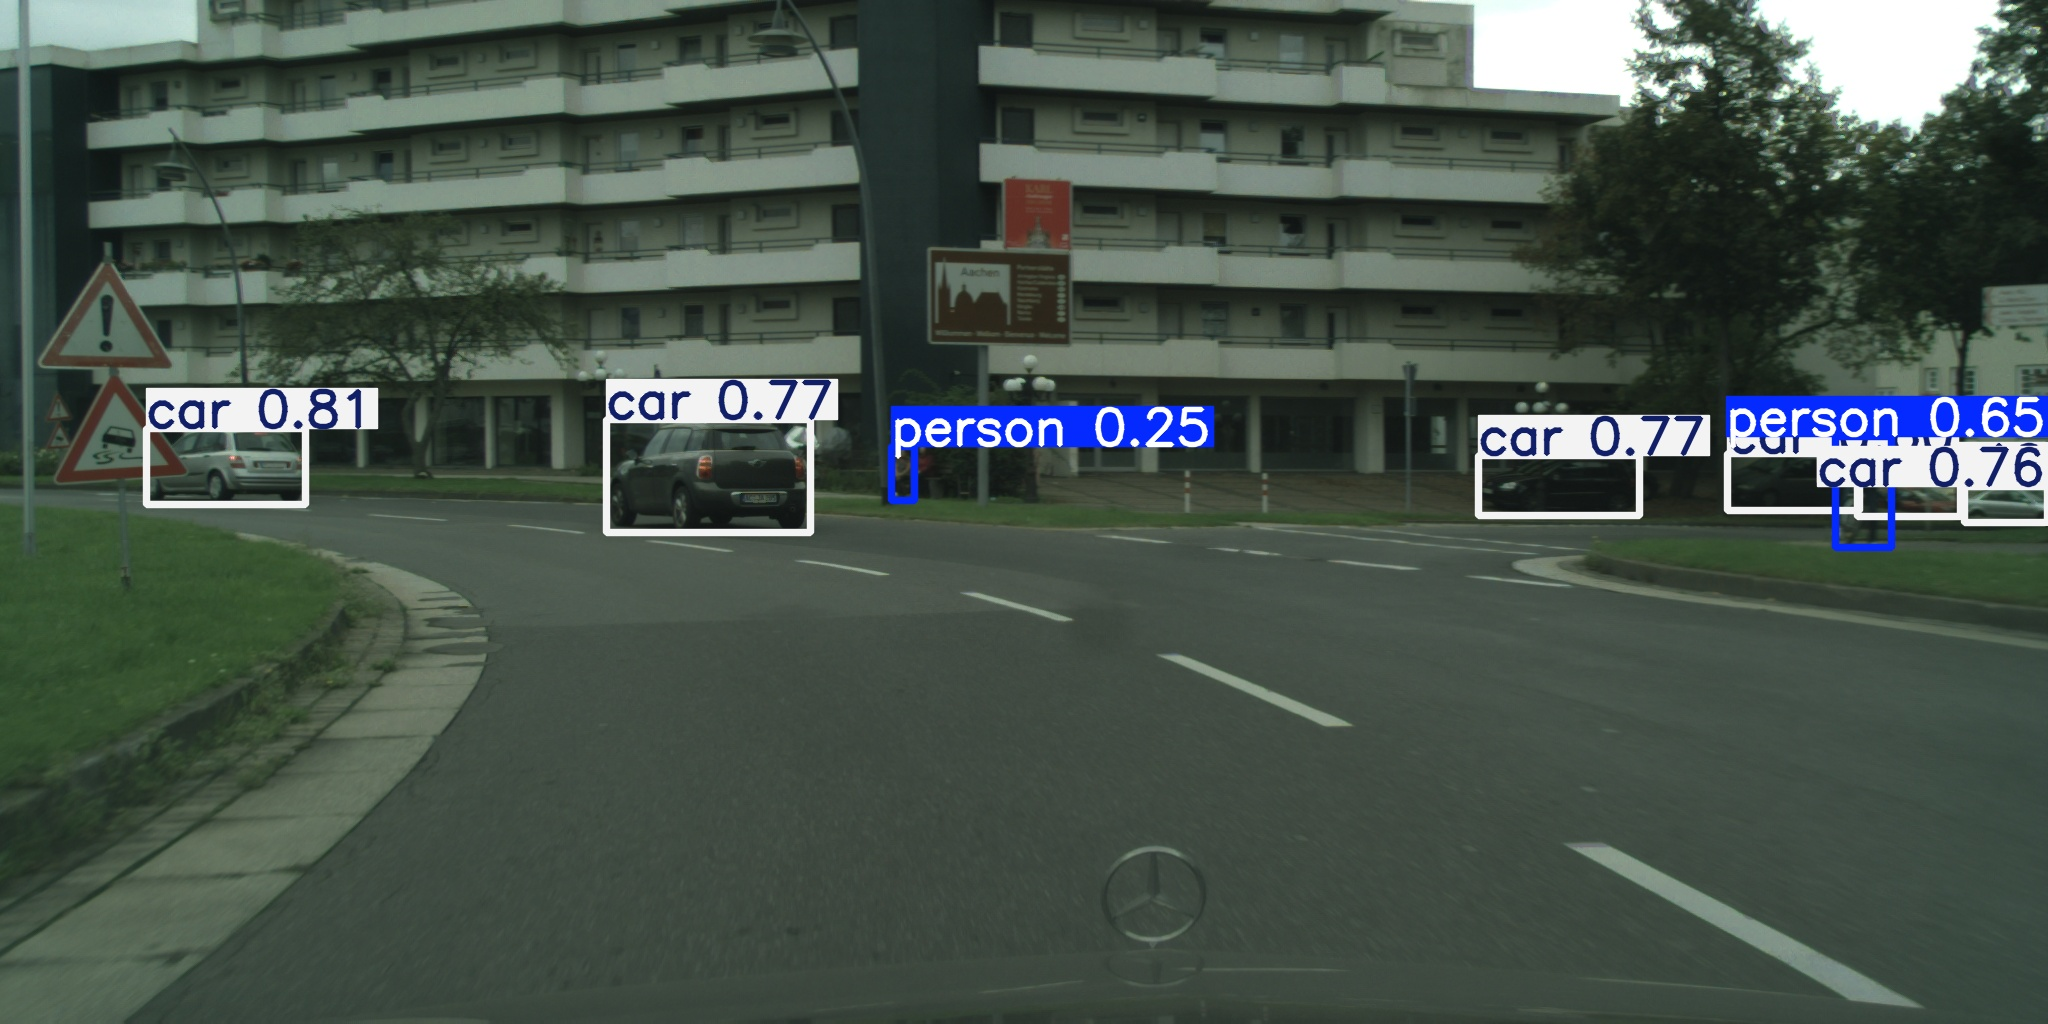
\includegraphics[scale=0.19]{pictures/original_aachen_000000.jpg}
            \caption{Erzeugtes Label aus dem Original Cityscapes Datensatz (Aachen erstes Bild) zur Objekterkennung durch das YOLO-Model.}
            \label{fig:og_aachen_000000}
        \end{figure}
        \begin{figure}[!htb]
            \centering
            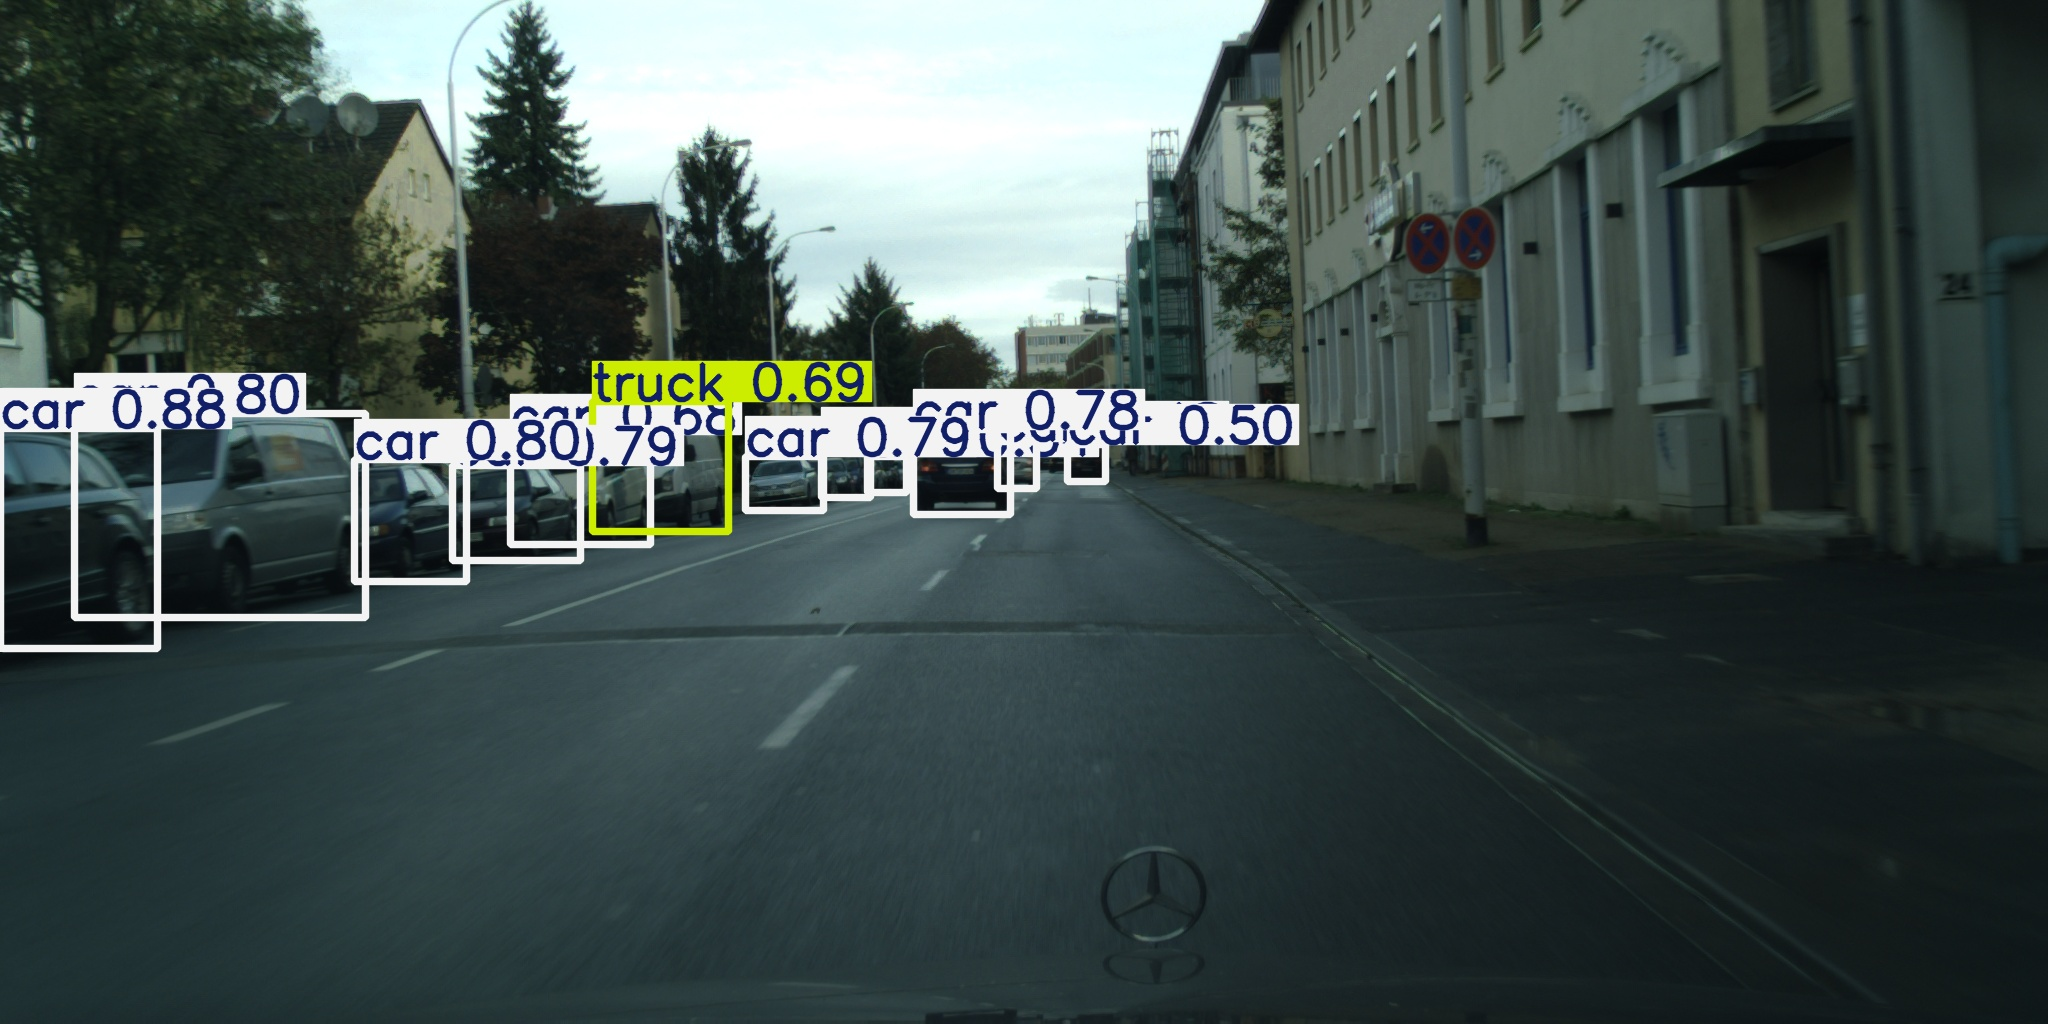
\includegraphics[scale=0.19]{pictures/original_darmstadt_000000.jpg}
            \caption{Erzeugtes Label aus dem Original Cityscapes Datensatz (Darmstadt drittes Bild) zur Objekterkennung durch das YOLO-Model.}
            \label{fig:og_darmstadt_000000}
        \end{figure}

\newpage  
        \subsection{JPEG-komprimierte Bilder}
            Für jedes Bild in den JPEG-Datensatz wurden Boundingboxen erstellt.
            \begin{figure}[!htb]
                \centering
                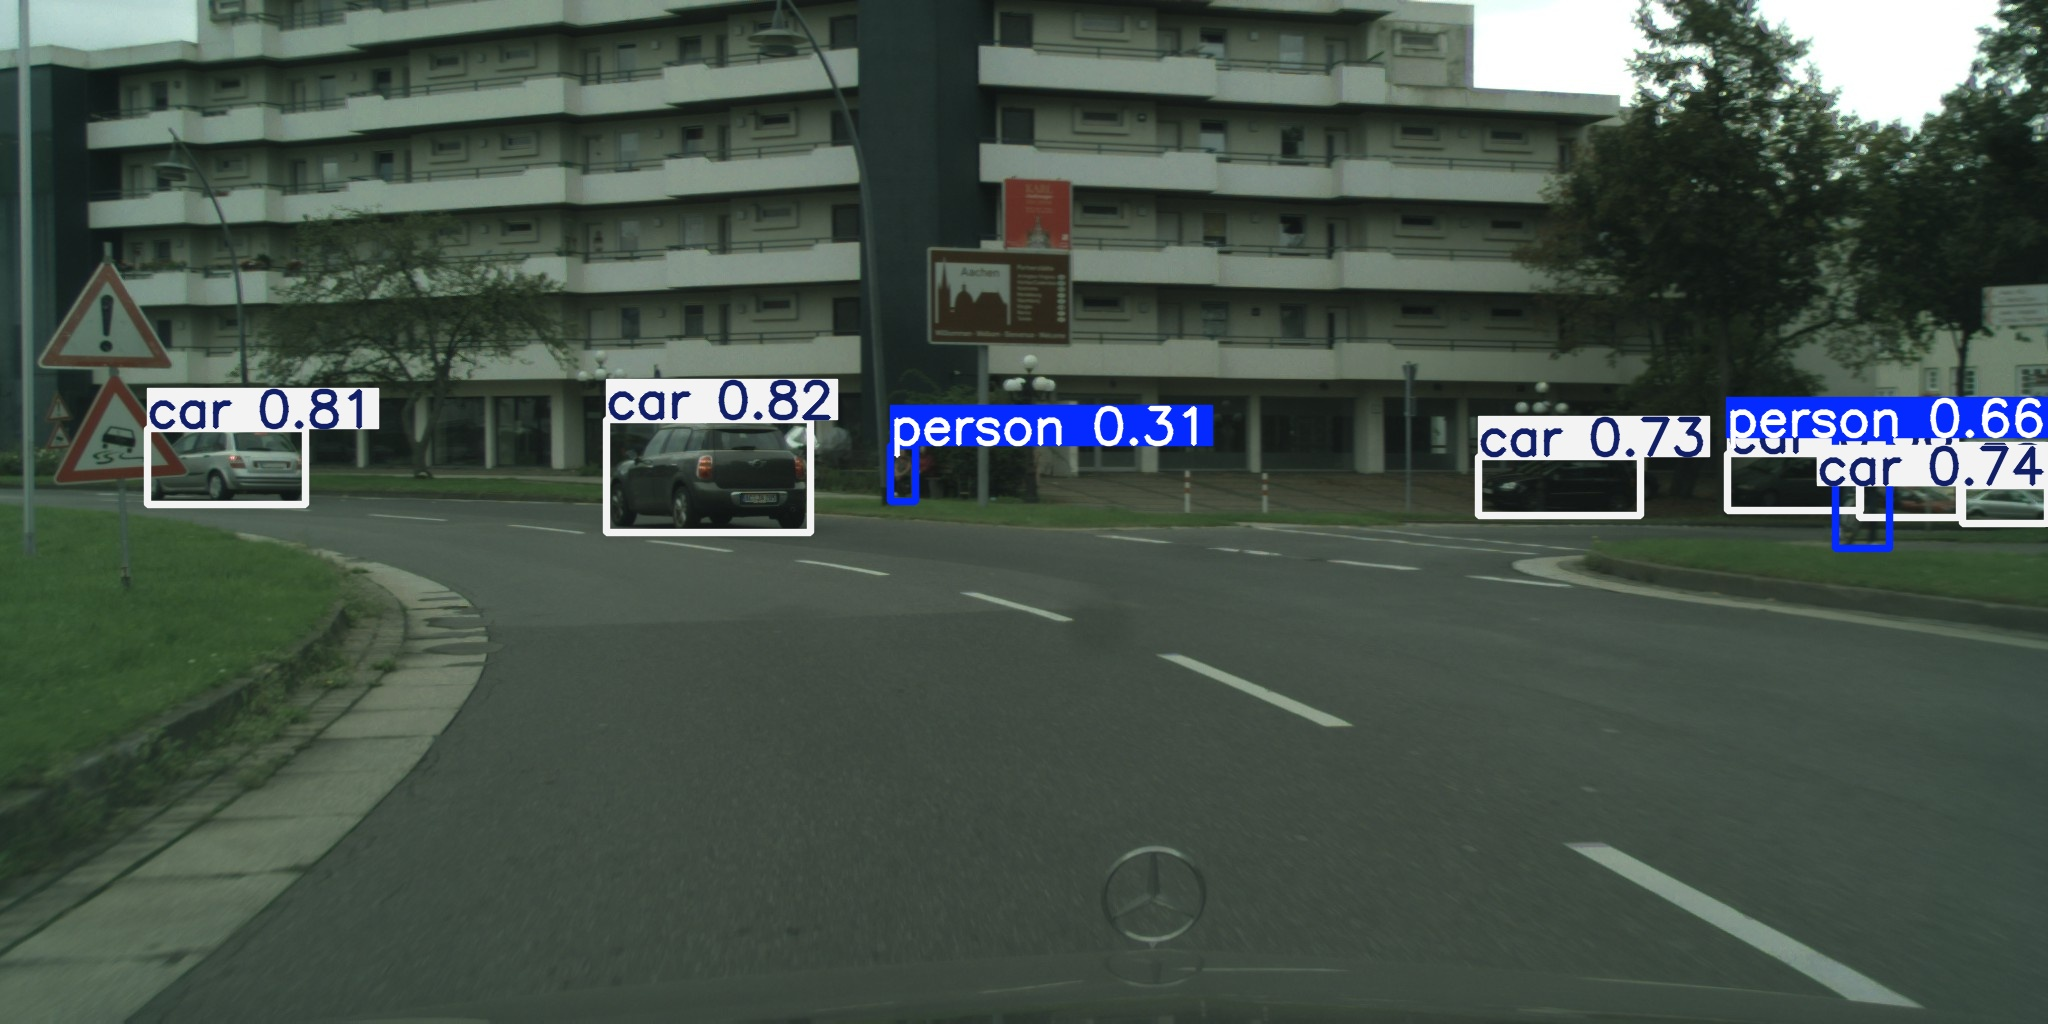
\includegraphics[scale=0.19]{pictures/jpg90_aachen_000000.jpg}
                \caption{Bild mit einer Kompressionsqualität von $90\%$ (Aachen, erstes Bild) zur Objekterkennung mit dem YOLO-Modell.}
                \label{fig:90_aachen_000000}
            \end{figure}
            \begin{figure}[!htb]
                \centering
                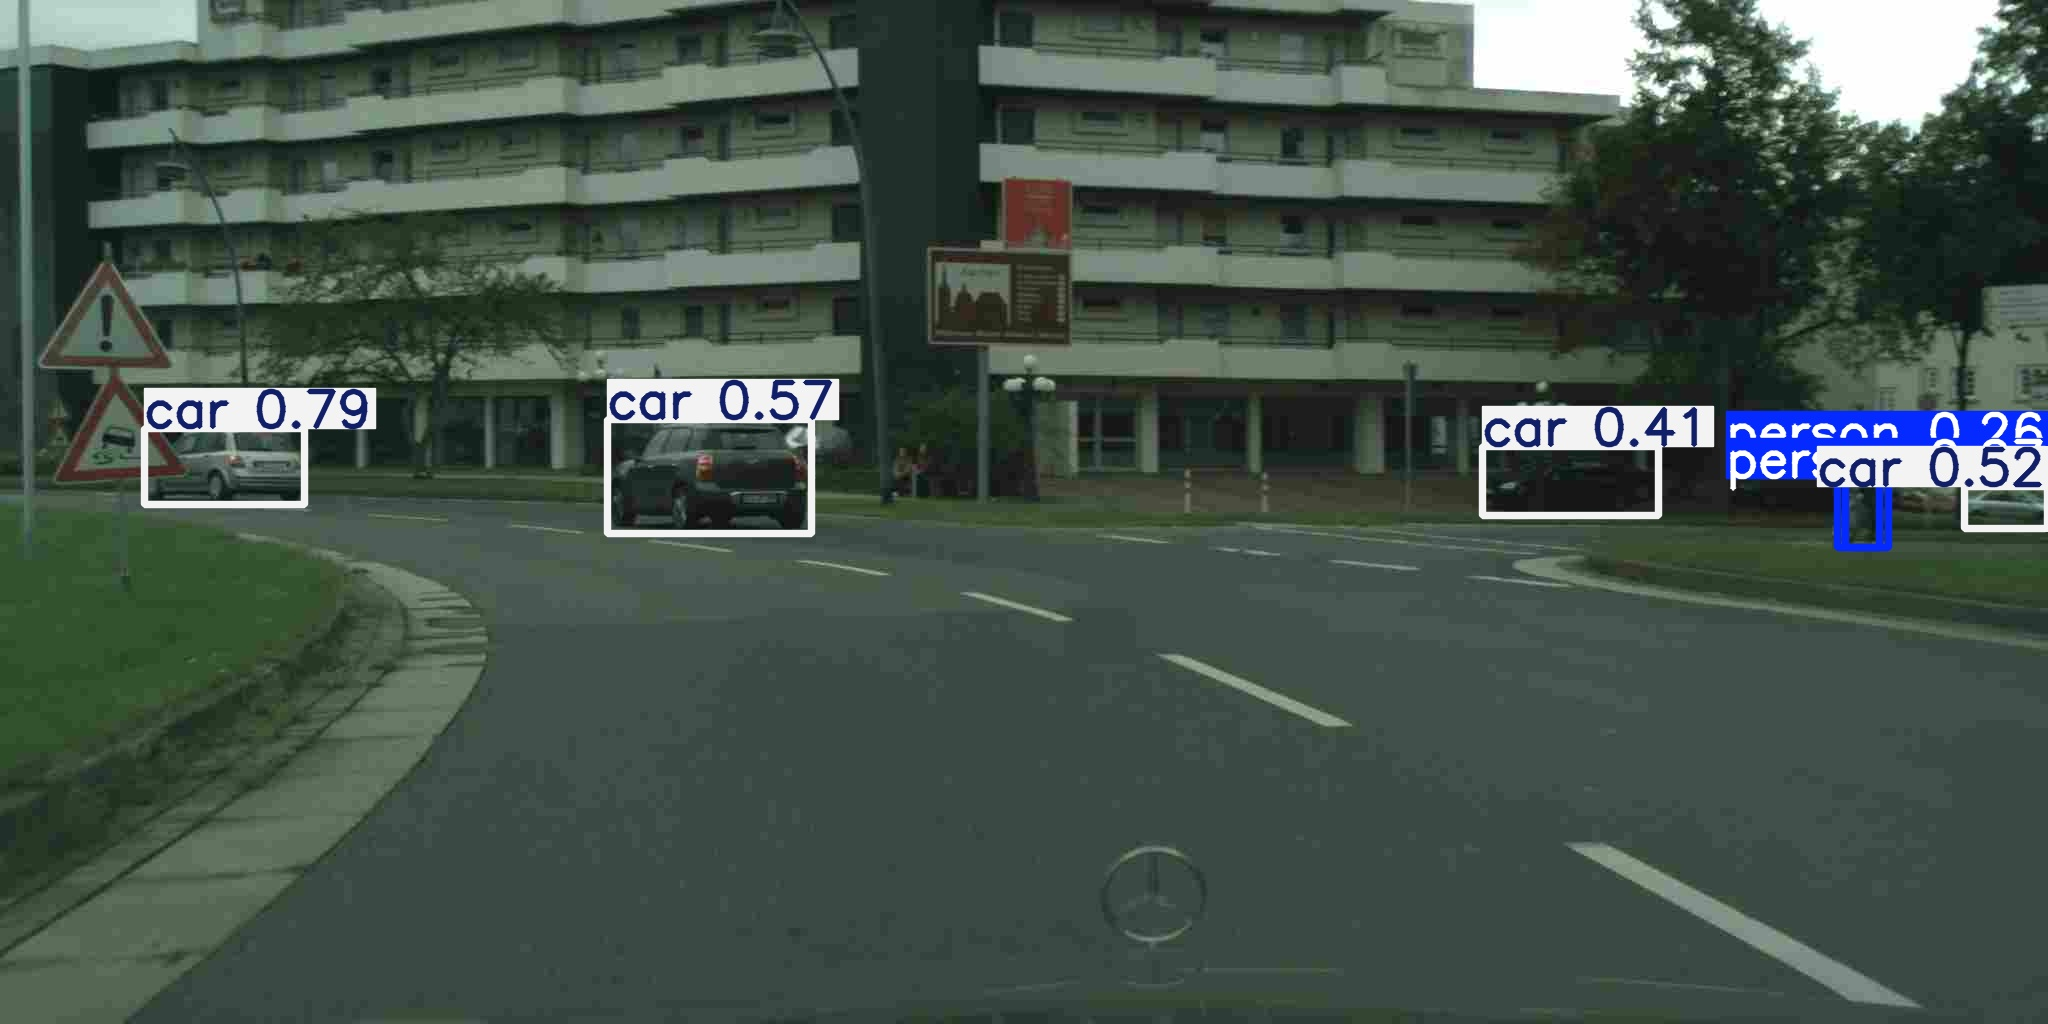
\includegraphics[scale=0.19]{pictures/jpg15_aachen_000000.jpg}
                \caption{Bild mit einer Kompressionsqualität von $15\%$ (Aachen, erstes Bild) zur Objekterkennung mit dem YOLO-Modell.}
                \label{fig:15_aachen_000000}
            \end{figure}
\newpage
            \begin{figure}[!htb]
                \centering
                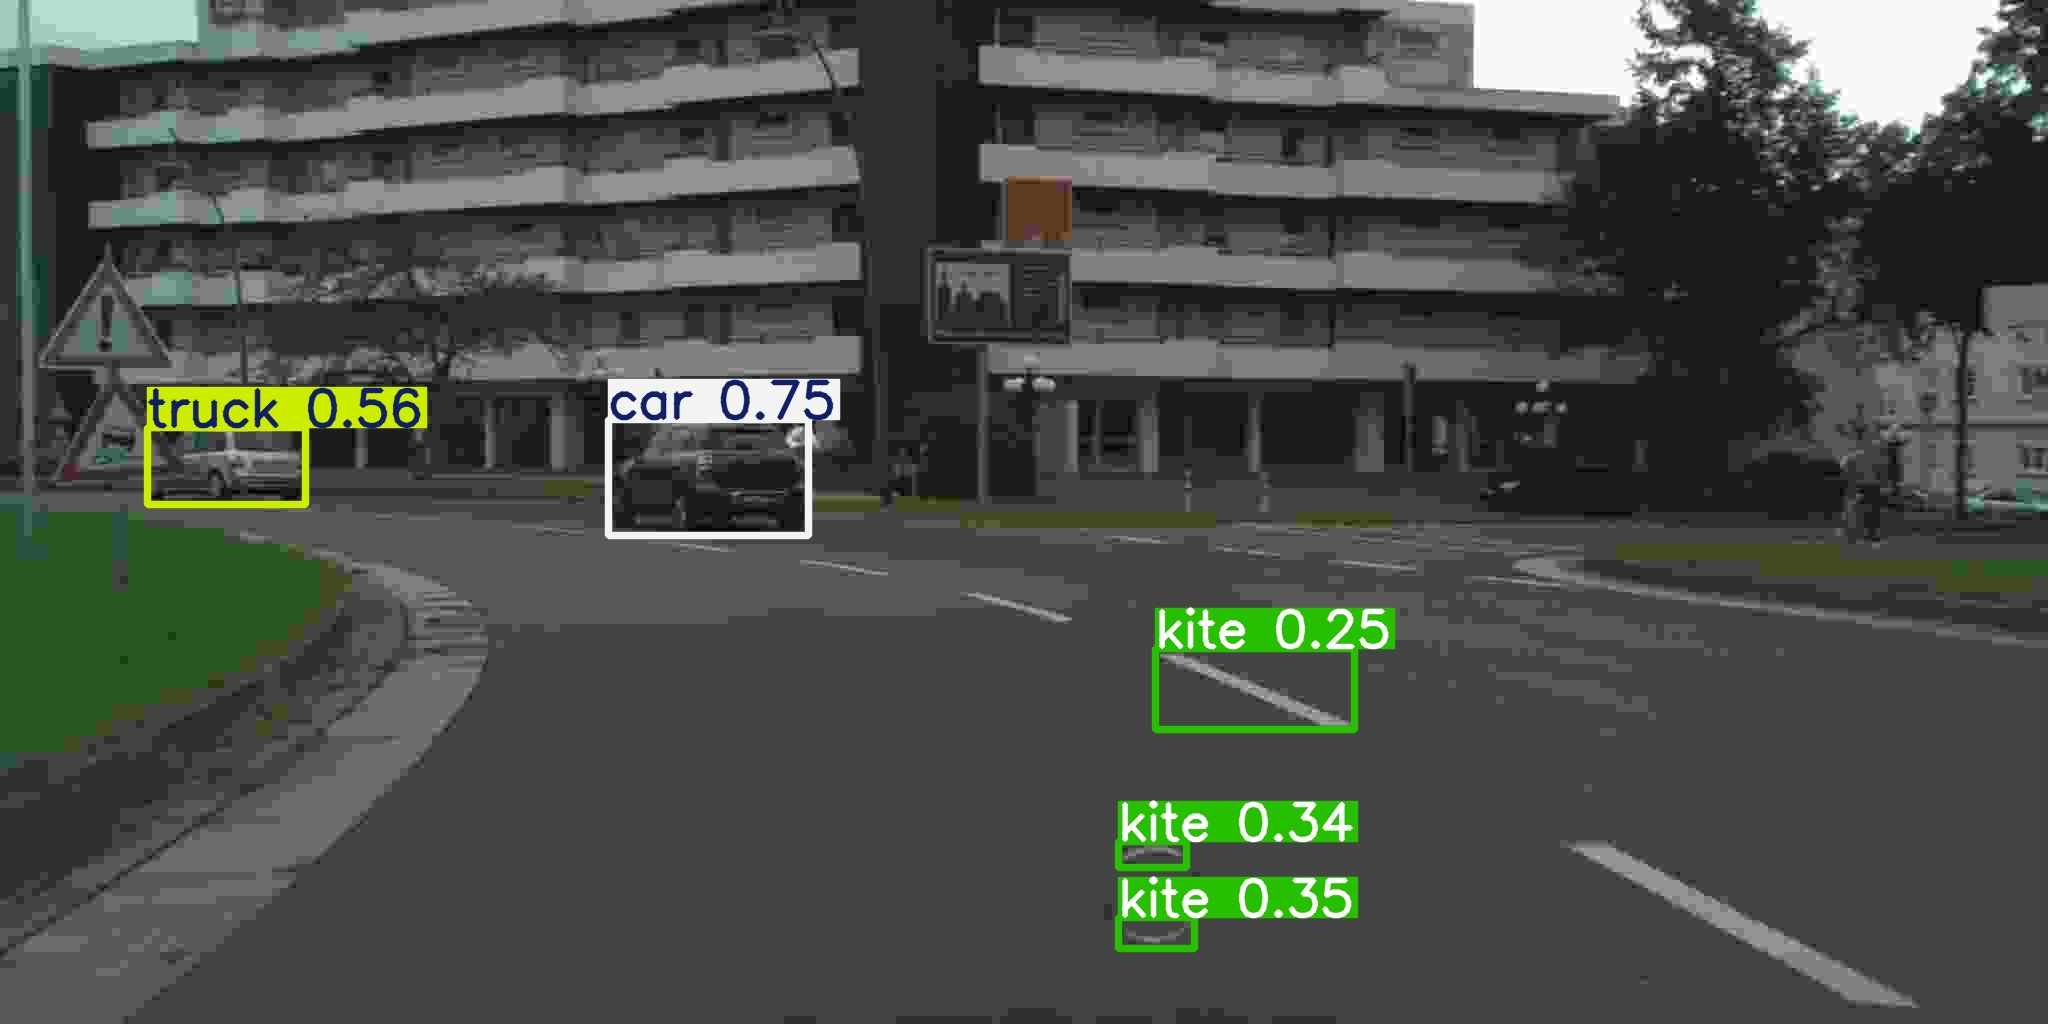
\includegraphics[scale=0.19]{pictures/jpg5_aachen_000000.jpg}
                \caption{Bild mit einer Kompressionsqualität von $5\%$ (Aachen, erstes Bild) zur Objekterkennung mit dem YOLO-Modell.}
                \label{fig:5_aachen_000000}
            \end{figure}

            Mit abnehmender Bildqualität werden Objekte undeutlicher, was das Erkennen von Objekten erheblich erschwert. Die prozentualen Wahrscheinlichkeiten der Klassifizierung sinken, wie in den Abbildungen \ref{fig:90_aachen_000000} und \ref{fig:15_aachen_000000} gut zu sehen ist. Dies führt dazu, dass Objekte entweder gar nicht erkannt oder falsch klassifiziert werden. Aufgrund der mangelnden Bildqualität werden teilweise sogar neue Objekte erkannt, wie in Abbildung \ref{fig:5_aachen_000000} „kite“.
            Dies lässt auf einen kausalen Zusammenhang schließen, dass Bilder mit schlechterer Qualität für eine Objektdetektion auch schlechter abschneiden. 
            Durch die abnehmende Bildqualität entstehen Fragmente sowie farblich falsche Kontraste, Helligkeits- und Sättigungswerte, wie deutlich in Abbildung \ref{fig:5_aachen_000000} zu sehen ist. Das Auto, welches in jedem der drei Bilder erkannt wird, weist verschiedene Wahrscheinlichkeiten auf, zur Klasse „Car“ zu gehören – und dies nicht in einer klar absteigenden Reihenfolge in Abhängigkeit von der Bildqualität.
            Im Originalbild (Abbildung \ref{fig:og_aachen_000000}) liegt die Wahrscheinlichkeit bei $77\%$. Bei dem Bild mit einer Kompressionsqualität von $90\%$ (Abbildung \ref{fig:90_aachen_000000}) steigt die Wahrscheinlichkeit auf $82\%$. In Abbildung \ref{fig:15_aachen_000000} sinkt die Wahrscheinlichkeit, wie man es bei einem Bild mit schlechterer Qualität erwarten würde, auf $57\%$. Erstaunlicherweise erreicht das Bild mit lediglich $5\%$ Kompressionsqualität (Abbildung \ref{fig:5_aachen_000000}) fast die gleiche Wahrscheinlichkeit wie das Originalbild, nämlich $75\%$.
            Dies zeigt, dass auch das Modell eine Rolle spielt, das die Objekte erkennen soll und hat ebenso wie die Qualität des Bildes einen Einfluss darauf, wie gut Objekte erkannt werden. Dies gilt trotz der Tatsache, dass die Labels und die komprimierten Datensätze alle mit demselben Modell erstellt wurden.\\
            \textbf{Kompressionsqualität $5\%$}:\\
            $\text{true positives} = 1 \quad \text{false positives} = 4 \quad \text{false negatives} = 7$
            
\newpage   
            \begin{figure}[!htb]
                \centering
                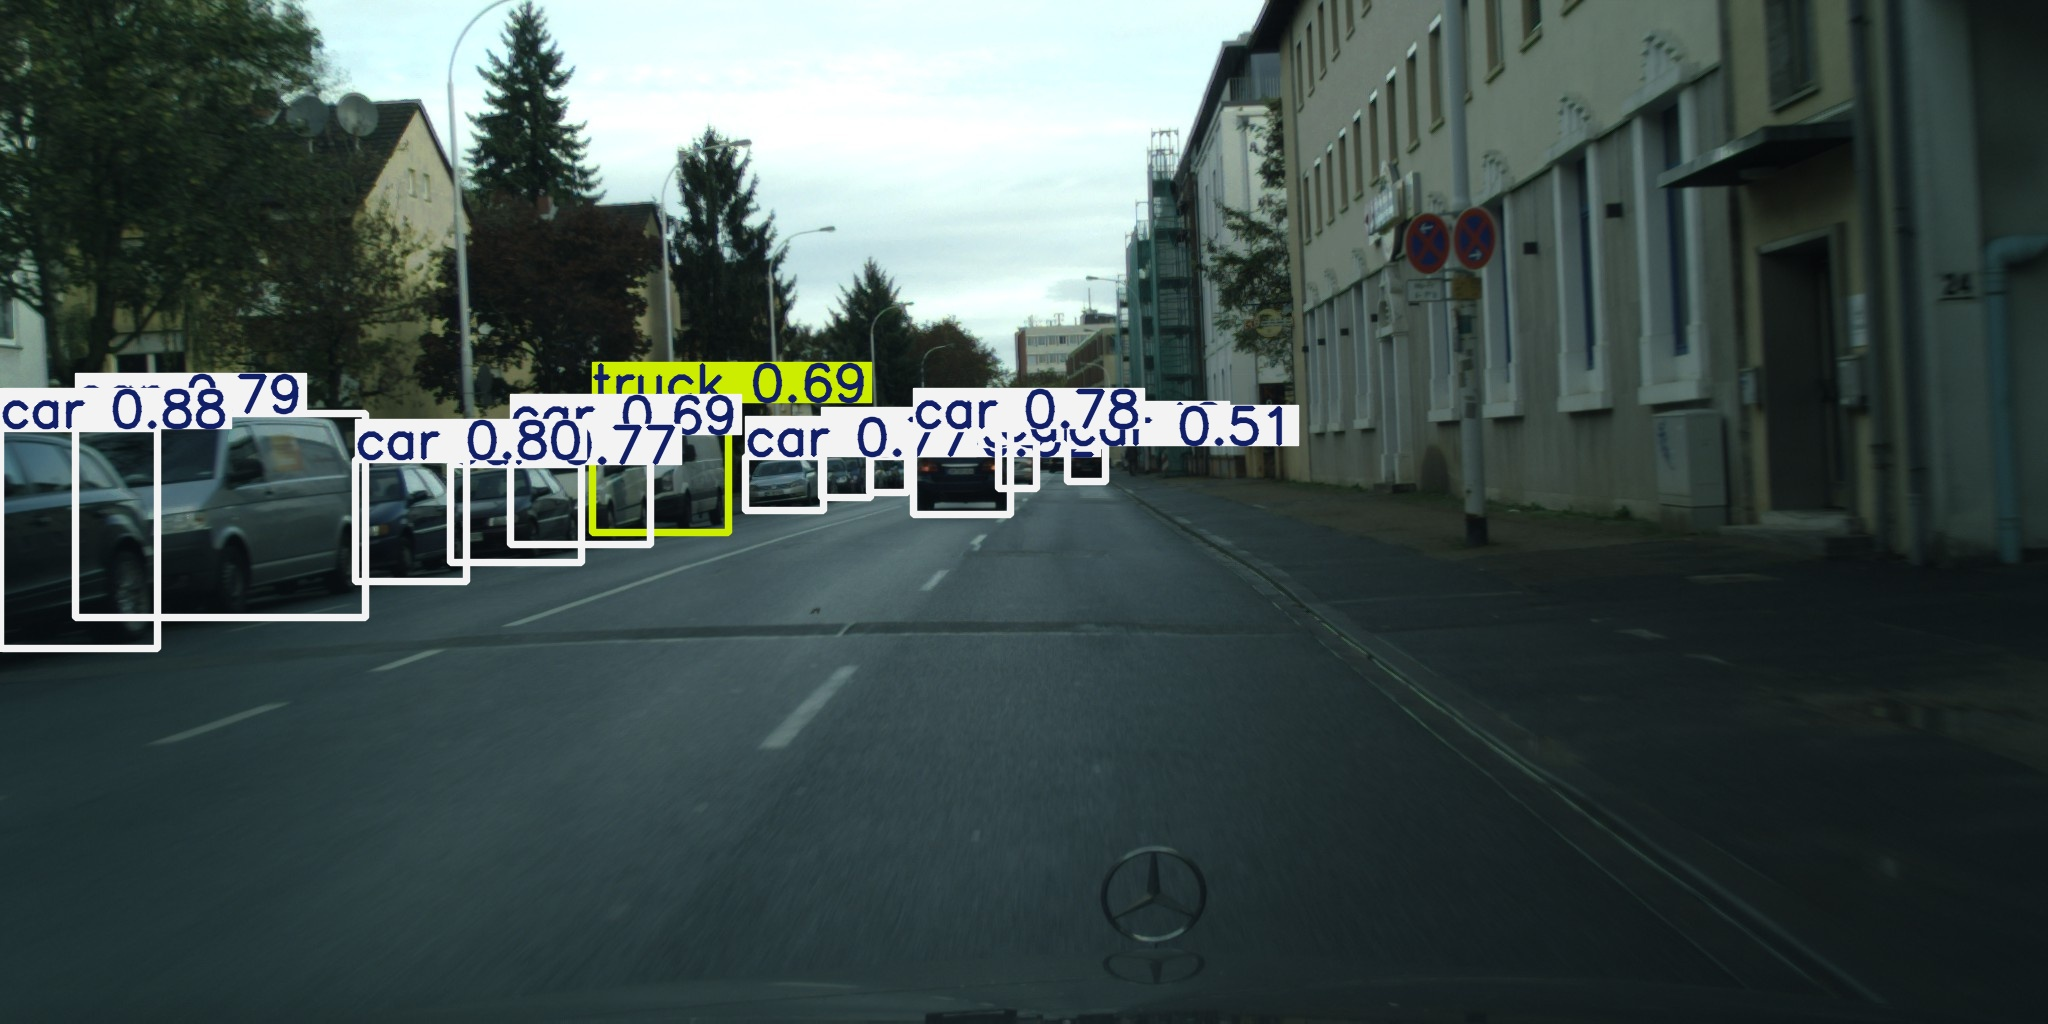
\includegraphics[scale=0.19]{pictures/jpg90_darmstadt_000000.jpg}
                \caption{Bild aus dem Cityscapes-Datensatz mit einer JPEG-Kompressionsqualität von $90\%$ (Darmstadt, erstes Bild), verarbeitet zur Objekterkennung durch das YOLO-Modell.}
                \label{fig:90_darmstadt_000000}
            \end{figure}
            \begin{figure}[!htb]
                \centering
                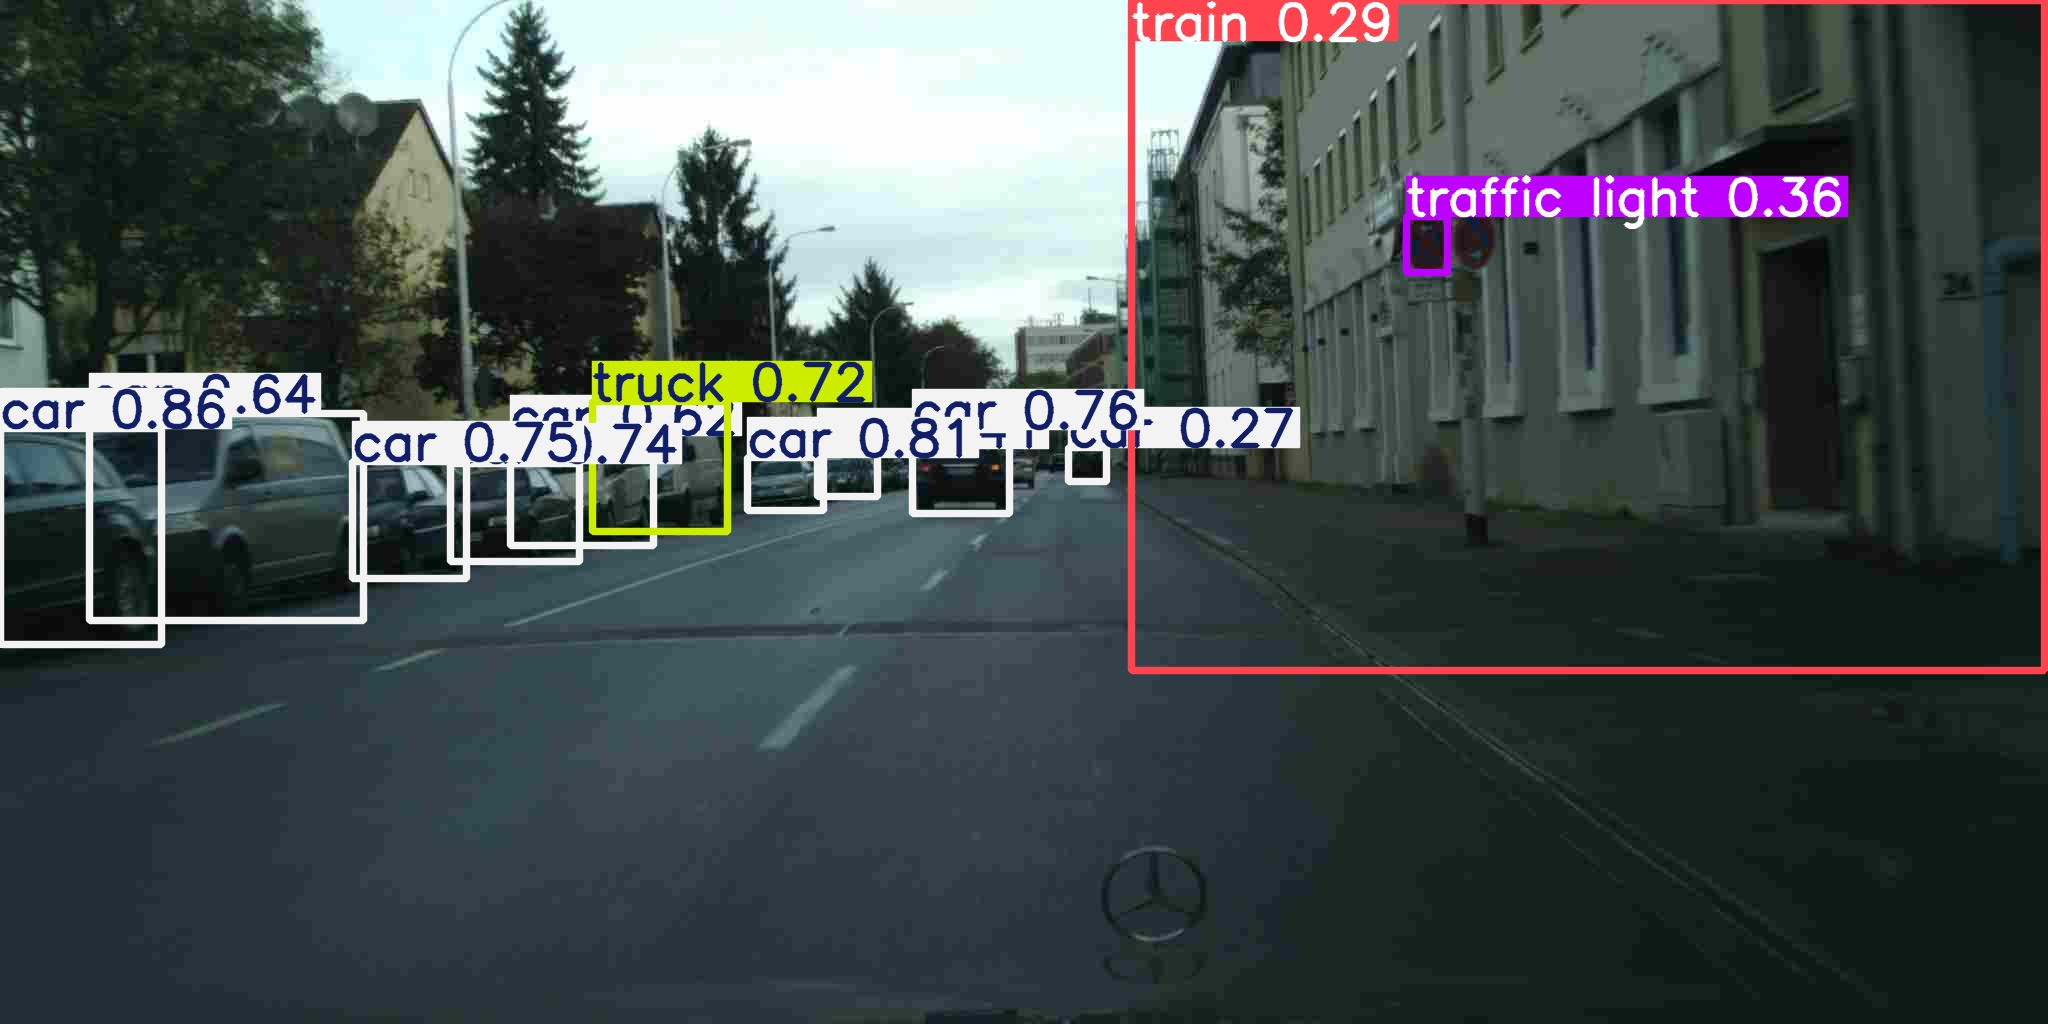
\includegraphics[scale=0.19]{pictures/jpg15_darmstadt_000000.jpg}
                \caption{Bild aus dem Cityscapes-Datensatz mit einer JPEG-Kompressionsqualität von $15\%$ (Darmstadt, erstes Bild), verarbeitet zur Objekterkennung durch das YOLO-Modell.}
                \label{fig:15_darmstadt_000000}
            \end{figure}

\newpage    
            \begin{figure}[!htb]
                \centering
                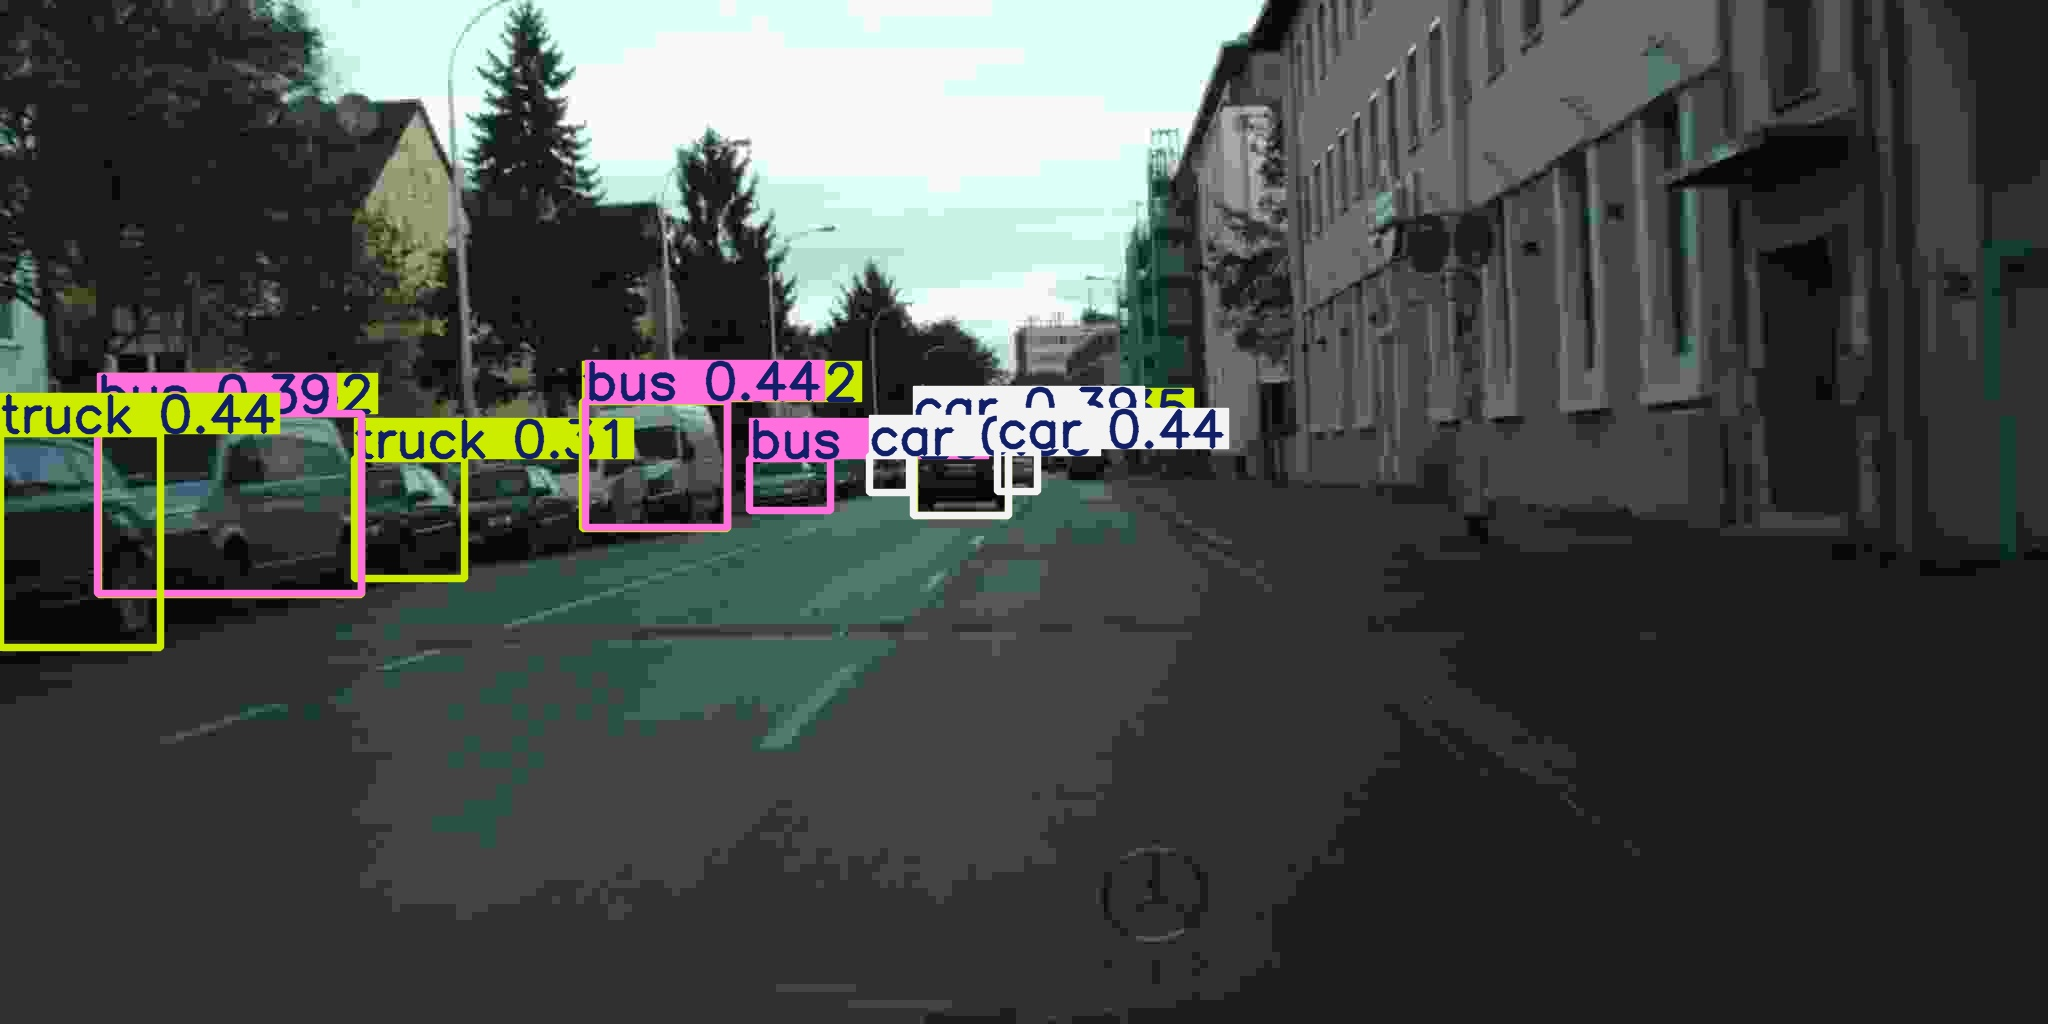
\includegraphics[scale=0.19]{pictures/jpg5_darmstadt_000000.jpg}
                \caption{Bild aus dem Cityscapes-Datensatz mit einer JPEG-Kompressionsqualität von $5\%$ (Darmstadt, erstes Bild), verarbeitet zur Objekterkennung durch das YOLO-Modell.}
                \label{fig:5_darmstadt_000000}
            \end{figure}

            Auch auf den Darmstadt-Bildern in den Abbildungen \ref{fig:90_darmstadt_000000}, \ref{fig:15_darmstadt_000000} und \ref{fig:5_darmstadt_000000} ist deutlich zu erkennen, wie die Objektdetektion bei abnehmender Qualität darunter leidet. So wurde beispielsweise in Abbildung \ref{fig:15_darmstadt_000000} eine ganze Häuserfassade fälschlicherweise als Zug klassifiziert. Auffällig ist außerdem, dass gewöhnliche Autos bei geringerer Qualität häufig als „truck“ oder „bus“ falsch klassifiziert werden.
            Diese Fehlklassifizierung der Autos tritt bei jedem Bild auf, sobald die Kompressionsqualität zu
            gering wird und die Artefakte im Bild deutlich zu erkennen sind.
            Dies liegt jedoch am YOLO-Modell. „truck“, „bus“ und „car“ müssen ähnliche Merkmalsrepräsentationen aufweisen.
            YOLO11 ist ein CNN und verwendet Feature Maps, die Muster aus Bildern extrahieren. Wenn „truck“, „bus“ und „car“ ähnliche Werte aufweisen, bedeutet das, dass ihre Merkmale (z.B. Kanten, Konturen, Formen) sich stark überschneiden.
            

\newpage  
            \underline{\textbf{Metriken zum Vergleich von Bildern mit Labels}}        
            \begin{figure}[!htb]
                \centering
                \includesvg[scale=0.56]{graphs/output_plot_f1_pr_re.svg}
                \caption{Diese Grafik zeigt die Metriken Precison, Recall und F1 Score in Abhängigkeit zur Kompressionsqualität.}
                \label{fig:pr_f1_re}
            \end{figure}

            Der F1-Score sowie Precision und Recall sind gängige Metriken zur Überprüfung,
            wie gut ein Modell einen Datensatz auf die dazugehörigen Labels abbildet und klassifiziert.
            Es ist zu erkennen, dass bei einer Kompressionsqualität von $85\%$–$100\%$ die drei Metriken nahe bei 1,0 liegen (1,0 entspräche den Originaldaten). Precision verläuft dabei sehr flach – flacher als Recall und der F1-Score. Mit einer nahezu null Steigung bleibt sie bis zu einer Kompressionsqualität von etwa $25\%$–$30\%$ konstant. Erst unterhalb dieser Werte beginnt die Kurve erkennbar abzufallen.
            Dies haben alle drei Metriken gemeinsam: Sie fallen ab, sobald die Kompressionsqualität unterhalb dieser Werte sinkt. Die Kurven spiegeln das wider, was man in den Bildern mit verschiedenen Kompressionsqualitäten bereits sehen konnte.   
            Die Differenz der $y$-Werte (Metriken-Scores) bei gleicher $x$-Werte (Kompressionsqualität) nimmt zu, je geringer die Kompressionsqualität wird. Die drei Kurven starten bei $100\%$ nahezu am selben Punkt und driften vom F1-Wert zunehmend ab.
            Bis zu Werten von $75\%$ weichen Precision und Recall maximal um $y = \pm 0,02$ vom F1-Score ab. Über einen Bereich von $x = 50$ Einheiten hinweg steigen die Abweichungen maximal auf $y = \pm 0,03$. Erst unterhalb von $30\%$ driften die Kurven stark auseinander. Bei $x = 5$ erreichen Precision $y = +0,2$ und $y = -0,1$ für Recall, abweichend vom F1-Score.
            
\newpage            
            \begin{figure}[!htb]
                \centering
                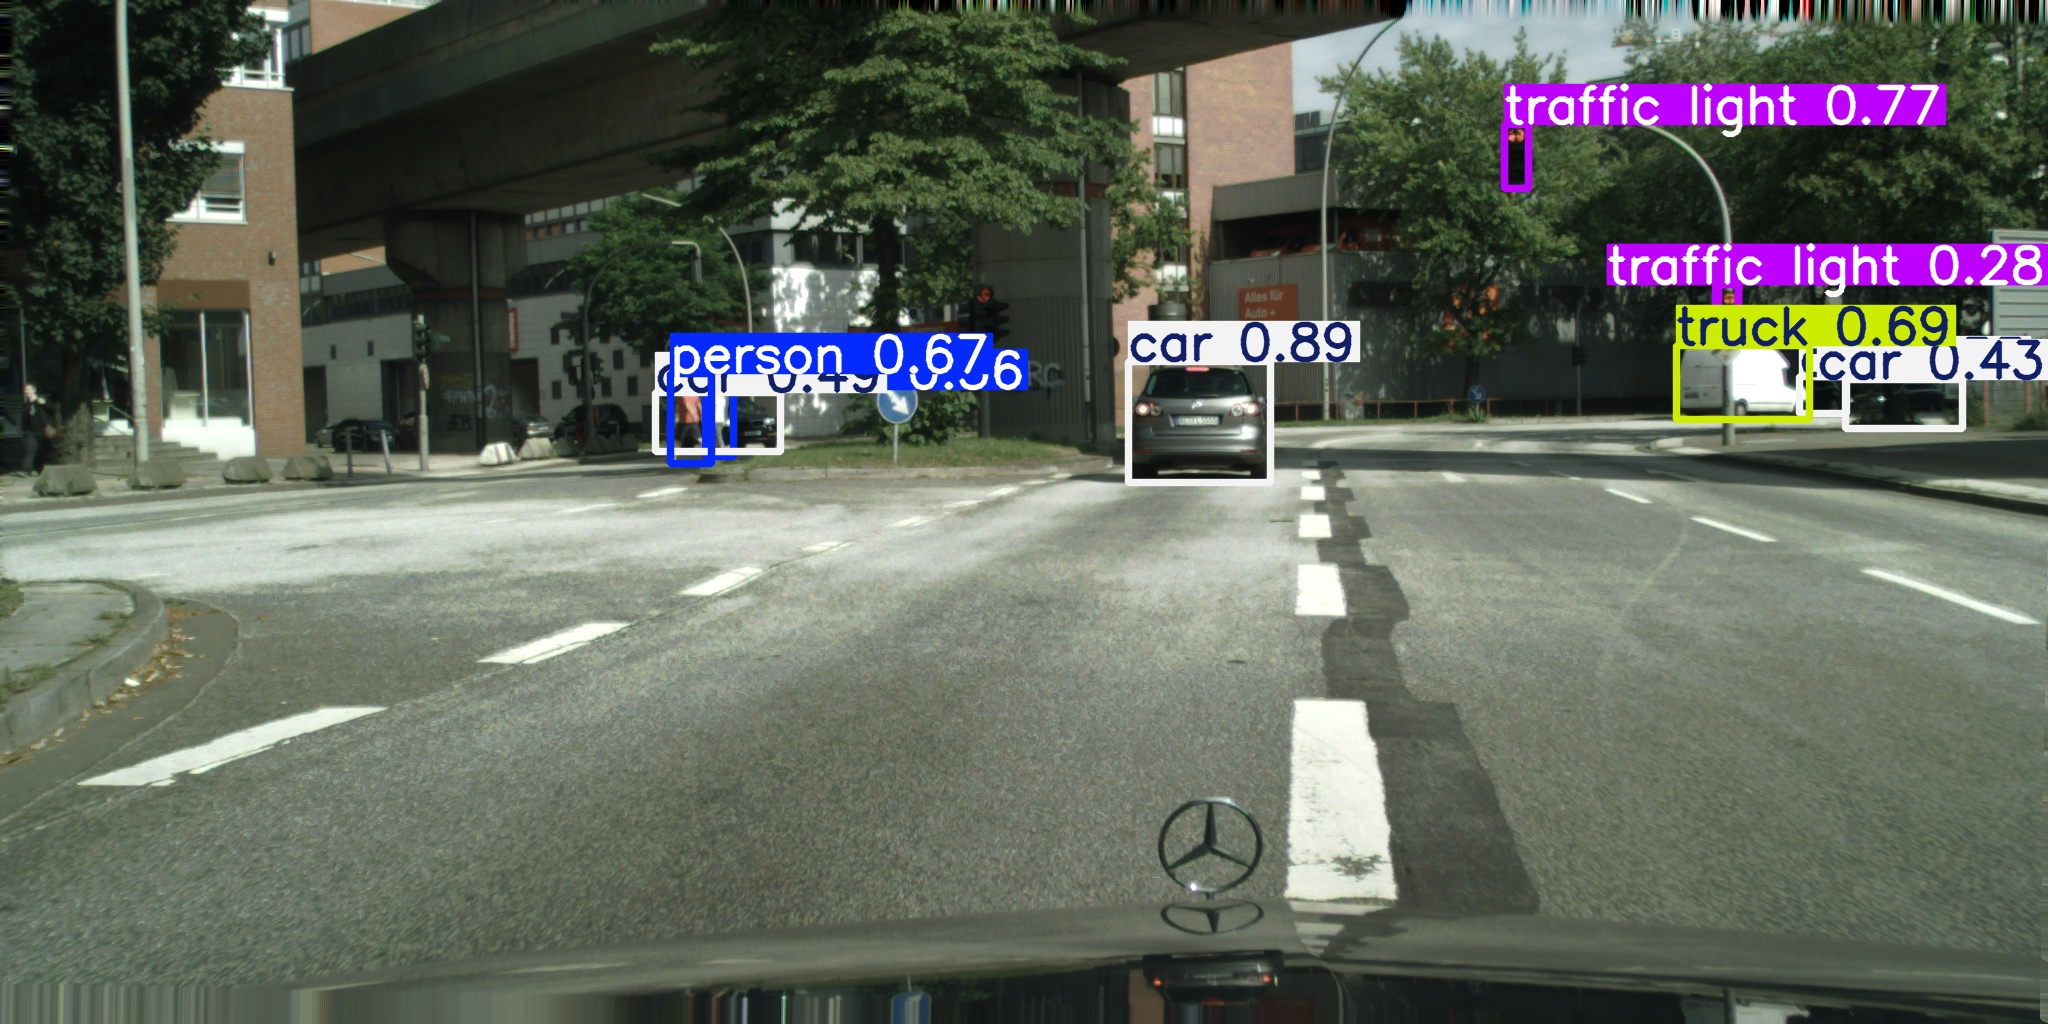
\includegraphics[scale=0.19]{pictures/original_hamburg_000000.jpg}
                \caption{Original Label Bild aus dem Cityscapes Datensatz (Hamburg sechstes Bild) zur Objekterkennung durch das YOLO- Model.}
                \label{fig:og_hamburg_6}
            \end{figure}
            \begin{figure}[!htb]
                \centering
                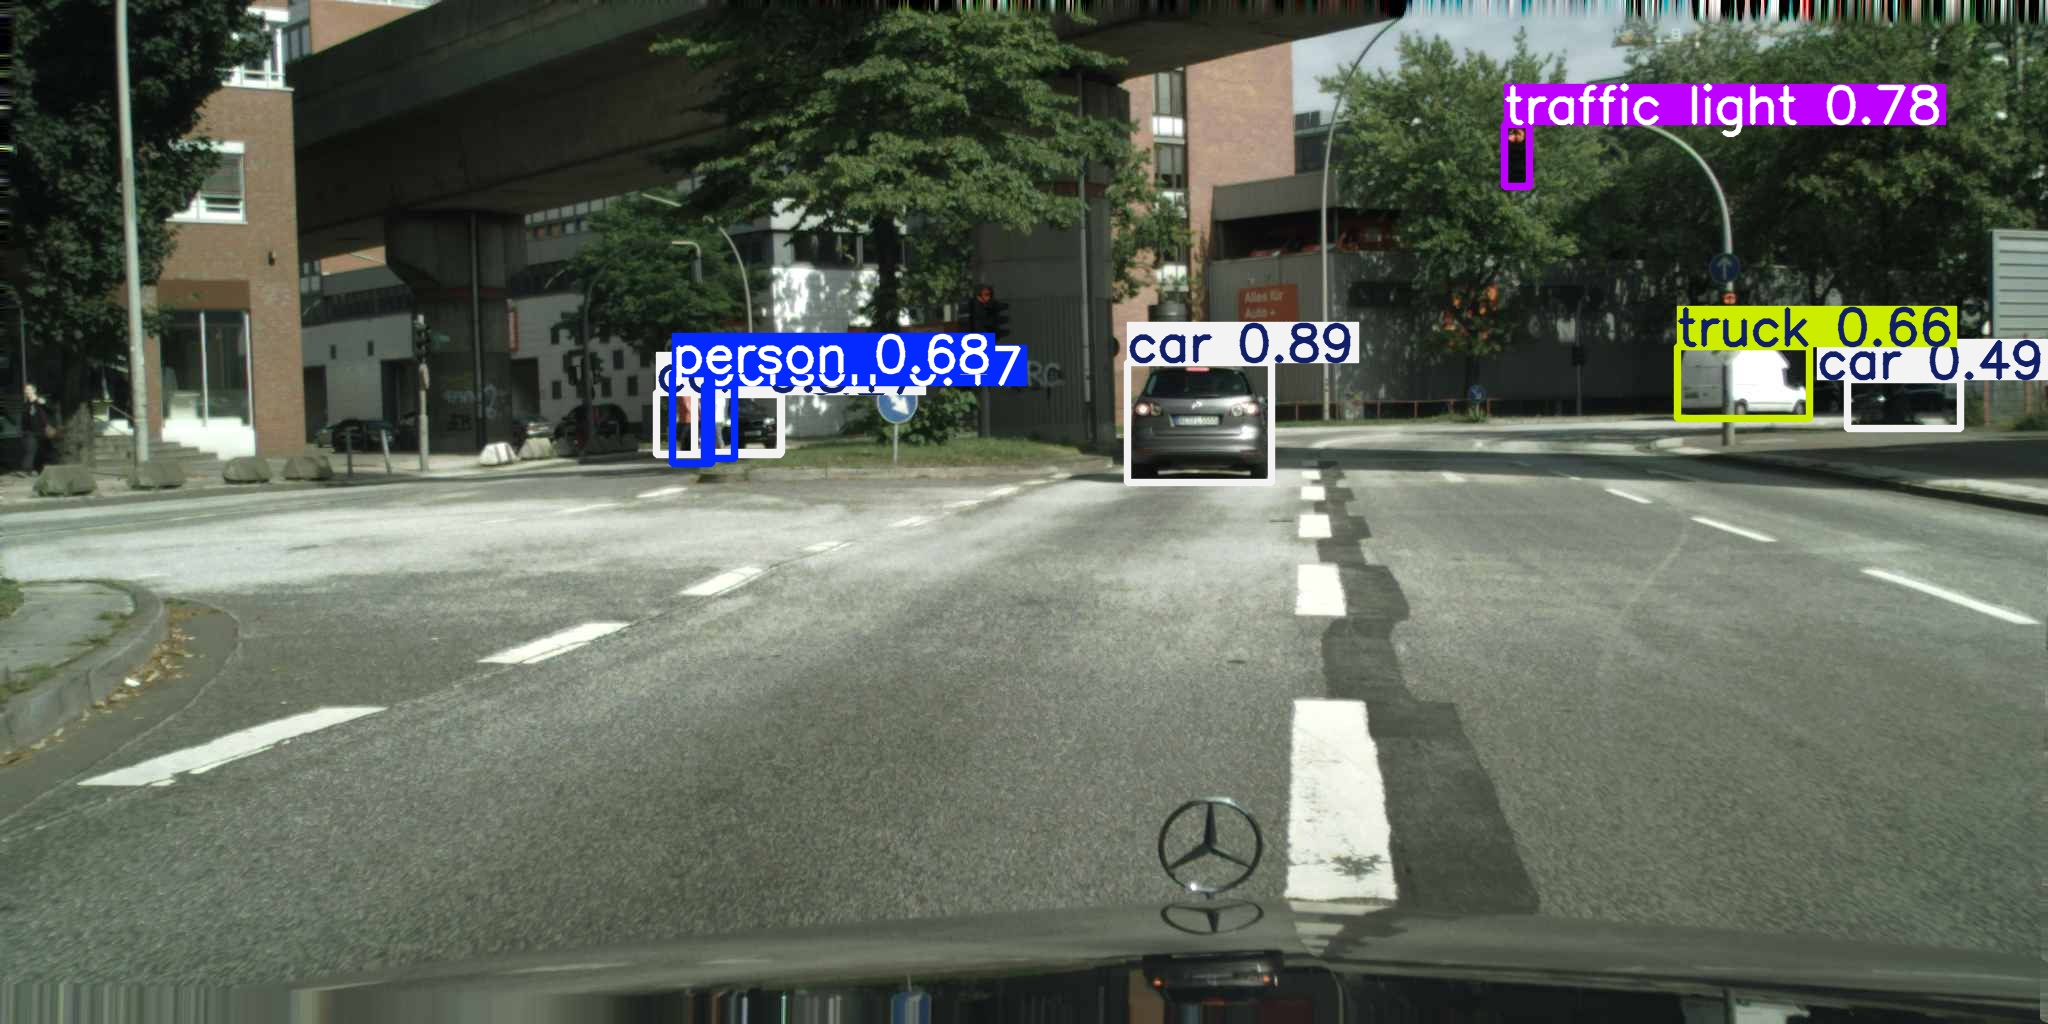
\includegraphics[scale=0.19]{pictures/jpg40_hamburg_000000.jpg}
                \caption{Bild aus dem Cityscapes-Datensatz mit einer JPEG-Kompressionsqualität von $40\%$ (Hamburg, sechstes Bild), verarbeitet zur Objekterkennung durch das YOLO-Modell.}
                \label{fig:jpg40_hamburg_6}
            \end{figure}
\newpage
            
            \begin{figure}[!htb]
                \centering
                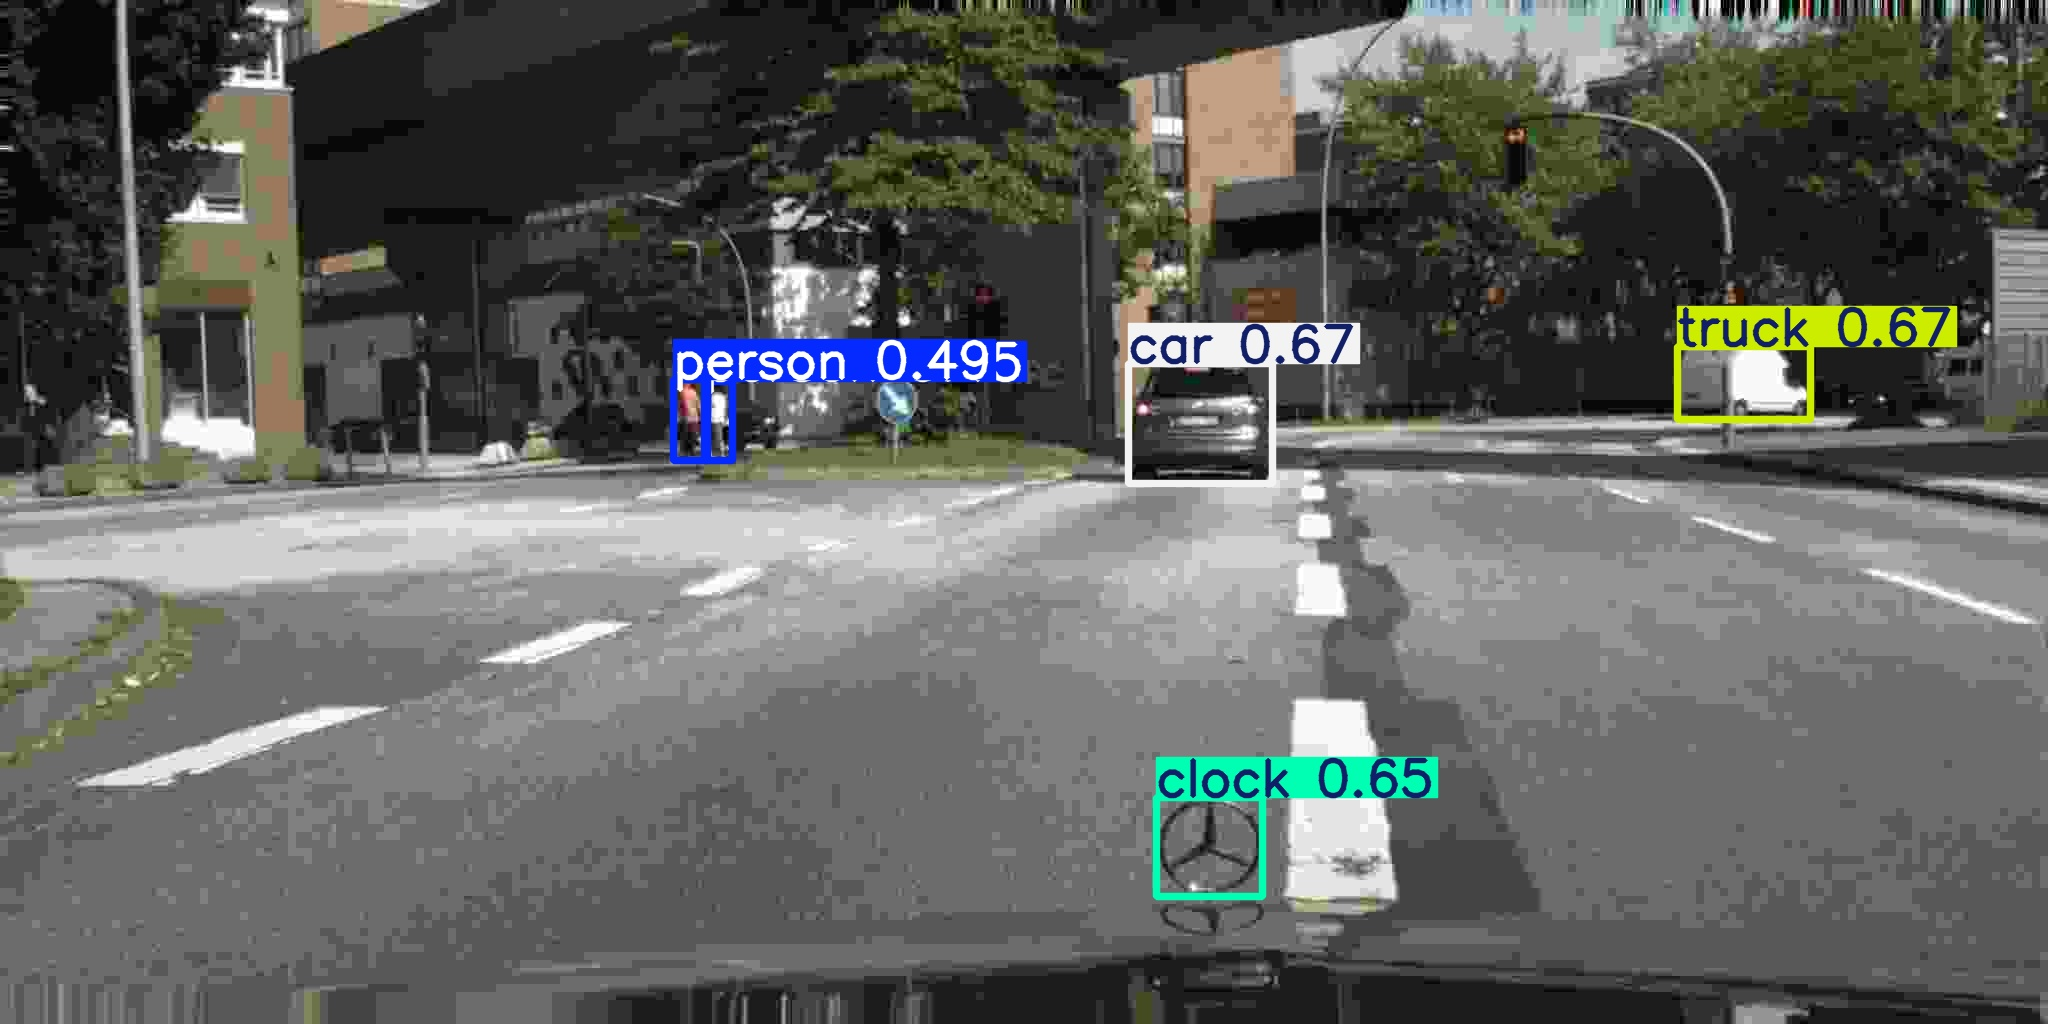
\includegraphics[scale=0.19]{pictures/jpg5_hamburg_000000.jpg}
                \caption{Bild aus dem Cityscapes-Datensatz mit einer JPEG-Kompressionsqualität von $5\%$ (Hamburg, sechstes Bild), verarbeitet zur Objekterkennung durch das YOLO-Modell.}
                \label{fig:jpg5_hamburg_6}
            \end{figure}

            Bei den Bildern aus Hamburg sieht man, dass die Grafik \ref{fig:pr_f1_re} die Ergebnisse korrekt darstellt, da kaum ein Unterschied in der Objektdetektion zwischen \ref{fig:jpg40_hamburg_6} und \ref{fig:og_hamburg_6} erkennbar ist – abgesehen von einem fehlenden „traffic light“. Auffällig ist zudem, dass in Abbildung \ref{fig:jpg5_hamburg_6} bei einer Kompressionsqualität von $5\%$ die Klassifizierung des „Truck“ mit einem Wert von $67\%$ angegeben wird, was $1\%$ höher ist als bei einer Kompressionsqualität von $40\%$ in Abbildung \ref{fig:jpg40_hamburg_6}.
            Dies lässt erneut darauf schließen, dass nicht nur der Grad der Komprimierung, sondern auch das Modell zur Objektdetektion selbst eine Rolle dabei spielt, wie gut ein Objekt auf qualitativ schlechteren Bildern erkannt wird.
            Auch ist hier zu sehen, dass der Mercedes-Stern als „clock“ klassifiziert wird. Da alle Datensätze auch die Labels mit demselben Modell für die Boundingboxen erstellt wurden, wäre zu erwarten gewesen, dass ein Bild besserer Qualität, wie das Label, an dieser Stelle ebenfalls als „clock“ klassifiziert worden wäre, was jedoch nicht der Fall ist. 
            Dies zeigt, dass durch mangelnde Bildqualität Fehlklassifizierungen entstehen.
            
\newpage  
            \underline{\textbf{Intersection over Union (IoU)}}\bigskip
            
            Um die Qualität der Bounding-Boxen zu überprüfen und zu bewerten, inwieweit sie mit den Ground-Truth-Boundingboxen übereinstimmen, wird der IoU verwendet.
            
            \begin{figure}[!htb]
                \centering
                \includesvg[scale=0.56]{graphs/output_plot_iou.svg}
                \caption{IoU in Abhängigkeit zur Kompressionsqualität.}
                \label{fig:iou}
            \end{figure}
            Auch der IoU liegt anfangs von $100\%$ bis zu einer Kompressionsqualität von $25\%$ in guten Wertebereichen oberhalb von $0,8$ teils $0,9$. Unterhalb von $25\%$ fällt der IoU ab auf $0,5$ bei $5\%$ Kompressionsqualität. Der IoU weist innerhalb von $20$ Einheiten auf der $x$-Achse von $5\%$ bis $25\%$ eine Differenz von $0,35$ auf. Von $25\%$ bis $100\%$ über $75$ Einheiten hinweg ist lediglich eine Differenz von $0,17$ Einheiten vorhanden. Dies zeigt erneut den Qualitätsunterschied von Bildern oberhalb der JPEG-Kompressionsqualität von $25\%$ bis $30\%$ und derer, die darunter liegen. Diese Gemeinsamkeit weisen alle Metriken auf, welche in dieser Arbeit betrachtet werden, dass unterhalb dieser Schwellwerte sich die Werte deutlich verschlechtern.
            Bei näherer Betrachtung zeigt der IoU nahezu identische Kurvenverläufe wie der Recall in Abbildung \ref{fig:pr_f1_re}. Ein Unterschied der beiden Kurven besteht darin, dass der IoU von ($x = 25$, $y = 0,79$) über die nächsten $75$ Einheiten bis zu ($x = 100$, $y = 0,961$) etwas steiler ansteigt. Recall liegt bei ($x = 25$, $y = 0,864$) mit $0,075$ Einheiten über dem IoU und bei ($x = 100$, $y = 0,975$) um $0,014$ Einheit darüber. Auch hier ist bei $50\%$ ein Wendepunkt in der Kurve.
            

\newpage
            \begin{figure}[!htb]
                \centering
                \includesvg[scale=0.56]{graphs/output_plot_iou_std.svg}
                \caption{Diese Grafik zeigt den IoU in Abhängigkeit zur Kompressionsqualität mit Standartabweichung.}
                \label{fig:iou_std}
            \end{figure}
            
            Die Standardabweichung liegt mit $100\%$ Kompressionsqualität noch bei $0,13$, erhöht sich jedoch bis auf $0,44$ bei einer Kompressionsqualität von $5\%$. Die Standardabweichung wird auf den Mittelwert addiert  bzw. subtrahiert. Aufgrund der stark variierenden Werte kann die Summe aus Mittelwert und Standardabweichung auch über $1,0$ liegen, obwohl die einzelnen IoU-Werte immer zwischen $0$ und $1$ liegen. Die einzelnen IoU-Werte reichen von $0,99$ bis hin zu $0,0$.
            Dies liegt daran, dass die Berechnung des IoU einen Schwellenwert (Threshold) hat. Bei Werten unter $0,5$ wird der IoU auf Null gesetzt. Dadurch ergeben sich zahlreiche Werte, die entweder bei Null oder nahe $1,0$ liegen können.\\
\newpage
            \begin{table}[h!]
                \centering
                \begin{tabular}{rl}
                    \toprule
                    \textbf{Index} & \textbf{Wert (gerundet)} \\
                    \midrule
                    1  & 0.9816 \\
                    2  & 0.0 \\
                    3  & 0.9579 \\
                    4  & 0.0 \\
                    5  & 0.0 \\
                    6  & 0.0 \\
                    7  & 0.0 \\
                    8  & 0.0 \\
                    9  & 0.9438 \\
                    10 & 0.9256 \\
                    11 & 0.8562 \\
                    12 & 0.9276 \\
                    13 & 0.7814 \\
                    14 & 0.8782 \\
                    15 & 0.9729 \\
                    16 & 0.0 \\
                    17 & 0.5183 \\
                    18 & 0.8200 \\
                    19 & 0.0 \\
                    20 & 0.9788 \\
                    \bottomrule
                \end{tabular}
                \caption{Die ersten Gerundeten 20 IoU-Werte für eine Kompressionsqualität von $5\%$ (4 Nachkommastellen)}
                \label{tab:compression5}
            \end{table}

            Die ersten 20 IoU-Werte des Datensatzes mit einer Kompressionsqualität von $5\%$ zeigen deutlich, dass die Werte oft weit auseinanderliegen. Dies ist auf den Schwellenwert (Threshold) bei der Berechnung des IoU zurückzuführen: Nur Werte mit $IoU > 0,5$ werden berücksichtigt, während alle darunterliegenden Werte auf $0,0$ gesetzt werden.\\

            \begin{center}
                \underline{Hinweis:}\\
                In die Berechnung des IoU wurden alle Werte einbezogen, die oberhalb des Schwellenwerts (Threshold) liegen, sowie alle Null-Werte (Werte unterhalb des Schwellenwerts), um die tatsächliche Performance des Modells und der Bilder zu untersuchen. Boundingboxen ohne zugehörige Ground-Truth-Boundingbox-Labels und umgekehrt wurden jedoch \textbf{nicht} berücksichtigt und auch \textbf{nicht} als Null-Werte in die Berechnung einbezogen.
            \end{center}
            
\newpage
        \subsection{KI-rekonstruierte Bilder}
            \begin{figure}[!htb]
                \centering
                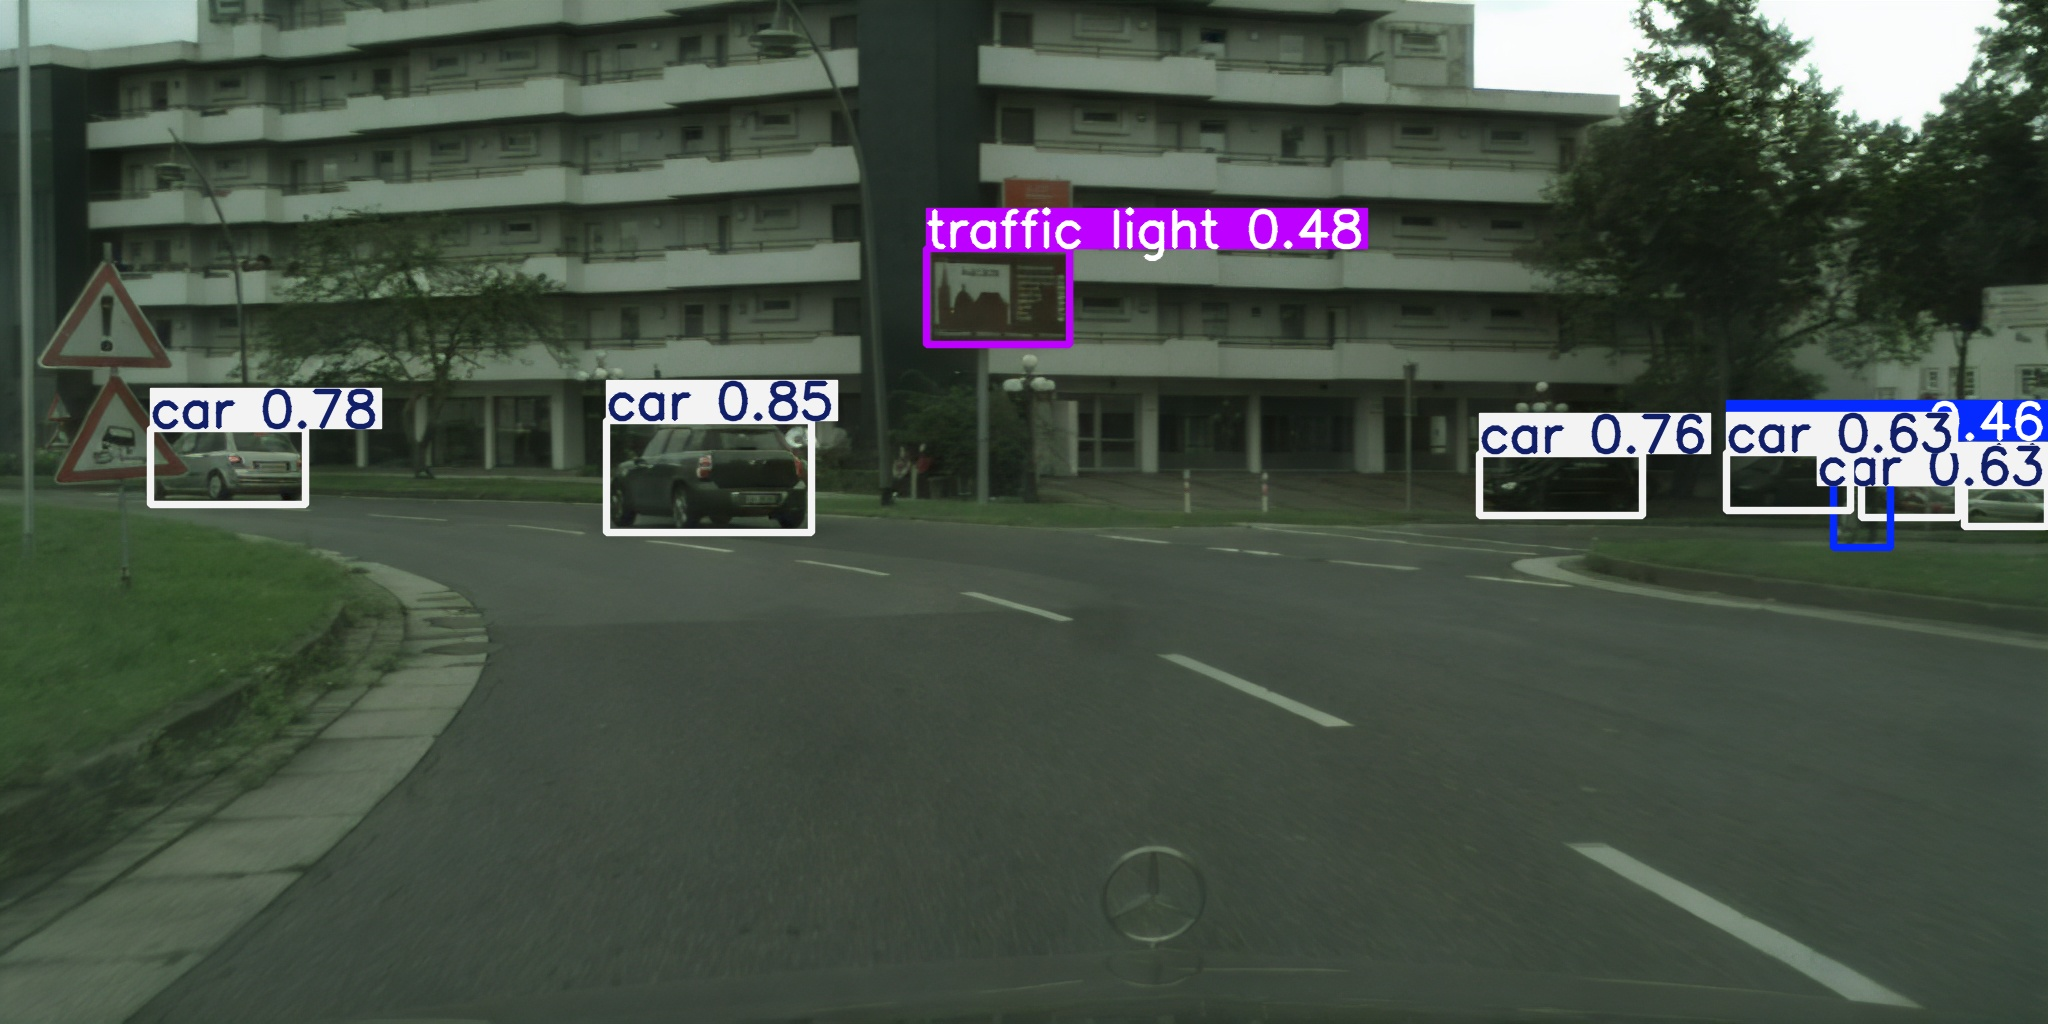
\includegraphics[scale=0.19]{pictures/vq-f8-n256_aachen_000000.jpg}
                \caption{Rekonstruiertes Bild durch das vq-f8-n256-Modell (Aachen, erstes Bild), verarbeitet zur Objekterkennung durch das YOLO-Modell.}
                \label{fig:vq-f8-n256_aachen_000000}
            \end{figure}
            \begin{figure}[!htb]
                \centering
                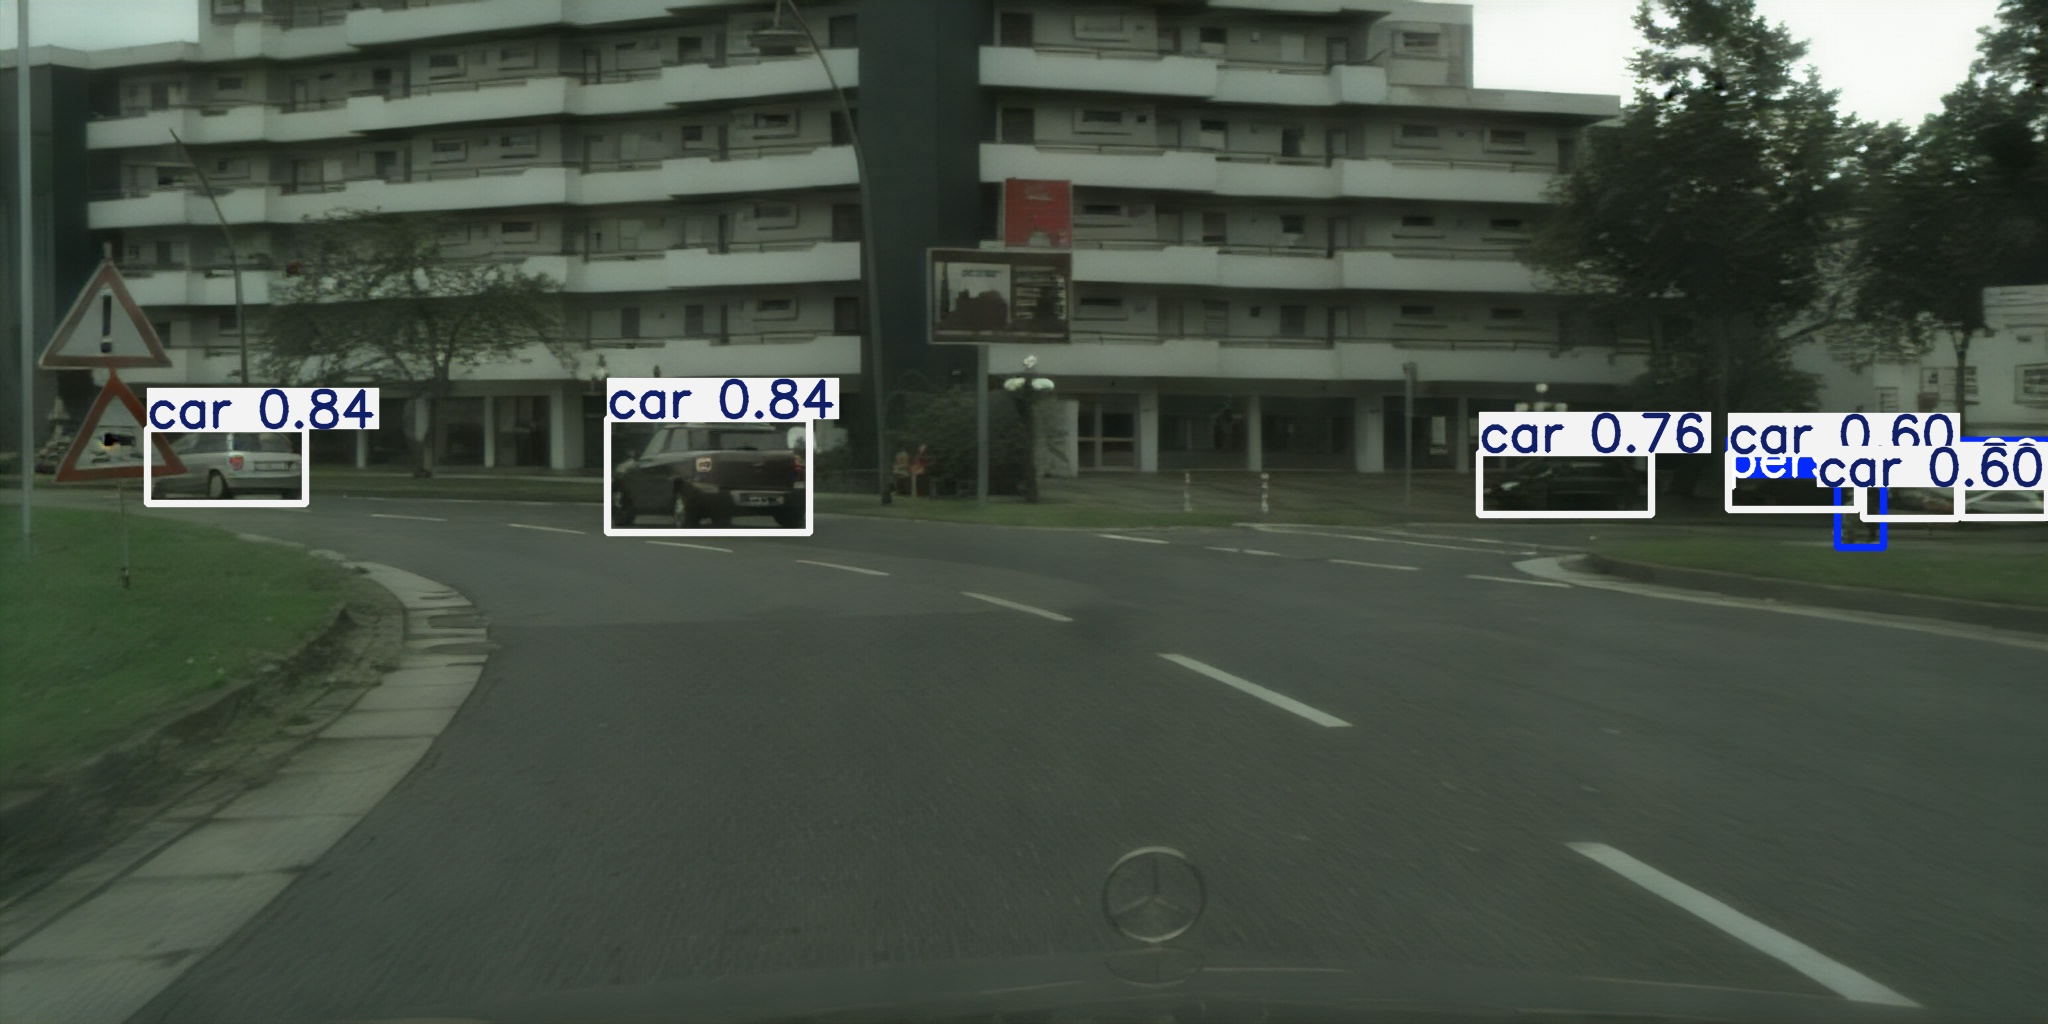
\includegraphics[scale=0.19]{pictures/vq-f16_aachen_000000.jpg}
                \caption{Rekonstruiertes Bild durch das vq-f16-Modell (Aachen, erstes Bild), verarbeitet zur Objekterkennung durch das YOLO-Modell.}
                \label{fig:vq-f16_aachen_000000}
            \end{figure}
\newpage
            \begin{figure}[!htb]
                \centering
                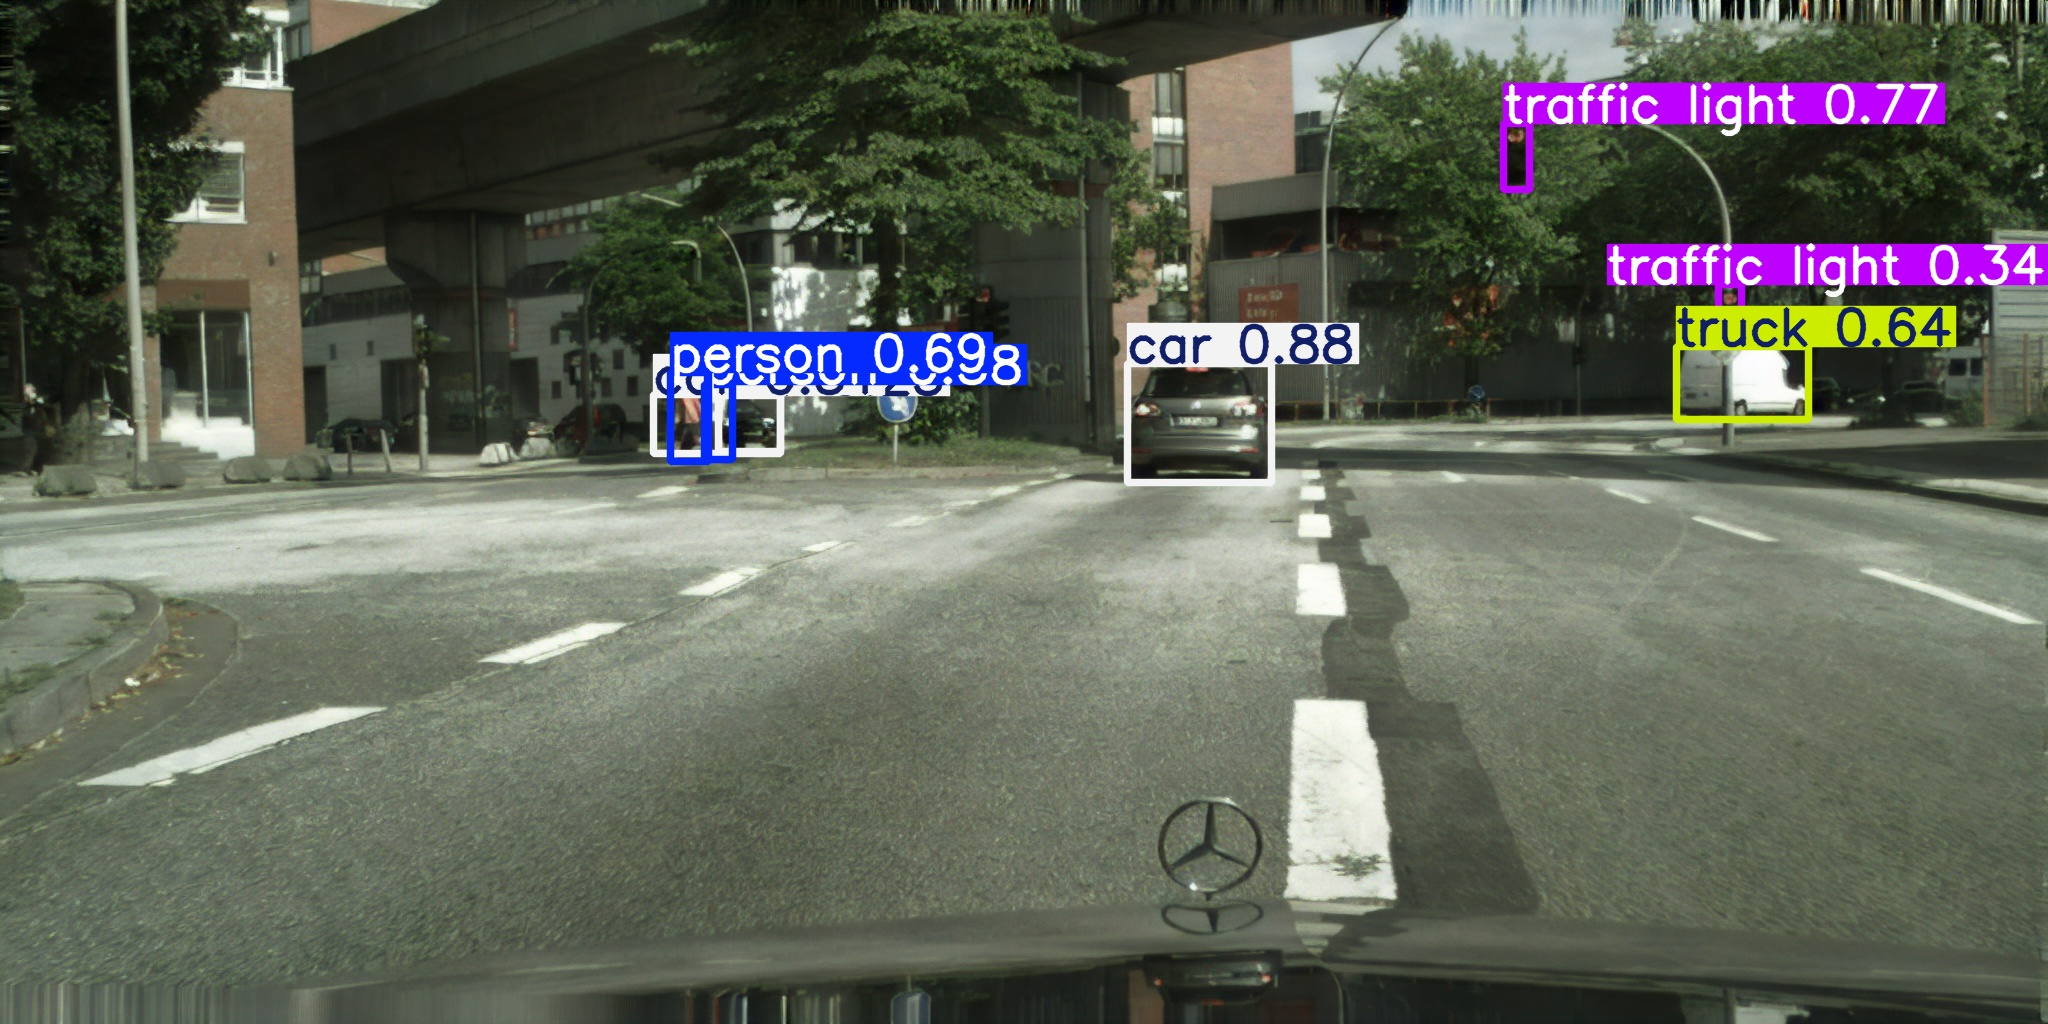
\includegraphics[scale=0.19]{pictures/vq-f8-n256_hamburg_000000.jpg}
                \caption{Rekonstruiertes Bild durch das vq-f8-n256-Modell (Hamburg, sechstes Bild), verarbeitet zur Objekterkennung durch das YOLO-Modell.}
                \label{fig:vq-f8-n256_hamburg_000000}
            \end{figure}
            \begin{figure}[!htb]
                \centering
                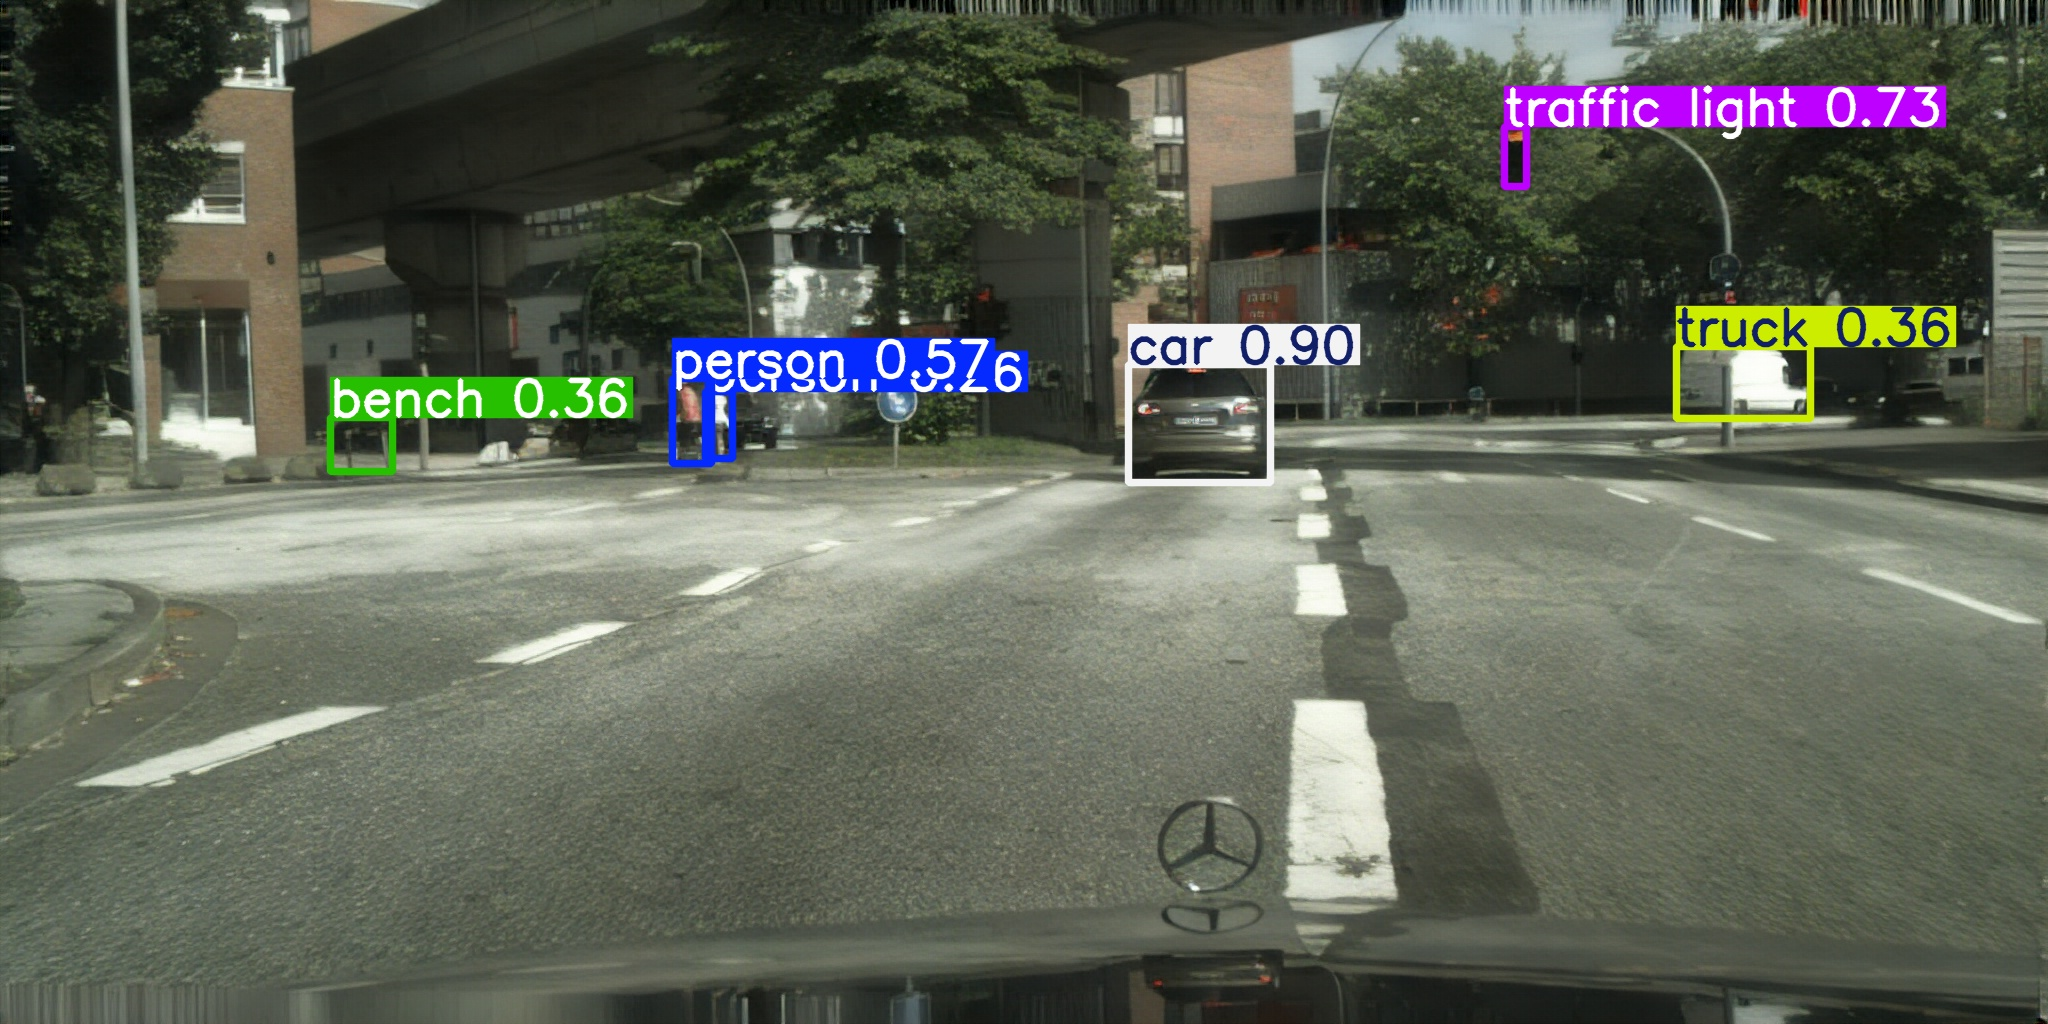
\includegraphics[scale=0.19]{pictures/vq-f16_hamburg_000000.jpg}
                \caption{Rekonstruiertes Bild durch das vq-f16-Modell (Hamburg, sechstes Bild), verarbeitet zur Objekterkennung durch das YOLO-Modell.}
                \label{fig:vq-f16_000000}
            \end{figure}

\newpage
            Auf beiden Aachen-Bildern, Abbildungen \ref{fig:vq-f8-n256_aachen_000000} und \ref{fig:vq-f16_aachen_000000}, werden alle Autos erkannt sowie eine Person. Im Vergleich zum Ground-Truth-Label-Bild
            (Abbildung \ref{fig:og_aachen_000000}) wird auf beiden eine Person nicht erkannt, sowie fälschlicherweise ein Schild als „traffic light“ klassifiziert \ref{fig:vq-f8-n256_aachen_000000}, welches vom
            \textbf{vq-f8-n256}-Modell rekonstruiert wurde.
            Obwohl die Bilder eindeutig dem Original sehr ähneln, kann das YOLO-Modell nicht alle Label-Objekte des Originals in den rekonstruierten Bildern detektieren.
            Auf den Hamburg-Bildern, Abbildung \ref{fig:vq-f8-n256_hamburg_000000} und \ref{fig:vq-f16_000000},
            sieht man mehr Unterschiede. Das YOLO-Modell erkennt auf den \textbf{vq-f8-n256}-Bildern beide
            „traffic light“ sowie zwei „Car“-Objekte, wohingegen das \textbf{vq-f16} rekonstruierte Bild mit lediglich einem  
            „car“ und einem „traffic light“ sowie einer Falschklassifizierung deutlich schlechter abschneidet, wenn man beide Bilder mit dem Originalen vergleicht, Abbildung \ref{fig:og_hamburg_6}.
            
            Dies ist bei den meisten Vergleichen der Fall, wenn man \textbf{vq-f16} und \textbf{vq-f8-n256}-Bilder mit Boundingboxen untersucht. Es kommt bei den \textbf{vq-f16}-Bildern häufiger zu Fehlklassifizierungen. Häufig werden „car“-Objekte als „truck“-Objekte bei mangelnder Qualität klassifiziert, oder „traffic light“-Objekte werden nicht wiedererkannt.\\
            \textbf{vq-f8-n256} \ref{fig:vq-f8-n256_hamburg_000000}:\\
            $\text{true positives} = 7 \quad \text{false positives} = 0 \quad \text{false negatives} = 1$\\
            \textbf{vq-f16} \ref{fig:vq-f16_000000}:\\
            $\text{true positives} = 5 \quad \text{false positives} = 1 \quad \text{false negatives} = 3$
            
            
            
\newpage  
            \underline{\textbf{Metriken zum Vergleich von Bildern mit Labels}}  

            \begin{figure}[!htb]
                \centering
                \includesvg[scale=0.56]{graphs/output_plot_f1_pr_re_model.svg}
                \caption{Diese Grafik zeigt die Metriken Precison, Recall und F1 Score in Abhängigkeit zur Kompressionsqualität.}
                \label{fig:pr_f1_re_model}
            \end{figure}

            Die Grafik zeigt anders als \ref{fig:pr_f1_re} nun auch die beiden Modelle in Abhängigkeit vom Kompressionsfaktor. Die Metriken weisen deutliche Qualitätsunterschiede untereinander zwischen den Modellen auf. Während die Differenz bei Precision lediglich $0,0043$ beträgt, liegt sie beim F1-Score bereits bei $0,0396$ und bei Recall sogar bei einem Wert von $0.0666$.
            Auffällig ist, dass der F1-Score des \textbf{vq-f16}-Modells nahezu identisch mit dem Recall des \textbf{vq-f8-n256}-Modells ist.
            Zudem bewegen sich Recall und F1-Score des \textbf{vq-f16}-Modells im Bereich einer JPEG-Kompressionsqualität von $15\%$ bis $20\%$, während diese Werte für das \textbf{vq-f8-n256} zwischen
            $25\%$ und $30\%$ liegen. Precision hingegen zeigt bei beiden Modellen nahezu identische Werte, die ungefähr einer JPEG-Kompressionsqualität von $25\%$ entsprechen.
            
\newpage        
            Der Grund, weshalb die Differenz der Precision der beiden Modelle so gering ist, liegt an der Art der Berechnung.
            \begin{center}  
                \large$prescicion = \frac{\text{true positives}}{\text{true positives} + \text{false positives}}$\\
            \end{center}
            Es werden lediglich \text{true positives} und \text{false positives} für die Berechnung verwendet.
            Das YOLO-Modell muss also auf den rekonstruierten Bildern Boundingboxen richtig erkennen und so wenig wie möglich falsche neue Boundingboxen erstellen. Jedoch spielt es keinen Faktor in die Berechnung der Precision, ob Boundingboxen aufgrund mangelnder Bildqualität gar nicht erst erkannt\\
            werden (false negatives).\vspace{2mm}
            
            \noindent\textbf{vq-f8-n256}-Datensatz:\\
            $\text{true positives} = 31697 \quad \text{false positives} = 1615 \quad \text{false negatives} = 4799$\\
            \textbf{vq-f16}-Datensatz:\\
            $\text{true positives} = 29266 \quad \text{false positives} = 1630 \quad \text{false negatives} = 7230$\\

            Während ein deutlicher Unterschied zwischen \text{true positives} und \text{false negatives} besteht, beträgt die Differenz der \text{false positives} lediglich $15$. Dies zeigt, dass das YOLO-Modell in beiden Modelldatensätzen Boundingboxen erzeugt hat, die im Original nicht existieren – ein Beispiel hierfür ist die „bench“ in Abbildung \ref{fig:vq-f16_000000}. Allerdings tritt dieser Fall nur selten auf, wie die Zahlen verdeutlichen, und es gibt kaum Unterschiede zwischen den beiden Modellen.

            Was das Original (\ref{fig:og_hamburg_6}) im Vergleich zu den beiden rekonstruierten Bildern erneut aufweist, ist, dass die Wahrscheinlichkeiten der erkannten Objekte in Abbildung \ref{fig:vq-f8-n256_hamburg_000000} des \textbf{vq-f8-n256} besser sind. Lediglich das „car“-Objekt weist in dem durch den \textbf{vq-f16} rekonstruierten Bild einen besseren Wert auf, sogar besser als der Wert im Originalen.
            Ein weiterer Beweis, der zeigt, dass auch das Modell, welches die Objekte detektiert, eine Rolle spielt, was die Qualität der Metrikwerte betrifft.
            
\newpage  
            \underline{\textbf{Intersection over Union (IoU)}}

            \begin{figure}[!htb]
                \centering
                \includesvg[scale=0.56]{graphs/output_plot_iou_model.svg}
                \caption{IoU in Abhängigkeit zum Kompressionsfaktor.}
                \label{fig:iou_model}
            \end{figure}

            Der IoU der beiden Modelle weist eine Differenz von $0.0859$ auf. Während die Performance des \textbf{vq-f8-n256}-Modells bei Kompressionsqualitäten zwischen $25\%$ und $30\%$ liegt, befindet sich das \textbf{vq-f16}-Modell leistungstechnisch im Bereich von $15\%$ und $20\%$. Dies entspricht den Ergebnissen von Recall und F1-Score aus Abbildung \ref{fig:pr_f1_re_model}.
            Somit zeigen sich Übereinstimmungen zwischen den Kompressionsqualitäten der JPEG-Daten sowie den IoU-, Recall- und F1-Werten der Modelle in Abhängigkeit vom Kompressionsfaktor. 
            Alle drei Metriken liegen bei beiden Modellen durchgehend innerhalb der Wertebereiche der entsprechenden JPEG-Datensätze, abhängig von der Kompressionsqualität. Ähnliches war bereits bei Metriken wie SSIM, MSE und PSNR zu beobachten, bei denen die Modelle ebenfalls stets innerhalb der gleichen Kompressionsqualitätsstufen der JPEG-Datensätze lagen.
            

\newpage 
            \begin{figure}[!htb]
                \centering
                \includesvg[scale=0.56]{graphs/output_plot_iou_std_model.svg}
                \caption{IoU in Abhängigkeit zum Kompressionsfaktor mit Standartabweichung.}
                \label{fig:iou_std_model}
            \end{figure}  
            
            In Abbildung \ref{fig:iou_std_model} ist zu erkennen, dass die Standardabweichung der beiden Modelle sehr hoch ist, ähnlich wie bei den JPEG-Datensätzen. Das \textbf{vq-f8-n256}-Modell weist eine Standardabweichung von $0.3165$ auf, während das \textbf{vq-f16}-Modell eine Standardabweichung von $0.3693$ hat.
            Auch dies ist auf die vielen Werte über $0,5$ und die Werte, die auf $0,0$ gesetzt wurden, zurückzuführen. Nicht nur der IoU-Wert, sondern auch die Standardabweichung der jeweiligen Modelle liegt bei \textbf{vq-f8-n256} zwischen Kompressionsqualitäten von $25\%$ und $30\%$. Bei \textbf{vq-f16} befindet sich die Standardabweichung zwischen $15\%$ und $20\%$. Sowohl die Standardabweichung als auch der IoU-Wert sind in gleicher Weise vom Kompressionsfaktor abhängig.
            Die beiden Modelle sind untereinander was den IoU-Wert betrifft $0,086$ Einheihten auseinander und bei der Standartabweichung um $0,053$.
            Dies ist in etwa die Gleiche Differenz wie bei den Kopressionsqualitäten von $15\%$ und $20\%$ der Fsll ist.
            Egal welche Metrik man Untersucht die Modelle und ihre Werte spielen sich meist immer in den selben Bereichen, $25\%$ und $30\%$ bei \textbf{vq-f8-n256}-Modell und $15\%$ und $20\%$ bei \textbf{vq-f16}-Modell, ab. Es zeigt das es zwischen allen Metriken stets Gleichheiten gibt und diese Gleichheiten
            Abhängig sind vom Kompressionsfaktor.
            